\setcounter{chapter}{5}

\chapter{Vector Spaces}
\section{Vector Spaces and Subspaces}

\textit{Definition.} Let $V$ be a set on which two operations, called addition and scalar multiplication, have been defined. If $\textbf{u}, \textbf{v} \in V$, the sum of $\textbf{u}$ and $\textbf{v}$ is denoted as $\textbf{u} \oplus \textbf{v}$, and if $c$ is a scalar, the scalar multiple of $\textbf{u}$ is denoted by $c \odot \textbf{u}$. If the following axioms hold for all $\textbf{u}, \textbf{v}$, and $\textbf{w}$ in $V$ and all scalars $c$ and $d$, then $V$ is a vector space and its elements are vectors.
\begin{enumerate}
	\item $\textbf{u} \oplus \textbf{v} \in V$
	\item $\textbf{u} \oplus \textbf{v} = \textbf{v} \oplus \textbf{u}$
	\item $(\textbf{u} \oplus \textbf{v}) \oplus \textbf{w} = \textbf{u} \oplus (\textbf{v} \oplus \textbf{w})$
	\item $\exists\textbf{0} \in V$ such that $\forall\textbf{u} \in V, \textbf{u} \oplus \textbf{0} = \textbf{u}$ ($\textbf{0}$ is the zero vector in $V$)
	\item $\exists(-\textbf{u}) \in V$ such that $\textbf{u} \oplus (-\textbf{u}) = \textbf{0}$
	\item $c \odot \textbf{u} \in V$
	\item $c \odot (\textbf{u} \oplus \textbf{v}) = (c \odot \textbf{u}) \oplus (c \odot \textbf{v})$
	\item $(c+d) \odot \textbf{u} = (c \odot \textbf{u}) \oplus (d \odot \textbf{u})$
	\item $c \odot (d \odot \textbf{u}) = (cd) \odot \textbf{u}$
	\item $1 \odot \textbf{u} = \textbf{u}$
\end{enumerate}

{\color{blue}정의에서 `scalar'는 아무 말도 없으면 실수를 뜻한다. 따라서 아무 말도 없으면 $V$는 real vector space이다. 하지만 complex vector space나 vector space over $\mathbb{Z}_p$ 등도 등장할 수 있으니 유의 바람.} \\

다음은 책에서 등장하는 따로 정의 없이 사용 가능한 여러 가지 subspace들이다.
\begin{enumerate}
	\item For any $n \ge 1$, $\mathbb{R}^n$ is a vector space with the usual vector addition and scalar multiplication.
	\item For any $m, n\ge 1$, $M_{mn}$, a set of all $m \times n$ matrices, is a vector space with the usual operations of matrix addition and scalar multiplication.
	\item For any $n \ge 0$, $\mathscr{P}_n$, a set of all polynomials of degree\textit{ less than or equal to} $n$, is a vector space with the usual operations of addition and scalar multiplication. $\mathscr{P}$, a set of all polynomials, is a vector space.
	\item $\mathscr{F}$, a set of all real valued functions, is a vector space with the addition and scalar multiplication defined as follows: \begin{equation*}
		\textnormal{ For } f, g \in \mathscr{F} \textnormal{ and scalar} c, (f+g)(x) = f(x) + g(x) \mbox{ and } (cf)(x) = cf(x)
	\end{equation*}
	\item For any $n \ge 1$, $\mathbb{C}^n$ is a \textit{complex} vector space with the usual vector addition and scalar multiplication. (Note that the scalars are complex numbers.)
	\item If $p$ is prime, for any $n \ge 1$, $\mathbb{Z}^n_p$ is a vector space with the usual vector addition and scalar multiplication. (Note that the scalars are from $\mathbb{Z}_p$.)
	\item $\mathscr{C}$, the set of all continuous real valued functions, and $\mathscr{D}$, the set of all differentiable real valued functions, are vector spaces with the addition and scalar multiplication defined as same as $\mathscr{F}$. Therefore, $\mathscr{C}$ and $\mathscr{D}$ are subspaces of $\mathscr{F}$. Note that $\mathscr{P} \subset \mathscr{D} \subset \mathscr{C} \subset \mathscr{F}$. \\
	Similarly, $\mathscr{C}_{[a,b]}$, the set of all real valued functions which are continuous on $[a, b]$, and $\mathscr{D}_{[a, b]}$, the set of all read valued functions which are differentiable on $[a, b]$, are also vector spaces.
\end{enumerate}

\begin{theorem}
	Let $V$ be a vector space, $\textbf{u}$ a vector in $V$, and $c$ a scalar.
	\begin{enumerate}
		\item $0 \odot \textbf{u} = \textbf{0}$
		\item $c \odot \textbf{0} = \textbf{0}$
		\item $(-1) \odot \textbf{u} = -\textbf{u}$
		\item $c \odot \textbf{u} = 0 \Rightarrow c = 0 \mbox{ or } \textbf{u} = \textbf{0}$
	\end{enumerate}
\end{theorem}
\begin{proof}
	Let $V$ be a vector space, $\textbf{u}$ a vector in $V$, and $c$ a scalar.
	\begin{enumerate}
		\item \textbf{(Exercise 6.1 22)} \begin{align*}
			\textbf{u} \oplus (0 \odot \textbf{u}) &= (1 \odot \textbf{u}) \oplus (0 \odot \textbf{u}) \mbox{ (Axiom 10) } \\
			&= (1 + 0) \odot \textbf{u} \mbox{ (Axiom 8) } \\
			&= 1 \odot \textbf{u} = \textbf{u} \mbox{ (Axiom 10) }
		\end{align*} 
		Therefore, $0 \odot \textbf{u} = \textbf{0}$. (Axiom 4)
		\item \begin{align*}
			\textbf{u} \oplus (c \odot \textbf{0}) &= \textbf{u} \oplus (c \odot (0 \odot \textbf{u})) \mbox{ (Theorem 6.1(a)) } \\
			&= (1 \odot \textbf{u}) \oplus ((c\times 0) \odot \textbf{u}) \mbox{ (Axiom 9, 10) } \\
			&= (1 + c \times 0) \odot \textbf{u} \mbox{ (Axiom 8) } \\
			&= 1 \odot \textbf{u} = \textbf{u} \mbox{ (Axiom 10) }
		\end{align*}
		Therefore, $c \odot \textbf{0} = \textbf{0}$. (Axiom 4)
		\item \textbf{(Exercise 6.1 23)} \begin{align*}
			\textbf{u} \oplus ((-1) \odot \textbf{u}) &= (1 \odot \textbf{u}) \oplus ((-1) \odot \textbf{u}) \mbox{ (Axiom 10) } \\
			&= (1 + (-1)) \odot \textbf{u} \mbox{ (Axiom 8) } \\
			&= 0 \odot \textbf{u} = \textbf{0} \mbox{ (Theorem 6.1(a)) }
		\end{align*}
		Therefore, $(-1) \odot \textbf{u} = -\textbf{u}$ (Axiom 5)
		\item Suppose that $c \odot \textbf{u} = \textbf{0}$. If $c \neq 0$, \begin{align*}
			\textbf{u} &= 1 \odot \textbf{u} \mbox{ (Axiom 10) } \\
			&= (\frac{1}{c}c) \odot \textbf{u} = \frac{1}{c} \odot (c \odot \textbf{u}) \mbox{ (Axiom 9) } \\
			&= \frac{1}{c} \odot \textbf{0} = \textbf{0} \mbox{ (Theorem 6.1(b)) }
		\end{align*}
		Therefore, $c = 0$ or $\textbf{u} = \textbf{0}$.
	\end{enumerate}
\end{proof}

\textit{Definition.} A subset $W$ of a vector subspace $V$ is a subspace of $V$ if $W$ is itself a vector space with the same scalars, addition, and scalar multiplication as $V$. \\

\textit{Note.} $W$가 $\mathbb{R}^n$의 부분집합으로 주어질 때, $W$의 연산들이 일반적인 vector addition, scalar multiplication과 동일하게 주어졌다면, Axiom 1, 4, 5, 6만 확인하면 된다. 연산들이 새로 정의되었다면, 나머지 Axiom들도 확인하자.

\begin{theorem}
	Let $V$ be a vector space and let $W$ be a nonempty subset of $V$. Then $W$ is a subspace of $V$ if and only if the following propositions hold; \begin{enumerate}
		\item $\textbf{u}, \textbf{v} \in W \Rightarrow \textbf{u} \oplus \textbf{v} \in W$
		\item $\textbf{u} \in W$ and $c$ is a scalar $\Rightarrow c \odot \textbf{u} \in W$
	\end{enumerate}
\end{theorem}
\begin{proof}
	($\Rightarrow$) Proposition (a) is equal to Axiom 1, and proposition (b) is equal to Axiom 6. \\
	
	($\Leftarrow$) Proposition (a) is equal to Axiom 1, and proposition (b) is equal to Axiom 6. Also, axioms 2, 3, 7, 8, 9, 10 hold since $W$ is a subset of $V$ and the axioms hold for all vectors in $V$. Since $W$ is a nonempty set, it contains at least one vector $\textbf{u}$. Proposition (b) gives $0 \odot \textbf{u} = \textbf{0} \in W$, so Axiom 4 holds. Also, for any vector $\textbf{u} \in W$, proposition (b) gives $(-1) \odot \textbf{u} = -\textbf{u} \in W$, so Axiom 5 holds. Therefore, $W$ is a subspace of \Rn.
\end{proof}

If $V$ is a vector space, then $V$ and $\{\textbf{0}\}$ are subspaces of $V$, which are called the \textbf{trivial subspaces}. \\

\textit{Definition.} If $S = \{ \textbf{v}_1, \cdots, \textbf{v}_k \}$ is {\color{blue}a set of vectors in a vector space $V$}, then the set of all linear combination of $\textbf{v}_1, \cdots, \textbf{v}_k$ is called the \textbf{span} of $\textbf{v}_1, \cdots, \textbf{v}_k$ and denoted by span($\textbf{v}_1, \cdots, \textbf{v}_k$) or span($S$). If $V$ = span($S$), then $S$ is called a \textbf{spanning set} of $V$ and $V$ is \textbf{spanned} by $S$. \\

\textit{Note.} $V$ = span($S$)여야 $S$가 $V$의 spanning set이고, $V \subset$ span($S$)이면 $S$가 $V$의 spanning set이 아니라는 주장이 있는데, 사실 $S$가 $V$의 부분집합이어야 span과 spanning set이 정의되니까 동치인 표현이 맞다. \\

여기부터는 vector addition과 scalar multiplication 기호로 쓰던 $\oplus$와 $\odot$ 대신 기존에 쓰던 방식으로 쓰기로 한다.

\begin{plaintheorem}
	If $S = \{ \textbf{v}_1, \cdots, \textbf{v}_k \}$ spans $V$ and $S \subset V$, then $S$ is a spanning set for $V$.
\end{plaintheorem}

\begin{proof}
	(i) Since $S$ is a spans $V$, $V \subset $ span($S$). \\
	
	(ii) Let $\textbf{v}$ be a vector in span($S$). Since $\textbf{v}$ is a linear combination of $\textbf{v}_1, \cdots, \textbf{v}_k$ and $S \subset V$, $\textbf{v} \in V$ as $V$ is a closed under addition and scalar multiplication. \\
	
	By (i) and (ii),  $V =$ span($S$) so $S$ is a spanning  set for $V$.
\end{proof}

\begin{theorem}
	Let $\textbf{v}_1, \cdots, \textbf{v}_k$ be vectors in a vector space $V$.
	\begin{enumerate}
		\item span($\textbf{v}_1, \cdots, \textbf{v}_k$) is a subspace of $V$.
		\item span($\textbf{v}_1, \cdots, \textbf{v}_k$) is a smallest subspace of $V$ that contains $\textbf{v}_1, \cdots, \textbf{v}_k$.
	\end{enumerate}
\end{theorem}

\begin{proof}
	\begin{enumerate}
		\item (i) Let $\textbf{u}, \textbf{v}$ be vectors in span(\vk). Then there exist scalars $c_1, \cdots, c_k$ and $d_1, \cdots, d_k$ such that $\textbf{u} = c_1\textbf{v}_1 + \cdots + c_k\textbf{v}_k$, and $\textbf{v} = d_1\textbf{v}_1 + \cdots + d_k\textbf{v}_k$. Then \begin{equation*}
			\textbf{u} + \textbf{v} = (c_1 + d_1)\textbf{v}_1 + \cdots + (c_k + d_k)\textbf{v}_k \in \textnormal{span}(\textbf{v}_1, \cdots, \textbf{v}_k)
		\end{equation*}
		(ii) Let $\textbf{u}$ be a vector in span(\vk) and $c$ be a scalar. Then there exist scalars $c_1, \cdots, c_k$ such that $\textbf{u} = c_1\textbf{v}_1 + \cdots + c_k\textbf{v}_k$. Then \begin{equation*}
			c\textbf{u} = cc_1\textbf{v}_1 + \cdots + cc_k\textbf{v}_k \in \textnormal{span}(\textbf{v}_1, \cdots, \textbf{v}_k)
		\end{equation*}
		By Theorem 6.2, (i) and (ii) gives that span(\vk) is a subspace of $V$.
		\item Let $W$ be a subspace of $V$ which contains $\textbf{v}_1, \cdots, \textbf{v}_k$. Let $\textbf{x}$ be a vector in span(\vk), then $\textbf{x}$ is in $W$ since $W$ is closed under addtion and scalar multiplication. Thus, span(\vk) $\subset W$. \\
		
		Since span(\vk) is a subspace of $V$, span(\vk) is the smallest subspace of $V$ that contains $\textbf{v}_1, \cdots, \textbf{v}_k$.
	\end{enumerate}
\end{proof}

\section{Linear Independence, Basis and Dimension}

\textit{Definition.} A \textit{finite} set of vectors $\{\textbf{v}_1, \cdots, \textbf{v}_k \}$ in a vector space $V$ is \textbf{linearly dependent} if there exist scalars $c_1, \cdots, c_k$, at least one of which is nonzero, such that \begin{equation*}
	c_1\textbf{v}_1 + \cdots + c_k\textbf{v}_k = \textbf{0}
\end{equation*} An \textit{infinite} set of vectors is linearly dependent if it contains a linearly dependent subset. A set of vectors that is not linearly dependent is said to be \textbf{linearly independent.} \\

\textit{Note.} 무한집합이 일차종속임을 보일 때에는 무한집합의 부분집합들 중 일차종속인 유한부분집합을 찾는다. 반대로 무한집합이 일차독립임을 보일 때에는 일차종속인 유한부분집합이 존재한다고 가정한 후, 모순을 이끌어내어 귀류법으로 증명한다. \\

\textbf{(Example 6.28)} In $\mathscr{P}$, show that $S = \{ 1, x, x^2, \cdots \}$ is linearly independent. \\

Suppose that $S$ contains a finite linearly dependent subset $T$. Let $x^m$ be the highest power of $x$ in $T$, and let $x^n$ be the lowest power of $x$ in $T$. Since $T$ is linearly dependent, $\{ x^n, x^{n+1}, \cdots, x^m \}$ is also linearly dependent so there exist scalars $c_n, \cdots, c_m$, at least one of which is nonzero, such that \begin{equation*}
	c_nx^n + c_{n+1}x^{n+1} + \cdots + c_mx^m = 0
\end{equation*} However, this implies that $c_n = \cdots = c_m = 0$, since the equation is an identity with respect to $x$. Therefore, such $T$ cannot exist, hence $S$ is linearly independent. 

\begin{theorem}
	A set of vectors $\{ \textbf{v}_1, \cdots, \textbf{v}_k \}$ in a vector space $V$ is linearly dependent if and only if at least one of the vectors can be expressed as a linear combination of the other vectors.
\end{theorem}

\begin{proof}
	($\Rightarrow$) If vectors $\textbf{v}_1, \textbf{v}_2, \cdots, \textbf{v}_n$ are linearly dependent, there exist scalars $c_1, c_2, \cdots, c_n$, at least one of which is nonzero,  such that $c_1\textbf{v}_1 + c_2\textbf{v}_2 + \cdots + c_n\textbf{v}_n = \textbf{0}$. Without loss of generality, we may assume $c_1 \neq 0$, then
	\begin{align*}
	\textbf{v}_1 = -\frac{c_2}{c_1}\textbf{v}_2 - \cdots - \frac{c_n}{c_1}\textbf{v}_n
	\end{align*}
	so $\textbf{v}_1$ is represented with a linear combination of other vectors. \\
	
	($\Leftarrow$) Without loss of generality, suppose that $\textbf{v}_1$ can be expressed as linear combination of $\textbf{v}_2, \textbf{v}_3, \cdots, \textbf{v}_n$. Then there exist scalars $c_2, c_3, \cdots, c_n$ such that $\textbf{v}_1 = c_2\textbf{v}_2 + c_3\textbf{v}_3 + \cdots + c_n\textbf{v}_n$. Then 
	\begin{align*}
	\textbf{v}_1 - c_2\textbf{v}_2 - \cdots - c_n\textbf{v}_n = \textbf{0}
	\end{align*} Therefore, $\textbf{v}_1, \textbf{v}_2, \cdots, \textbf{v}_n$ are linearly dependent.
\end{proof}

\textit{Definition.} A subset $\mathcal{B}$ of a vector space $V$ is a \textbf{basis} for $V$ if \begin{enumerate}
	\item $\mathcal{B}$ spans $V$. (= $\mathcal{B}$ is a spanning set for $V$.)
	\item $\mathcal{B}$ is linearly independent.
\end{enumerate}

다음은 책에서 정의된 standard basis들이다.
\begin{enumerate}
	\item $\{ \textbf{e}_1, \cdots, \textbf{e}_n \}$ is a standard basis for \Rn.
	\item The set $\mathcal{E} = \{ E_{11}, \cdots, E_{1n}, \cdots, E_{m1}, \cdots, E_{mn} \}$ is a standard basis for $M_{mn}$, where $E_{ab}$ is defined as \begin{equation*}
		[E_{ab}]_{ij} = \begin{cases}
			1 \mbox{ , if } i = a \mbox{ and } j = b \\
			0 \mbox{ , otherwise }
		\end{cases}
	\end{equation*}
	\item The set $\{1, x, x^2, x^3, \cdots, x^n \}$ is a standard basis for $\mathscr{P}_n$.
\end{enumerate}

\textit{Note.} Coordinate vector는 원소들의 순서가 바뀌면 달라지기 때문에 기저는 그냥 set이 아니라 ordered set이다.

\begin{theorem}
	Let $V$ be a vector space. Then $\mathcal{B}$ is a basis for $V$ if and only if {\color{blue} $\mathcal{B}$ is a subset of $V$,} and there is a unique way to represent $\textbf{v}$ as a linear combination of the vectors in $\mathcal{B}$ for every vector $\textbf{v}$ in $V$.
\end{theorem}

\begin{proof}
	($\Rightarrow$) \textit{Existence.} Since $\mathcal{B}$ is a basis for $V$, $\mathcal{B}$ spans $V$ so every vector $\textbf{v}$ in $V$ can be expressed as a linear combination of the vectors in $\mathcal{B}$. \\
	
	\textit{Uniqueness.} Suppose that there are more than two ways to represent $\textbf{v} \in V$ as a linear combination of $\mathcal{B}$. Since $\textbf{v}$ is a finite linear combination of the basis vectors, let $\textbf{v}_1, \cdots. \textbf{v}_k \in \mathcal{B}$ such that there are more than two ways to represent $\textbf{v}$ as a linear combination of $\textbf{v}_1, \cdots, \textbf{v}_k$. ({\color{blue} $V$가 무한 차원일때를 고려}) Then there exist scalars $c_1, \cdots, c_k$ and $d_1, \cdots, d_k$, at least one of $c_i - d_i \neq 0$, such that \begin{equation*}
		\textbf{v} = c_1\textbf{v}_1 + \cdots + c_k\textbf{v}_k = d_1\textbf{v}_1 + \cdots + d_k\textbf{v}_k
	\end{equation*} Then \begin{equation*}
		(c_1 - d_1)\textbf{v}_1 + \cdots + (c_k - d_k)\textbf{v}_k = \textbf{0}
	\end{equation*} so the vectors $\textbf{v}_1, \cdots, \textbf{v}_k$ are linearly dependent. It is a contradiction since $\mathcal{B}$ is a basis. Therefore, there is only one way to represent $\textbf{v}$ as a linear combination of the basis vectors. \\
	
	($\Leftarrow$) \textbf{(Exercise 6.2 30)} (i) Let $\textbf{v}$ be a vector in $V$, then $\textbf{v}$ can be expressed as a linear combination of vectors in $\mathcal{B}$, so $\mathcal{B}$ spans $V$. \\
	
	(ii) Suppose that there exists a finite linearly dependent subset $\{ \textbf{v}_1, \cdots, \textbf{v}_k \}$ of $\mathcal{B}$. Then there exist scalars $c_1, \cdots, c_k$, at least one of which is nonzero, such that \begin{equation*}
		c_1\textbf{v}_1 + \cdots + c_k\textbf{v}_k = \textbf{0} = 0\textbf{v}_1 + \cdots + 0\textbf{v}_k
	\end{equation*} This implies that $\textbf{0} \in V$ has two different representation of linear combination, is a contradiction. Therefore, $\mathcal{B}$ is linearly independent. \\
	
	(i) and (ii) gives the proof that $\mathcal{B}$ is a basis for $V$.
\end{proof}

\textit{Note.} 한 쪽 방향의 증명에서 동치인 명제로 확장되었다. 그리고 $\mathcal{B}$가 $V$의 부분집합이라는 조건이 있어야 정확하다. 또 3장의 정리와 다른 점은, $\mathcal{B}$가 무한집합일때도 성립한다는 점이다. \\

\textit{Definition.} Let $\mathcal{B} = \{ \textbf{v}_1, \cdots, \textbf{v}_n \}$ be a basis for a vector space $V$. Let $\textbf{v}$ be a vector in $V$, and let scalars $c_1, \cdots, c_n$ such that $\textbf{v} = c_1\textbf{v}_1 + \cdots + c_n\textbf{v}_n$. Then $c_1, \cdots, c_n$ are called the \textbf{coordinates of v with respect to} $\mathcal{B}$, and the vector \begin{equation*}
	[\textbf{v}]_\mathcal{B} = \begin{bmatrix}
		c_1 \\ c_2 \\ \vdots \\ c_n
	\end{bmatrix}
\end{equation*} is called the \textbf{coordinate vector of v with respect to} $\mathcal{B}$.

\begin{theorem}
	Let $\mathcal{B} = \{ \textbf{v}_1, \cdots, \textbf{v}_n \}$ be a basis for a vector space $V$. Let $\textbf{u}, \textbf{v}$ be vectors in $V$, and let $c$ be a scalar. \begin{enumerate}
		\item $[\textbf{u} + \textbf{v}]_\mathcal{B} = [\textbf{u}]_\mathcal{B} + [\textbf{v}]_\mathcal{B}$
		\item $[c\textbf{u}]_\mathcal{B} = c[\textbf{u}]_\mathcal{B}$
	\end{enumerate}
\end{theorem}

\begin{proof}
	Let $\textbf{u}, \textbf{v}$ be vectors in $V$, then there exist scalars $c_1, \cdots, c_n$ and $d_1, \cdots, d_n$ such that \begin{equation*}
		\textbf{u} = c_1\textbf{v}_1 + \cdots + c_n\textbf{v}_n \mbox{ and } \textbf{v} = d_1\textbf{v}_1 + \cdots + d_n\textbf{v}_n
	\end{equation*}
	\begin{enumerate}
		\item \begin{equation*}
		\textbf{u} + \textbf{v} = (c_1 + d_1)\textbf{v}_1 + \cdots + (c_n + d_n)\textbf{v}_n
		\end{equation*} So \begin{equation*}
			[\textbf{u} + \textbf{v}]_\mathcal{B} = \begin{bmatrix}
				c_1 + d_1 \\ \vdots \\ c_n + d_n
			\end{bmatrix} = \begin{bmatrix}
				c_1 \\ \vdots \\ c_n
			\end{bmatrix} + \begin{bmatrix}
				d_1 \\ \vdots \\ d_n
			\end{bmatrix} = [\textbf{u}]_\mathcal{B} + [\textbf{v}]_\mathcal{B}
		\end{equation*}
		\item For any scalar $c$, \begin{equation*}
			c\textbf{u} = cc_1\textbf{v}_1 + \cdots + cc_k\textbf{v}_n
		\end{equation*} So \begin{equation*}
			[c\textbf{u}]_\mathcal{B} = \begin{bmatrix}
				cc_1 \\ \vdots \\ cc_n
			\end{bmatrix} = c\begin{bmatrix}
				c_1 \\ \vdots \\ c_n
			\end{bmatrix} = c[\textbf{u}]_\mathcal{B}
		\end{equation*}
	\end{enumerate}
\end{proof}

\begin{theorem}
	Let $\mathcal{B} = \{ \textbf{v}_1, \cdots, \textbf{v}_n \}$ be a basis for a vector space $V$, and let $\textbf{u}_1, \cdots, \textbf{u}_k$ be vectors in $V$. Then $\textbf{u}_1, \cdots, \textbf{u}_k$ are linearly independent in $V$ if and only if $[\textbf{u}_1]_\mathcal{B}, \cdots, [\textbf{u}_k]_\mathcal{B}$ is linearly independent in \Rn.
\end{theorem}

\begin{proof}
	($\Rightarrow$) Suppose that $\textbf{u}_1, \cdots,\textbf{u}_n$ are linearly independent. Consider the linear system \begin{equation*}
		c_1[\textbf{u}_1]_\mathcal{B} + \cdots + c_k[\textbf{u}_k]_\mathcal{B} = \textbf{0}
	\end{equation*} in $\mathbb{R}^n$. By Theorem 6.6, \begin{equation*}
		c_1[\textbf{u}_1]_\mathcal{B} + \cdots + c_k[\textbf{u}_k]_\mathcal{B} = [c_1\textbf{u}_1 + \cdots + c_k\textbf{u}_k]_\mathcal{B} = \textbf{0}
	\end{equation*} Thus \begin{equation*}
		c_1\textbf{u}_1 + \cdots + c_k\textbf{u}_k = 0\textbf{v}_1 + \cdots + 0\textbf{v}_k = \textbf{0}
	\end{equation*} ({\color{blue}위 식의 $\textbf{0}$은 $\mathbb{R}^n$의 zero vector이고, 아래 식의 $\textbf{0}$은 $V$의 zero vector임에 유의하자}) Since $\textbf{u}_1, \cdots, \textbf{u}_k$ are linearly independent, $c_1 = \cdots = c_k = 0$. Therefore, $c_1[\textbf{u}_1]_\mathcal{B} + \cdots + c_k[\textbf{u}_k]_\mathcal{B} = \textbf{0}$ has only the trivial solution, hence $[\textbf{u}_1]_\mathcal{B}, \cdots, [\textbf{u}_k]_\mathcal{B}$ are also linearly independent.\\
	
	($\Leftarrow$) \textbf{(Exercise 6.2 32)} Conversely, suppose that $[\textbf{u}_1]_\mathcal{B}, \cdots, [\textbf{u}_k]_\mathcal{B}$ are linearly independent. Consider the linear system \begin{equation*}
		c_1\textbf{u}_1 + \cdots + c_k\textbf{u}_k = \textbf{0}
	\end{equation*} in $V$. By Theorem 6.6, \begin{equation*}
		[c_1\textbf{u}_1 + \cdots + c_k\textbf{u}_k]_\mathcal{B} = c_1[\textbf{u}_1]_\mathcal{B} + \cdots + c_k[\textbf{u}_k]_\mathcal{B} = \textbf{0}
	\end{equation*} Since $[\textbf{u}_1]_\mathcal{B}, \cdots, [\textbf{u}_k]_\mathcal{B}$ are linearly independent, $c_1 = \cdots = c_k = 0$. Therefore, $c_1\textbf{u}_1 + \cdots + c_k\textbf{u}_k = \textbf{0}$ only has the trivial solution, hence $\textbf{u}_1, \cdots, \textbf{u}_k$ are linearly independent.
\end{proof}

\begin{plaintheorem}
	Let $\mathcal{B} = \{ \textbf{v}_1, \cdots, \textbf{v}_n \}$ be a basis for a vector space $V$ and let $\textbf{u}_1, \cdots, \textbf{u}_k$ be vectors in $V$. Then span$( \textbf{u}_1, \cdots, \textbf{u}_k) = V$ if and only if span($[\textbf{u}_1]_\mathcal{B}, \cdots, [\textbf{u}_k]_\mathcal{B}$) = $\mathbb{R}^n$.
\end{plaintheorem}

\begin{proof}
	\textbf{(Exercise 6.2 33)} \\
	($\Rightarrow$) Suppose that $\{\textbf{u}_1, \cdots, \textbf{u}_k\}$ is a spanning set for $V$. Let $\textbf{x} = \begin{bmatrix}
		x_1 \\ \vdots \\ x_n
	\end{bmatrix}$ be a vector in $\mathbb{R}^n$, and let $\textbf{v} = x_1\textbf{v}_1 + \cdots + x_n\textbf{v}_n$ be a vector in $V$. Then $[\textbf{v}]_\mathcal{B} = \textbf{x}$. Since $\textbf{u}_1, \cdots, \textbf{u}_n$ spans $V$, there exist scalars $c_1, \cdots, c_k$ such that \begin{equation*}
		\textbf{v} = c_1\textbf{u}_1 + \cdots + c_k\textbf{u}_k
	\end{equation*} By Theorem 6.6, \begin{equation*}
		\textbf{x} = [\textbf{v}]_\mathcal{B} = [c_1\textbf{u}_1 + \cdots + c_k\textbf{u}_k]_\mathcal{B} = c_1[\textbf{u}_1]_\mathcal{B} + \cdots + c_k[\textbf{u}_k]_\mathcal{B}
	\end{equation*} which is a linear combination of $[\textbf{u}_1]_\mathcal{B}, \cdots, [\textbf{u}_k]_\mathcal{B}$. Therefore, $\{[\textbf{u}_1]_\mathcal{B}, \cdots, [\textbf{u}_k]_\mathcal{B}\}$ is a spanning set for  $\mathbb{R}^n$. \\
	
	($\Leftarrow$) Suppose that $\{[\textbf{u}_1]_\mathcal{B}, \cdots, [\textbf{u}_k]_\mathcal{B}\}$ is a spanning set for  $\mathbb{R}^n$. Let $\textbf{v}$ be a vector in $V$. Since $[\textbf{v}]_\mathcal{B} \in \mathbb{R}^n$, there exist scalars $c_1, \cdots, c_k$ such that \begin{equation*}
		[\textbf{v}]_\mathcal{B} = c_1[\textbf{u}_1]_\mathcal{B} + \cdots + c_k[\textbf{u}_k]_\mathcal{B} = [c_1\textbf{u}_1 + \cdots + c_k\textbf{u}_k]_\mathcal{B}
	\end{equation*} This implies that $\textbf{v} = c_1\textbf{u}_1 + \cdots + c_k\textbf{u}_k$, thus $\textbf{u}_1, \cdots, \textbf{u}_k$ span $V$, hence $\{\textbf{u}_1, \cdots, \textbf{u}_k\}$ is a spanning set for $V$.
\end{proof}

\begin{theorem}
	Let $\mathcal{B} = \{ \textbf{v}_1, \cdots, \textbf{v}_n \}$ be a basis for a vector space $V$. \begin{enumerate}
		\item Any set of more than $n$ vectors in $V$ is linearly dependent in $V$.
		\item Any set of fewer than $n$ vectors in $V$ cannot span $V$.
	\end{enumerate}
\end{theorem}

\begin{proof}
	Let $\mathcal{B} = \{ \textbf{v}_1, \cdots, \textbf{v}_n \}$ be a basis for a vector space $V$.
	\begin{enumerate}
		\item Let $\textbf{u}_1, \cdots, \textbf{u}_m$ be vectors in $V$, where $m > n$. Since $[\textbf{u}_1]_\mathcal{B}, \cdots, [\textbf{u}_m]_\mathcal{B}$ are $m$ vectors in $\mathbb{R}^n$, they are linearly dependent in $\mathbb{R}^n$. (Remind Theorem 2.8.) Therefore, by Theorem 6.7, $\textbf{u}_1, \cdots, \textbf{u}_m$ are also linearly dependent in $V$.
		\item Let $\textbf{u}_1, \cdots, \textbf{u}_m$ be vectors in $V$, where $m < n$. Since $[\textbf{u}_1]_\mathcal{B}, \cdots, [\textbf{u}_m]_\mathcal{B}$ are $m$ vectors in $\mathbb{R}^n$, they cannot span $\mathbb{R}^n$. Therefore, by the Extra Theorem, $\textbf{u}_1, \cdots, \textbf{u}_n$ also cannot span $V$.
	\end{enumerate}
\end{proof}

\begin{theorem}[The Basis Theorem]
	If a vector space $V$ has a basis with $n$ vectors, then every basis for $V$ contains exactly $n$ vectors.
\end{theorem}

\begin{proof}
	Let $\mathcal{B}$ be a basis for $V$ with $n$ vectors, and let $\mathcal{B}'$ be another basis for $V$ with $m$ vectors. Since $\mathcal{B}'$ is linearly independent in $V$ and is a spanning set of $V$, $m \ge n$ by Theorem 6.8(a), and $m \le n$ by Theorem 6.8(b). Therefore, $m = n$.
\end{proof}

\textit{Definition.} A vector space $V$ is \textbf{finite-dimensional} if it has a basis consisting of finitely many vectors. For such vector spaces, the \textbf{dimension} of $V$, denoted as $\dim{V}$, is the number of vectors in a basis for $V$.
The dimension of the zero vector space is defined to be zero. 
A vector space that has no finite basis is called \textbf{infinite-dimensional}.

\begin{theorem}
	Let $V$ a vector space with $\dim V = n$. \begin{enumerate}
		\item Any linearly independent set in $V$ contains at most $n$ vectors.
		\item Any spanning set of $V$ contains at least $n$ vectors.
		\item Any linearly independent set of exactly $n$ vectors in $V$ is a basis for $V$.
		\item Any spanning set for $V$ consisting of exactly $n$ vectors is a basis for $V$.
		\item \textbf{(Plus Theorem)} Any linearly independent set in $V$ can be extended to a basis for $V$.
		\item \textbf{(Minus Theorem)} Any spanning set for $V$ can be reduced to a basis for $V$.
	\end{enumerate}
\end{theorem}

\begin{proof}
	Let $V$ be a vector space with $\dim V = n$.
	\begin{enumerate}
		\item Theorem 6.8(a)
		\item Theorem 6.8(b)
		\item Let $S = \{ \textbf{v}_1, \cdots, \textbf{v}_n \}$ be a linearly independent set of $n$ vectors in $V$. If $S$ does not span $V$, then there exists $\textbf{v} \in V$ which is not in span($S$). \\
		
		\textbf{(Exercise 6.2 54)} Suppose that $S' = S \cup \{\textbf{v}\}$ is linearly dependent. Then there exist scalars $c_1, \cdots, c_n, c$, at least one of which is nonzero, such that \begin{equation*}
			c_1\textbf{v}_1 + \cdots + c_n\textbf{v}_n + c\textbf{v} = \textbf{0}
		\end{equation*} If $c = 0$, then $c_1\textbf{v}_1 + \cdots + c_n\textbf{v}_n = \textbf{0}$ where at least one of $c_1, \cdots, c_n$ is nonzero. This implies that $\textbf{v}_1, \cdots, \textbf{v}_n$ is linearly dependent, which is a contradiction. If $c \neq 0$, then \begin{equation*}
			\textbf{v} = -\frac{c_1}{c}\textbf{v}_1 - \cdots - \frac{c_n}{c}\textbf{v}_n
		\end{equation*} so $\textbf{v}$ is in span($S$), which is also a contradiction. Therefore, $S'$ is still a linearly independent set in $V$. \\
		
		However, this is impossible since $\dim V = n$. Therefore, $S$ spans $V$, hence $S$ is a basis for $V$.
		\item Let $S = \{\textbf{v}_1, \cdots, \textbf{v}_n \}$ be a spanning set for $V$. If $S$ is linearly dependent, there exists $\textbf{v} \in S$ which is a linear combination of the other vectors in $S$. (Theorem 6.4) Without loss of generality, we may assume that $\textbf{v} = \textbf{v}_n$ and $\textbf{v}_n \in$ span($\textbf{v}_1, \cdots, \textbf{v}_{n-1}$). \\
		
		\textbf{(Exercise 6.2 55)} Since $\textbf{v}_n \in $ span($\textbf{v}_1, \cdots, \textbf{v}_{n-1}$), there exist scalars $d_1, \cdots, d_{n-1}$ such that \begin{equation*}
			\textbf{v}_n = d_1\textbf{v}_1 + \cdots + d_{n-1}\textbf{v}_{n-1}
		\end{equation*} Let $\textbf{x}$ be a vector in $V$. Since $S$ is a spanning set for $V$, there exist scalars $c_1, \cdots, c_n$ such that \begin{align*}
			\textbf{x} &= c_1\textbf{v}_1 + \cdots + c_n\textbf{v}_n \\
			&= c_1\textbf{v}_1 + \cdots + c_{n-1}\textbf{v}_{n-1} + c_n( d_1\textbf{v}_1 + \cdots + d_{n-1}\textbf{v}_{n-1}) \\
			&= (c_1 + c_nd_1)\textbf{v}_1 + \cdots + (c_{n-1} + c_nd_{n-1})\textbf{v}_{n-1}
		\end{align*} so $\textbf{x} \in $ span($\textbf{v}_1, \cdots, \textbf{v}_{n-1}$). Therefore, $S' = \{ \textbf{v}_1, \cdots, \textbf{v}_{n-1} \}$ is still a spanning set for $V$. \\
		
		However, this is impossible since $\dim V = n$. Therefore, $S$ is linearly independent, hence $S$ is a basis for $V$.
		\item Let $S$ be a linearly independent set of vectors in $V$. If $S$ does not span $V$, there exist $\textbf{v} \in V$ which is not in span($S$). Redefine $S = S \cup \textbf{v}$, then $S$ is still a linearly independent set in $V$. Repeat the process until $S$ becomes a spanning set for $V$.
		\begin{figure}[H]
			\begin{center}
				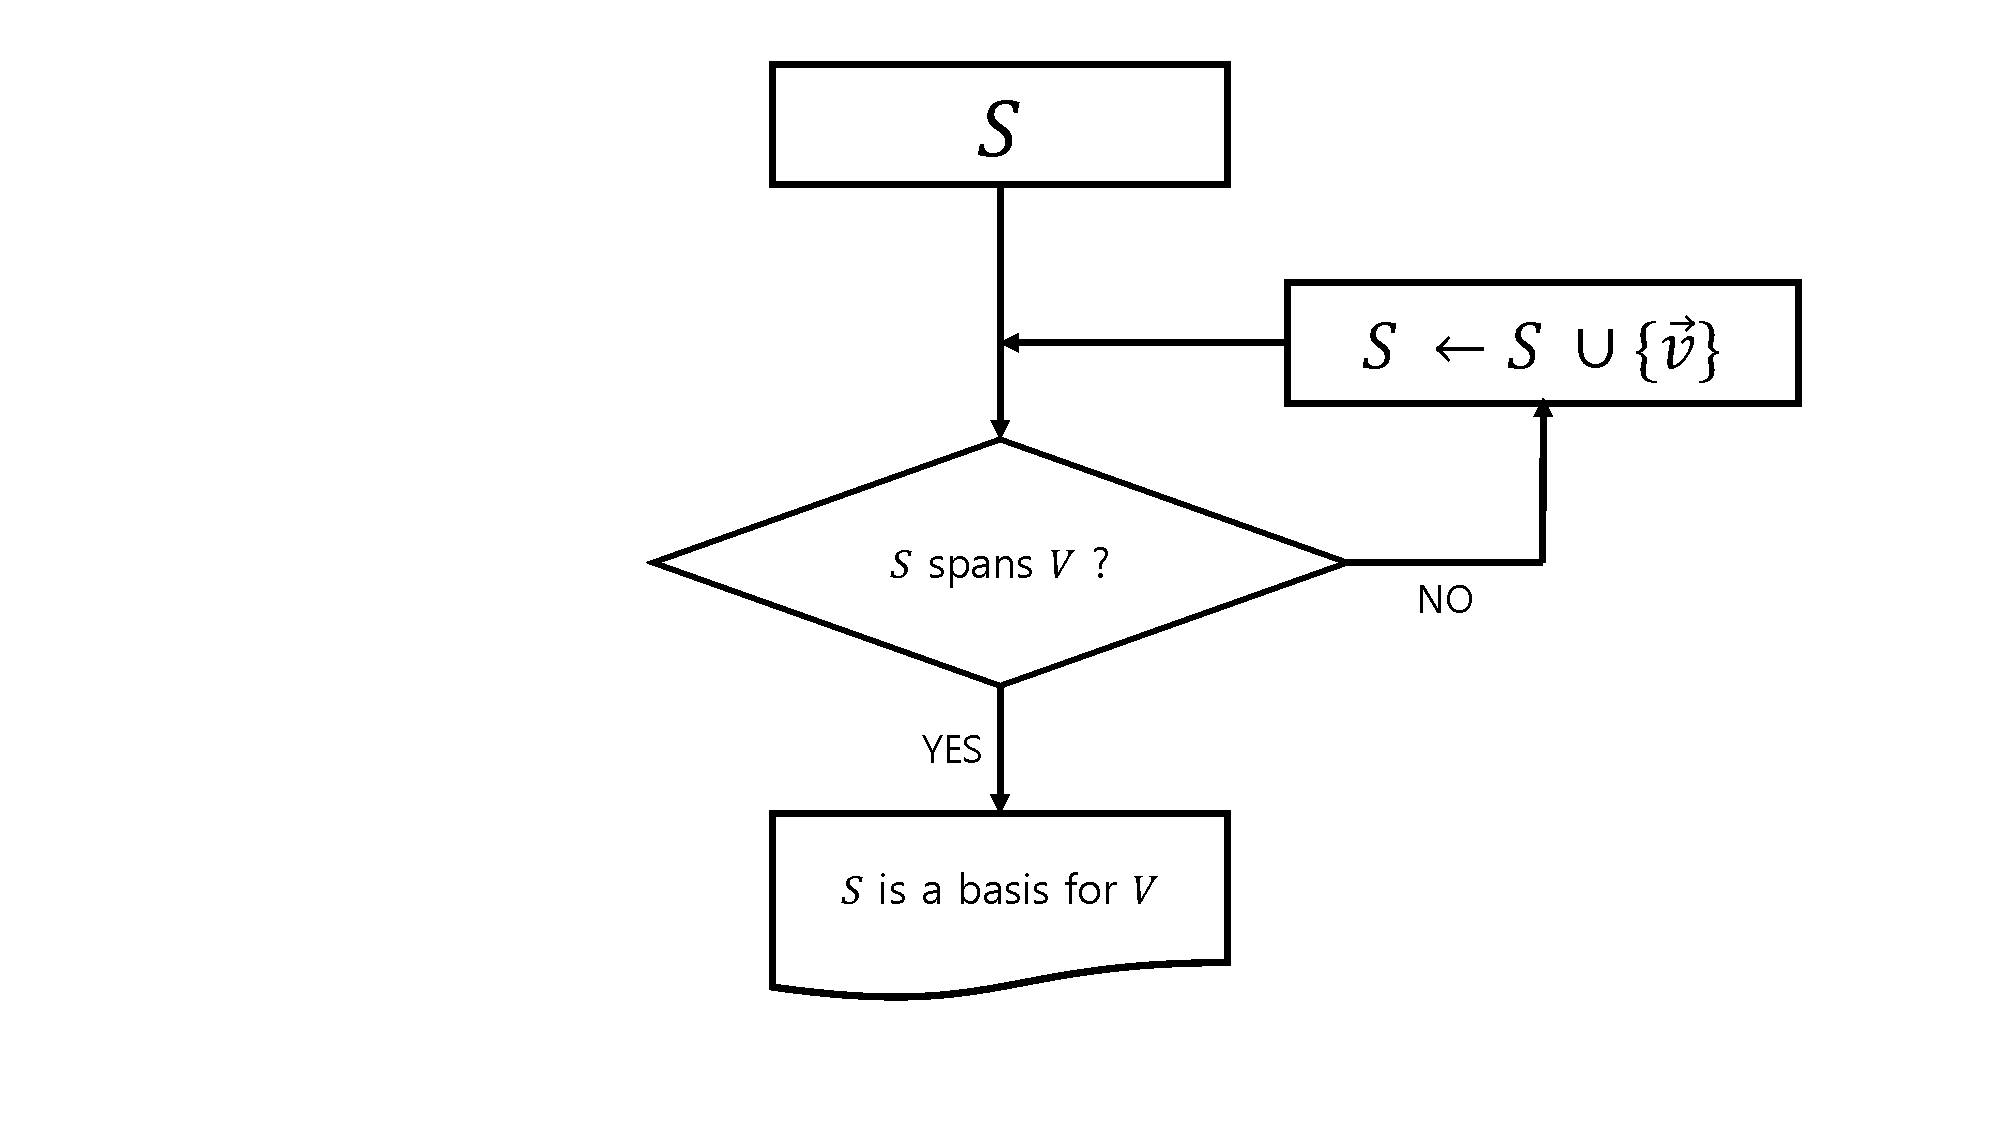
\includegraphics[scale = 0.3]{PlusTheorem.pdf}
			\end{center}
		\end{figure}
		This process terminates in finite operations since a linearly independent set in $V$ has at most $n$ vectors. The final $S$ forms a basis for $V$.
		\item \textbf{(Exercise 6.2 56)} Let $S$ be a spanning set for $V$. If $S$ is not linearly independent, there exist $\textbf{v} \in S$ which can be expressed as the linear combination of the other vectors. Redefine $S = S - \{\textbf{v}\}$, then $S$ is still a spanning set for $V$. (Exercise 6.2 55) Repeat the process until $S$ becomes a linearly independent set in $V$.
		\begin{figure}[H]
			\begin{center}
				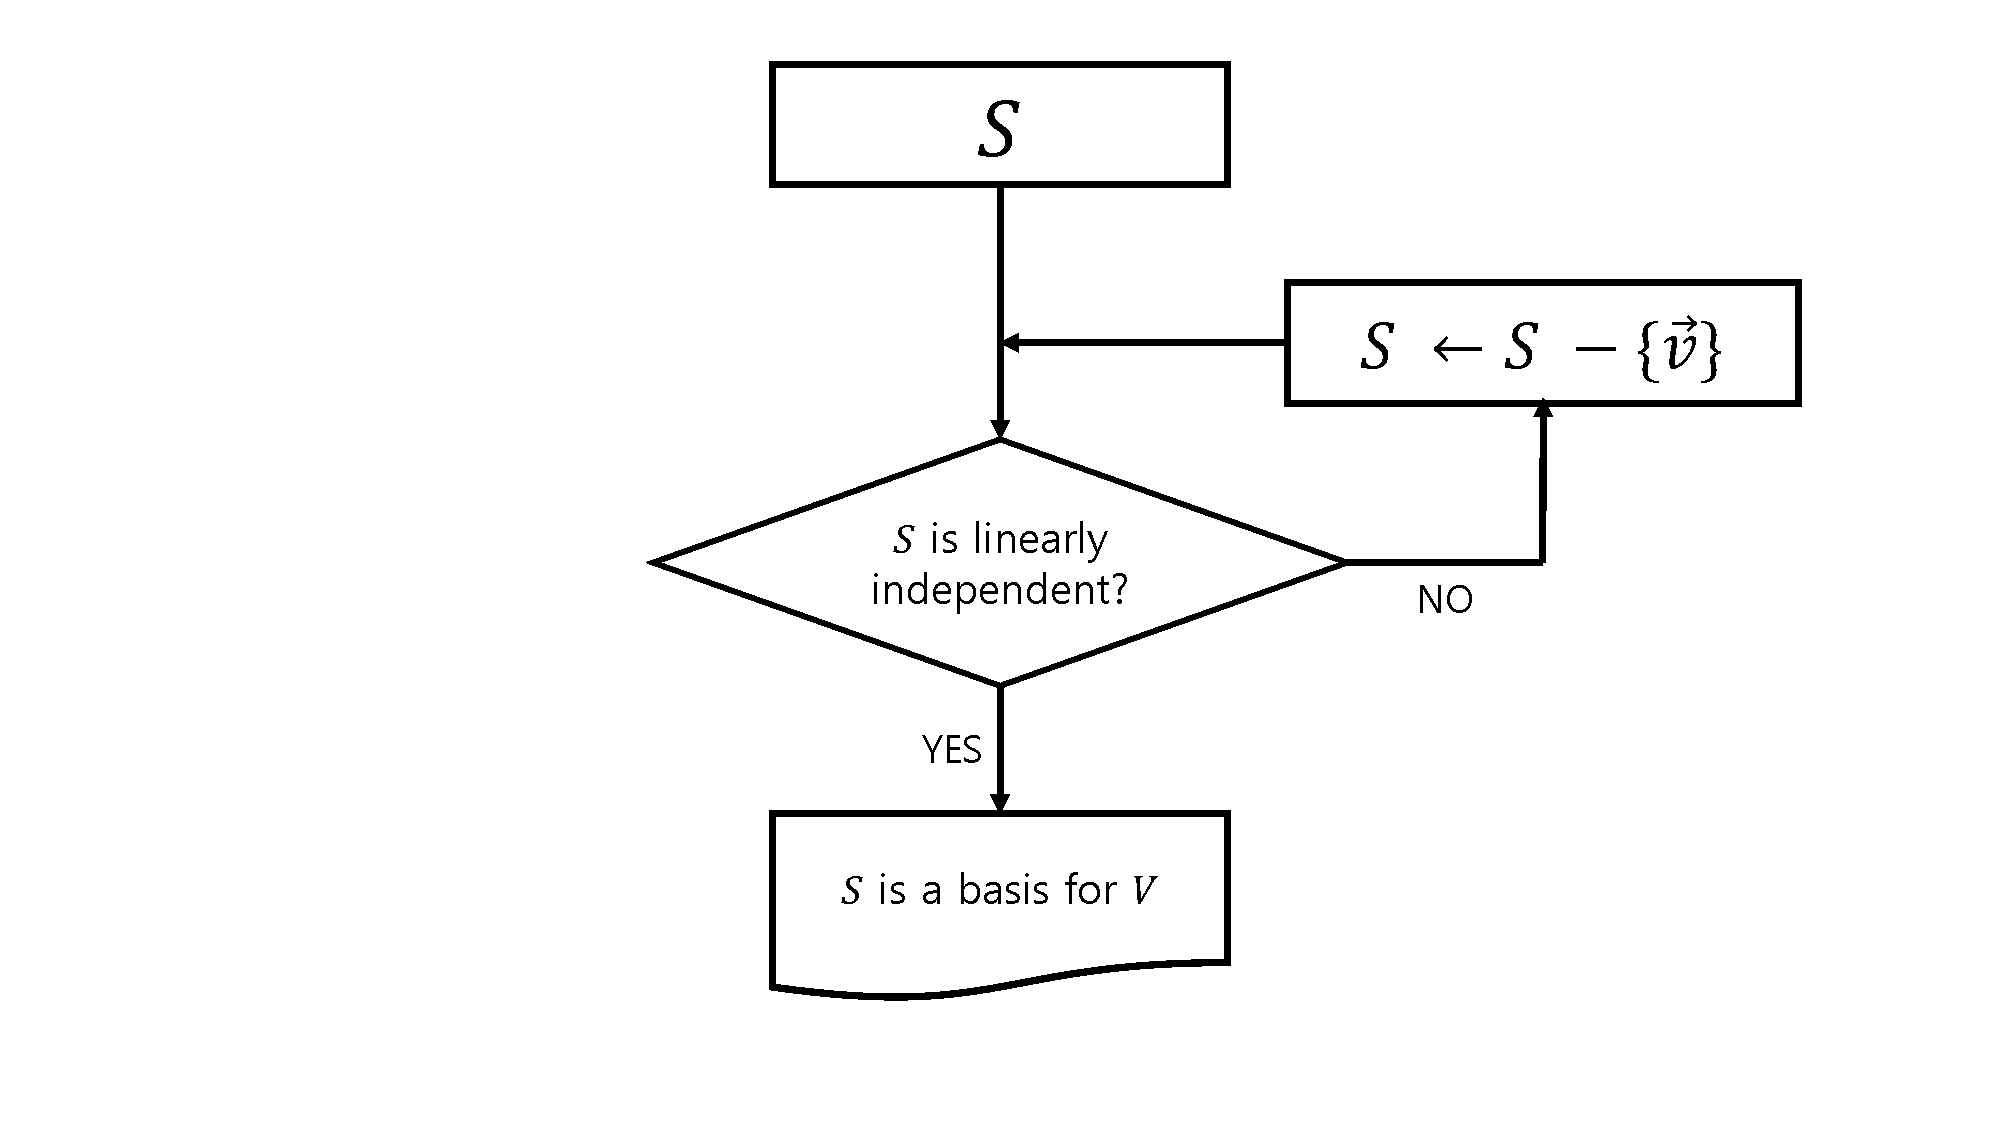
\includegraphics[scale = 0.3]{MinusTheorem.pdf}
			\end{center}
		\end{figure}
		This process terminates in finite operations since a spanning set for $V$ has at least $n$ vectors. The final $S$ forms a basis for $V$.
	\end{enumerate}
\end{proof}

\begin{theorem}
	Let $W$ be a subspace of a finite-dimensional vector space $V$.
	\begin{enumerate}
		\item $W$ is a finite-dimensional and $\dim W \le \dim V$.
		\item $\dim W = \dim V$ if and only if $W = V$.
	\end{enumerate}
\end{theorem}

\begin{proof}
	If $W$ is infinite-dimensional, it contains a infinite set which is linearly independent. However, by Theorem 6.10(a), a linearly independent set in $V$ has at most $n$ vectors. Thus $W$ is finite-dimensional, so let $\mathcal{B}$ be a basis for $W$.
	\begin{enumerate}
		\item (i) If $W = \{ \textbf{0} \}$, then $\dim W = 0 \le \dim V$. \\
		
		(ii) Suppose that $W$ is a nonzero subspace. Since $\mathcal{B}$ is a linearly independent set in $V$, by Theorem 6.10(e), $\mathcal{B}$ can be extended to a basis for $V$, which has $n$ vectors. Therefore, a basis for $W$ has lesser or equal than $n$ vectors, hence $\dim W \le n = \dim V$.
		\item ($\Rightarrow$) If $\dim W = \dim V = n$, then any basis $\mathcal{B}$ consists of $n$ vectors. Since $\mathcal{B}$ is a linearly independent set of $n$ vectors in $V$, it also forms a basis for $V$ by Theorem 6.10(c). Therefore, $V = W$.  \\
		
		($\Leftarrow$) If $W = V$, clearly $\dim W = \dim V$.
	\end{enumerate}
\end{proof}

\newpage
\section{Change of Basis}

6.3, 6.4, 6.5, 6.6 보기 전에 그림을 한 번 보고 가자.

\begin{figure}[H]
	\begin{center}
		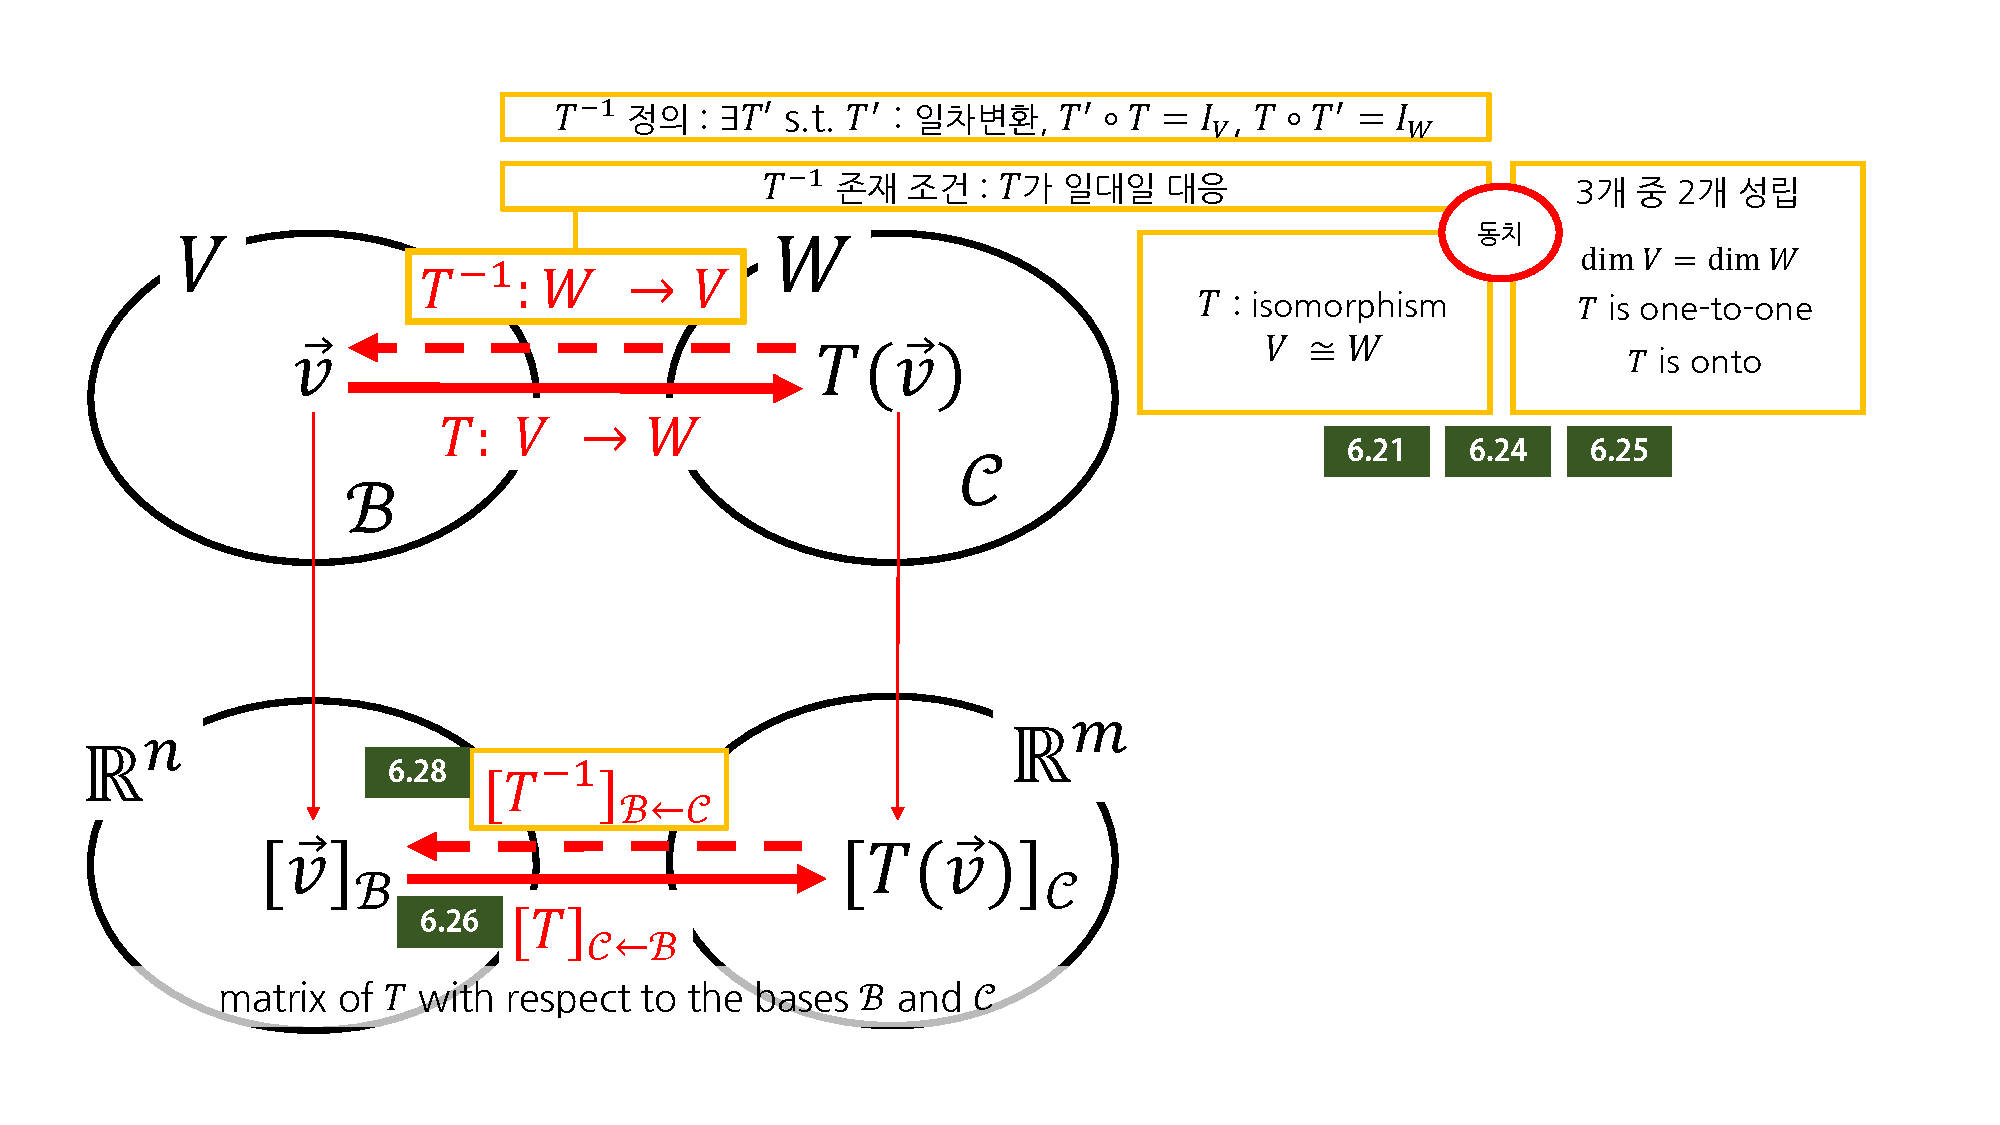
\includegraphics[scale = 0.5]{Figure1.pdf}
	\end{center}
\end{figure}

\begin{figure}[H]
	\begin{center}
		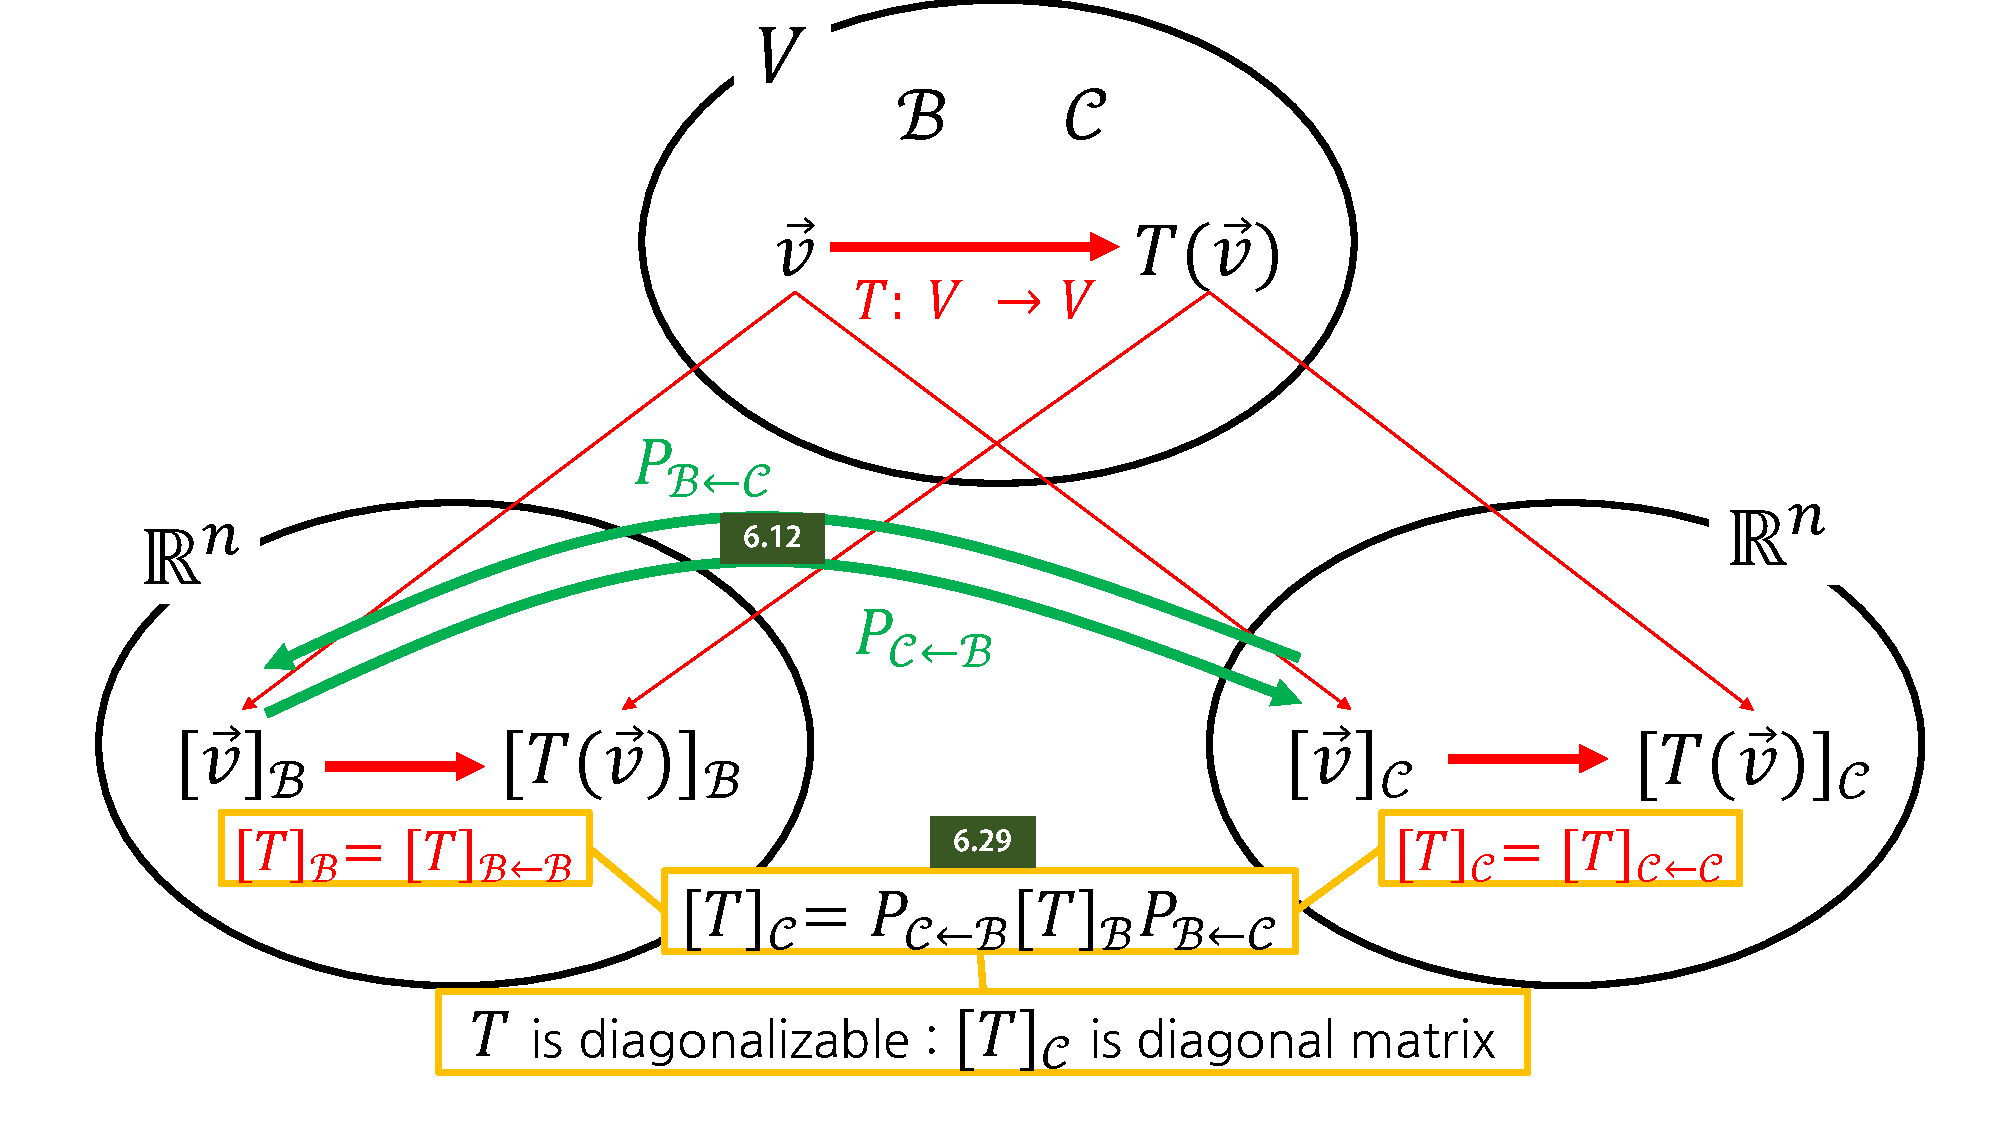
\includegraphics[scale = 0.4]{Figure2.pdf}
	\end{center}
\end{figure}

\newpage
\textit{Definition.} Let $\mathcal{B} = \{ \textbf{u}_1, \cdots, \textbf{u}_n \}$ and $\mathcal{C} = \{ \textbf{v}_1, \cdots, \textbf{v}_n \}$ be bases for a vector space $V$. The $n \times n$ matrix whose columns are the coordinate vectors $[\textbf{u}_1]_\mathcal{C}, \cdots, [\textbf{u}_n]_\mathcal{C}$ is denoted by $P_{\mathcal{C} \leftarrow \mathcal{B}}$ and is called the \textbf{change-of-basis matrix} from $\mathcal{B}$ to $\mathcal{C}$. \begin{equation*}
	P_{\mathcal{C} \leftarrow \mathcal{B}} = \begin{bmatrix}
		\left [ \textbf{u}_1 \right ]_\mathcal{C} & \cdots & \left [ \textbf{u}_n \right ]_\mathcal{C}
	\end{bmatrix}
\end{equation*}

\begin{theorem}
	Let $\mathcal{B} = \{ \textbf{u}_1, \cdots, \textbf{u}_n \}$ and $\mathcal{C} = \{ \textbf{v}_1, \cdots, \textbf{v}_n \}$ be bases for a vector space $V$.
	\begin{enumerate}
		\item $P_{\mathcal{C} \leftarrow \mathcal{B}}[\textbf{x}]_\mathcal{B} = [\textbf{x}]_\mathcal{C}$ for all $\textbf{x} \in V$.
		\item $P_{ \mathcal{C} \leftarrow \mathcal{B} }$ is the unique matrix $P$ with the property that $P[\textbf{x}]_\mathcal{B} = [\textbf{x}]_\mathcal{C}$ for all $\textbf{x} \in V$.
		\item $P_{ \mathcal{C} \leftarrow \mathcal{B} }$ is invertible and $\inv{(P_{ \mathcal{C} \leftarrow \mathcal{B} })} = P_{ \mathcal{B} \leftarrow \mathcal{C} }$.
	\end{enumerate}
\end{theorem}

\begin{proof}
	Let $\mathcal{B} = \{ \textbf{u}_1, \cdots, \textbf{u}_n \}$ and $\mathcal{C} = \{ \textbf{v}_1, \cdots, \textbf{v}_n \}$ be bases for a vector space $V$.
	\begin{enumerate}
		\item Let $\textbf{x}$ be a vector in $V$. Then there exist scalars $c_1, \cdots, c_n$ such that \begin{equation*}
		\textbf{x} = c_1\textbf{u}_1 + \cdots + c_n\textbf{u}_n
		\end{equation*} which implies that \begin{equation*}
		[\textbf{x}]_\mathcal{B} = \begin{bmatrix}
		c_1 \\ \vdots \\ c_n
		\end{bmatrix}
		\end{equation*} Then \begin{align*}
		[\textbf{x}]_\mathcal{C} &= [c_1\textbf{u}_1 + \cdots + c_n\textbf{u}_n]_\mathcal{C} \\
		&= c_1[\textbf{u}_1]_\mathcal{C} + \cdots + c_n[\textbf{u}_n]_\mathcal{C} \\
		&= \begin{bmatrix}
		\left[\textbf{u}_1\right]_\mathcal{C} & \cdots & [\textbf{u}_n]_\mathcal{C}
		\end{bmatrix} \begin{bmatrix}
		c_1 \\ \vdots \\ c_n
		\end{bmatrix} = P_{ \mathcal{C} \leftarrow \mathcal{B} }[\textbf{x}]_\mathcal{B}
		\end{align*}
		\item Suppose that $P = \begin{bmatrix}
			\textbf{p}_1 & \cdots & \textbf{p}_n
		\end{bmatrix}$ is an $n \times n$ matrix such that $P[\textbf{x}]_\mathcal{B} = [\textbf{x}]_\mathcal{C}$ for all $\textbf{x} \in V$. Since $[\textbf{u}_i]_\mathcal{B} = \textbf{e}_i$, for $i = 1, 2, \cdots, n$, \begin{equation*}
			\textbf{p}_i = P\textbf{e}_i = P[\textbf{u}_i]_\mathcal{B} = [\textbf{u}_i]_\mathcal{C}
		\end{equation*} Therefore, \begin{equation*}
			P = \begin{bmatrix}
				\textbf{p}_1 & \cdots & \textbf{p}_n
			\end{bmatrix} = \begin{bmatrix}
				\left[\textbf{u}_1\right]_\mathcal{C} & \cdots & [\textbf{u}_n]_\mathcal{C}
			\end{bmatrix} = P_{ \mathcal{C} \leftarrow \mathcal{B} }
		\end{equation*}
		\item Since $\mathcal{B}$ is a linearly independent set in $V$, the columns of $P_{ \mathcal{C} \leftarrow \mathcal{B} }$ are also linearly independent in $\mathbb{R}^n$ by Theorem 6.7, so $P_{ \mathcal{C} \leftarrow \mathcal{B} }$ is invertible by F.T.I.M. Since $P_{ \mathcal{C} \leftarrow \mathcal{B} }$ is invertible, for every $\textbf{x}$ in $V$, $[\textbf{x}]_\mathcal{B} = \inv{(P_{ \mathcal{C} \leftarrow \mathcal{B} })}[\textbf{x}]_\mathcal{C}$. Therefore, by Theorem 6.12(b), $\inv{(P_{ \mathcal{C} \leftarrow \mathcal{B} })} = P_{ \mathcal{B} \leftarrow \mathcal{C} }$. 
	\end{enumerate}
\end{proof}

\begin{theorem}
	Let $\mathcal{B} = \{ \textbf{u}_1, \cdots, \textbf{u}_n \}$ and $\mathcal{C} = \{ \textbf{v}_1, \cdots, \textbf{v}_n \}$ are basis for a vector space $V$. Let $B = \begin{bmatrix}
		\left[ \textbf{u}_1 \right]_\mathcal{E} & \cdots & \left[ \textbf{u}_n \right]_\mathcal{E}
	\end{bmatrix}$ and $C = \begin{bmatrix}
	\left[ \textbf{v}_1 \right]_\mathcal{E} & \cdots & \left[ \textbf{v}_n \right]_\mathcal{E}
	\end{bmatrix}$, where $\mathcal{E}$ is any basis for $V$. Then the row reduction applied to $n \times 2n$ augmented matrix $\begin{bmatrix} [c|c]
		C & B
	\end{bmatrix}$ produces \begin{equation*}
		\begin{bmatrix} [c|c]
		C & B
		\end{bmatrix} \rightarrow \begin{bmatrix} [c|c]
		I & P_{\mathcal{C} \leftarrow \mathcal{B}}
		\end{bmatrix}
	\end{equation*}
\end{theorem}

\begin{proof}
	Let scalars $p_{ij}$ such that \begin{equation*}
		[\textbf{u}_i]_\mathcal{C} = \begin{bmatrix}
			p_{1i} \\ \vdots \\ p_{ni}
		\end{bmatrix} \mbox{ for } i = 1, 2, \cdots, n
	\end{equation*} Then \begin{equation*}
		P_{ \mathcal{C} \leftarrow \mathcal{B} } = \begin{bmatrix}
			\left [\textbf{u}_1\right ]_\mathcal{C} & \cdots & [\textbf{u}_n]_\mathcal{C}
		\end{bmatrix} = \begin{bmatrix}
			p_{11} & \cdots & p_{1n} \\
			\vdots & & \vdots \\
			p_{n1} & \cdots & p_{nn}
		\end{bmatrix}
	\end{equation*}
	Let $\mathcal{E}$ be a basis for $V$. Since $\textbf{u}_i = p_{1i}\textbf{v}_1 + \cdots + p_{ni}\textbf{v}_n$, for $i = 1, 2, \cdots, n$, \begin{align*}
		[\textbf{u}_i]_\mathcal{E} &= [p_{1i}\textbf{v}_1 + \cdots + p_{ni}\textbf{v}_n]_\mathcal{E} = p_{1i}[\textbf{v}_1]_\mathcal{E} + \cdots + p_{ni}[\textbf{v}_n]_\mathcal{E} \\
		&= \begin{bmatrix}
			\left[\textbf{v}_1\right]_\mathcal{E} & \cdots & \left[\textbf{v}_n\right]_\mathcal{E}
		\end{bmatrix}\begin{bmatrix}
			p_{1i} \\ \vdots \\ p_{ni}
		\end{bmatrix}
	\end{align*}
	Thus, $\begin{bmatrix}
		p_{1i} \\ \vdots \\ p_{ni}
	\end{bmatrix}$ is the solution of the linear system with the augmented matrix given as \begin{equation*}
		\begin{bmatrix}[ccc|c]
			\left[\textbf{v}_1\right]_\mathcal{E} & \cdots & \left[\textbf{v}_n\right]_\mathcal{E} & \left[\textbf{u}_i\right]_\mathcal{E}
		\end{bmatrix}
	\end{equation*}
	Since the coefficient matrix is equal for each $i = 1, 2, \cdots, n$, $P$ can be obtained by row reducing the $n \times 2n$ augmented matrix \begin{equation*}
		\begin{bmatrix}[ccc|ccc]
			\left[\textbf{v}_1\right]_\mathcal{E} & \cdots & \left[\textbf{v}_n\right]_\mathcal{E} & \left[\textbf{u}_1\right]_\mathcal{E} & \cdots & \left[\textbf{u}_n\right]_\mathcal{E}
		\end{bmatrix} = \begin{bmatrix}[c|c]
		C & B
		\end{bmatrix}
	\end{equation*}
	Since $\textbf{v}_1, \cdots, \textbf{v}_n$ are linearly independent, $\left[\textbf{v}_1\right]_\mathcal{E}, \cdots , \left[\textbf{v}_n\right]_\mathcal{E}$ are also linearly independent by Theorem 6.7. Thus, by F.T.I.M, RREF of $C$ is $I$. Therefore, row reducing the augmented matrix will result in \begin{equation*}
		\begin{bmatrix}[c|c]
		C & B
		\end{bmatrix} \rightarrow \begin{bmatrix}[c|c]
		I & P_{ \mathcal{C} \leftarrow \mathcal{B} }
		\end{bmatrix}
	\end{equation*}
\end{proof}

% 3.6 추가할 것. %
\section{Linear Transformations + 3.6 Part I}

\textit{Definition.} A \textbf{linear transformation} from a vector space $V$ to a vector space $W$ is a mapping $T: V \rightarrow W$ such that for all $\textbf{u}$ and $\textbf{v}$ in $V$ and for all scalars $c$, \begin{enumerate}
	\item $T(\textbf{u} + \textbf{v}) = T(\textbf{u}) + T(\textbf{v})$
	\item $T(c\textbf{u}) = cT(\textbf{u})$
\end{enumerate}

\begin{theorem}
	Let $T: V \rightarrow W$ be a linear transformation. \begin{enumerate}
		\item $T(\textbf{0}) = \textbf{0}$
		\item $T(-\textbf{v}) = -T(\textbf{v})$ for all $\textbf{v} \in V$
		\item $T(\textbf{u} - \textbf{v}) = T(\textbf{u}) - T(\textbf{v})$ for all $\textbf{u}, \textbf{v} \in V$
	\end{enumerate}
\end{theorem}

\begin{proof}
	Let $T: V \rightarrow W$ be a linear transformation.
	\begin{enumerate}
		\item Let $\textbf{v}$ be a vector in $V$. Then \begin{align*}
			T(\textbf{0}) = T(0\textbf{v}) = 0T(\textbf{v}) = \textbf{0}
		\end{align*}
		\item \textbf{(Exercise 6.4 21)} For any $\textbf{v} \in V$, \begin{equation*}
			T(-\textbf{v}) = T((-1)\textbf{v}) = (-1)T(\textbf{v}) = -T(\textbf{v})
		\end{equation*}
		\item For any $\textbf{u}, \textbf{v} \in V$, \begin{equation*}
			T(\textbf{u} - \textbf{v}) = T(\textbf{u} + (-1)\textbf{v}) = T(\textbf{u}) + (-1)T(\textbf{v}) = T(\textbf{u}) - T(\textbf{v})
		\end{equation*}
	\end{enumerate}
\end{proof}

\textit{Note.} Theorem 6.14(a)에서 $V$의 zero vector와 $W$의 zero vector를 잘 구분하자.

\begin{theorem}
	Let $T: V \rightarrow W$ be a linear transformation and let $\mathcal{B} = \{ \textbf{v}_1, \cdots, \textbf{v}_n \}$ is a spanning set for $V$. Then $T(\mathcal{B}) = \{ T(\textbf{v}_1), \cdots, T(\textbf{v}_n) \}$ is the spanning set for range of $T$.
\end{theorem}

\begin{proof}
	Let $\textbf{w}$ be a vector in range($T$), then there exists a vector $\textbf{v} \in V$ such that $\textbf{w} = T(\textbf{v})$. Since $\mathcal{B}$ spans $V$, there exist scalars $c_1, \cdots, c_n$ such that \begin{equation*}
		\textbf{v} = c_1\textbf{v}_1 + \cdots + c_n\textbf{v}_n
	\end{equation*} Thus, \begin{equation*}
		\textbf{w} = T(\textbf{v}) = T(c_1\textbf{v}_1 + \cdots + c_n\textbf{v}_n) = c_1T(\textbf{v}_1) + \cdots + c_nT(\textbf{v}_n)
	\end{equation*} Therefore, $\textbf{w}$ is in span($T(\mathcal{B})$), hence $T(\mathcal{B})$ is a spanning set for range($T$).
\end{proof}

\textit{Note.} Spanning set은 이렇게 되는데, linear independence는 $T$가 one-to-one이어야 성립한다. (Theorem 6.22) \\

\textit{Definition.} If $T: U \rightarrow V$ and $S: V \rightarrow W$ are linear transformations, then the \textbf{composition of S with T} is the mapping $S \circ T$, defined by \begin{equation*}
	(S \circ T)(\textbf{u}) = S(T(\textbf{u}))
\end{equation*}

\begin{theorem}
	If $T: U \rightarrow V$ and $S: V \rightarrow W$ are linear transformations, then $S \circ T: U \rightarrow W$ is a linear transformation.
\end{theorem}

\textbf{Theorem 3.32 : Part 1} \\
 Let $T: \mathbb{R}^m \rightarrow \mathbb{R}^n$ and $S: \mathbb{R}^n \rightarrow \mathbb{R}^p$ be linear transformations. Then $S \circ T: \mathbb{R}^m \rightarrow \mathbb{R}^p$ is a linear transformation. \\

\begin{proof}
	Let $\textbf{u}, \textbf{v}$ be vectors in $U$, and let $c$ be a scalar. Then \begin{align*}
		(S \circ T)(\textbf{u} + \textbf{v}) &= S(T(\textbf{u} + \textbf{v})) \\
		&= S(T(\textbf{u}) + T(\textbf{v}) \\
		&= S(T(\textbf{u})) + S(T(\textbf{v})) = (S \circ T)(\textbf{u}) + (S \circ T)(\textbf{v})
	\end{align*}
	Also, \begin{align*}
		(S \circ T)(c\textbf{u}) &= S(T(c\textbf{u})) \\
		&= S(cT(\textbf{u})) \\
		&= cS(T(\textbf{u})) = c(S \circ T)(\textbf{u})
	\end{align*}
	Therefore, $S \cdot T$ is a linear transformation.
\end{proof}

\textit{Definition.} A linear transformation $T: V \rightarrow W$ is \textbf{invertible} if there exists a linear transformation $T': W \rightarrow V$ such that \begin{equation*}
	T' \circ T = I_V \mbox{ and } T \circ T' = I_W
\end{equation*} and such linear transformation $T'$ is called an \textbf{inverse} for $T$.

\begin{theorem}
	If $T$ is an invertible linear transformation, then its inverse is unique.
\end{theorem}

\begin{proof}
	\textbf{(Exercise 6.4 31)} Let $T: V \rightarrow W$ be an invertible linear transformation. Suppose that $T': W \rightarrow V$ and $T'': W \rightarrow V$ are both inverses of $T$, then \begin{align*}
		T \circ T' = T \circ T'' = I_W \mbox{ and } T' \circ T = T'' \circ T = I_V
	\end{align*} Thus, \begin{align*}
		T' = I_V \circ T' = (T'' \circ T) \circ T' = T'' \circ (T \circ T') = T'' \circ I_W = T''
	\end{align*} Therefore, the inverse of $T$ is unique.
\end{proof}

\section{Kernel and Range}
\textit{Definition.} Let $T: V \rightarrow W$ be a linear transformation. The \textbf{kernel} of $T$, denoted by ker($T$), is defined by \begin{equation*}
	\textnormal{ker}(T) = \{ \textbf{v} \in V \vert T(\textbf{v}) = \textbf{0} \}
\end{equation*}
The \textbf{range} of $T$, denoted by range($T$), is defined by \begin{equation*}
	\textnormal{range}(T) = \{\textbf{w} \in W \vert \textbf{w} = T(\textbf{v}) \mbox{ for some } \textbf{v} \in V \}
\end{equation*}

\textit{Note.} ker($T$)는 $V$의 vector들의 집합이고, range($T$)는 $W$의 vector들의 집합임을 상기하자.

\begin{theorem}
	Let $T: V \rightarrow W$ be a linear transformation. \begin{enumerate}
		\item ker($T$) is a subspace of $V$.
		\item range($T$) is a subspace of $W$.
	\end{enumerate}
\end{theorem}

\begin{proof}
	Let $T: V \rightarrow W$ be a linear transformation.
	\begin{enumerate}
		\item Since $T(\textbf{0}) = \textbf{0}$ by Theorem 6.14(a), $\textbf{0} \in \ker(T)$ so ker($T$) is a nonempty set. Let $\textbf{u}, \textbf{v}$ be vectors in ker($T$), and let $c$ be a scalar, then \begin{align*}
			&T(\textbf{u} + \textbf{v}) = T(\textbf{u}) + T(\textbf{v}) = \textbf{0} + \textbf{0} = \textbf{0} \\
			&T(c\textbf{u}) = cT(\textbf{u}) = c\textbf{0} = \textbf{0}
		\end{align*} Therefore $\textbf{u} + \textbf{v} \in \ker(T)$ and $c\textbf{u} \in \ker(T)$, hence ker($T$) is a subspace of $V$ by Theorem 6.2.
		\item Since $T(\textbf{0}) = \textbf{0}$ by Theorem 6.14(a), $\textbf{0} \in$ range($T$) so range($T$) is a nonempty set. Let $\textbf{w}_1, \textbf{w}_2$ be vectors in range($T$) and let $c$ be a scalar. Then there exist $\textbf{v}_1, \textbf{v}_2 \in V$ such that $T(\textbf{v}_1) = \textbf{w}_1$ and $ T(\textbf{v}_2) = \textbf{w}_2$. Then \begin{align*}
			&\textbf{w}_1 + \textbf{w}_2 = T(\textbf{v}_1) + T(\textbf{v}_2) = T(\textbf{v}_1 + \textbf{v}_2) \\
			&c\textbf{w}_1 = cT(\textbf{v}_1) = T(c\textbf{v}_1)
		\end{align*} Therefore $\textbf{w}_1 + \textbf{w}_2 \in$ range($T$) and $c\textbf{w}_1 \in $ range($T$), hence range($T$) is a subspace of $V$ by Theorem 6.2.
	\end{enumerate}
\end{proof}

이제 ker($T$)와 range($T$)가 vector space임을 증명했으니 그 dimension으로 rank와 nullity를 정의할 수 있다. \\

\textit{Definition.} Let $T: V \rightarrow W$ be a linear transformation. Then the rank and nullity of $T$, denoted by rank($T$) and nullity($T$), is defined by \begin{equation*}
	\textnormal{rank}(T) = \dim(\textnormal{range}(T)) \mbox{ and } \textnormal{nullity}(T) = \dim(\ker{(T)})
\end{equation*}

\begin{theorem}[The Rank Theorem : for Linear Transformation]
	Let $T: V \rightarrow W$ be a linear transformation from a finite-dimensional vector space $V$ to a vector space $W$. Then \begin{equation*}
		\textnormal{rank}(T) + \textnormal{nullity}(T) = \dim V
	\end{equation*}
\end{theorem}

\begin{proof}
	Let $n = \dim V$, and let $\{ \textbf{v}_1, \cdots, \textbf{v}_k \}$ be a basis for ker($T$). By Theorem 6.10(e), $\{ \textbf{v}_1, \cdots, \textbf{v}_k \}$ can be extended to a basis $\mathcal{B} = \{ \textbf{v}_1, \cdots, \textbf{v}_k, \textbf{v}_{k+1}, \cdots, \textbf{v}_n \}$ for $V$. \\
	
	Let $\mathcal{C} = \{ T(\textbf{v}_{k+1}), \cdots, T(\textbf{v}_n) \}$, then $\mathcal{C}$ is a subset of range($T$). Let $\textbf{w}$ be a vector in range($T$), then there exists $\textbf{v} \in V$ such that $T(\textbf{v}) = \textbf{w}$. Then there exist scalars $c_1, \cdots, c_n$ such that \begin{equation*}
		\textbf{v} = c_1\textbf{v}_1 + \cdots + c_k\textbf{v}_k + c_{k+1}\textbf{v}_{k+1} + \cdots + c_n\textbf{v}_n
	\end{equation*} Then \begin{align*}
		\textbf{w} = T(\textbf{v}) &= T(c_1\textbf{v}_1 + \cdots + c_k\textbf{v}_k + c_{k+1}\textbf{v}_{k+1} + \cdots + c_n\textbf{v}_n) \\
		&= c_1T(\textbf{v}_1) + \cdots + c_kT(\textbf{v}_k) + c_{k+1}T(\textbf{v}_{k+1}) + \cdots + c_nT(\textbf{v}_n) \\
		&= c_{k+1}T(\textbf{v}_{k+1}) + \cdots + c_nT(\textbf{v}_n)
	\end{align*} Thus $\textbf{w} \in $ span($\mathcal{C}$), which implies that $\mathcal{C}$ is a spanning set for range($T$). \\
	
	Now, consider the equation \begin{equation*}
		c_{k+1}T(\textbf{v}_{k+1}) + \cdots + c_nT(\textbf{v}_n) = \textbf{0}
	\end{equation*} Then $T(c_{k+1}\textbf{v}_{k+1} + \cdots + c_n\textbf{v}_n) = \textbf{0}$, so $c_{k+1}\textbf{v}_{k+1} + \cdots + c_n\textbf{v}_n \in \ker(T)$. Since $\mathcal{B}$ is a basis for $\ker(T)$, there exist scalars $c_1, \cdots, c_k$ such that \begin{equation*}
		c_{k+1}\textbf{v}_{k+1} + \cdots + c_n\textbf{v}_n = c_1\textbf{v}_1 + \cdots + c_k\textbf{v}_k
	\end{equation*} Since $\textbf{v}_1, \cdots, \textbf{v}_n$ are linearly independent, this implies that $c_1 = \cdots = c_k = c_{k+1} = \cdots = c_n = 0$. Therefore, $T(\textbf{v}_{k+1}), \cdots, T(\textbf{v}_n)$ are linearly independent. \\
	
	Since $\mathcal{C}$ is linearly independent and is a spanning set for range($T$), it forms a basis for range($T$). Therefore, \begin{equation*}
		\textnormal{rank}(T) + \textnormal{nullity}(T) = (n - k) + k = n = \dim V
	\end{equation*}
\end{proof}

\textit{Definition.} A linear transformation $T: V \rightarrow W$ is called \textbf{one-to-one} if $T$ maps distinct vectors in $V$ to distinct vectors in $W$. That is, for vectors $\textbf{v}, \textbf{w}$ in $V$, \begin{equation*}
	\textbf{v} \neq \textbf{w} \Rightarrow T(\textbf{v}) \neq T(\textbf{w})
\end{equation*}

\textit{Definition.} A linear transformation $T: V \rightarrow W$ is called \textbf{onto} if range($T$) = $W$. That is, \begin{equation*}
	^\forall \textbf{w} \in W, ^\exists \textbf{v} \in V \mbox{ such that } T(\textbf{v}) = \textbf{w}
\end{equation*}

\begin{theorem}
	A linear transformation $T: V \rightarrow W$ is one-to-one if and only if ker($T$) = $\{ \textbf{0} \}$.
\end{theorem}

\begin{proof}
	($\Rightarrow$) Suppose that there exists a nonzero vector $\textbf{v}$ in ker($T$). Then $T(\textbf{v}) = T(\textbf{0}) = \textbf{0}$, which is a contradiction since $T$ is one-to-one. Therefore, ker($T$) = $\{ \textbf{0} \}$. \\
	
	($\Leftarrow$) Let $\textbf{u}, \textbf{v} \in V$ such that $T(\textbf{u}) = T(\textbf{v})$. Since ker($T$) = $\{\textbf{0}\}$ and $T(\textbf{u} - \textbf{v}) = T(\textbf{u}) - T(\textbf{v}) = \textbf{0}$, $\textbf{u} - \textbf{v} = \textbf{0}$. Therefore, $\textbf{u} = \textbf{v}$ and hence, $T$ is one-to-one.
\end{proof}

\begin{theorem}
	Let $\dim V = \dim W = n$. Then a linear transformation $T: V \rightarrow W$ is one-to-one if and only if it is onto.
\end{theorem}

\begin{proof}
	($\Rightarrow$) If $T$ is one-to-one, ker($T$) = $\{ \textbf{0} \}$ by Theorem 6.20, so nullity($T$) = 0. By the Rank Theorem, rank($T$) = dim(range($T$)) = 0. Since range($T$) is a subspace of $W$, range($T$) = $W$ by Theorem 6.11(b). Therefore, $T$ is onto. \\
	
	($\Leftarrow$) If $T$ is onto, then rank($T$) = dim(range($T$)) = dim($W$) = $n$. By the Rank Theorem, nullity($T$) = dim(ker($T$)) = 0, so ker($T$) = $\{\textbf{0}\}$. Therefore, by Theorem 6.20, $T$ is one-to-one.
\end{proof}

\begin{theorem}
	Let $T: V \rightarrow W$ be a one-to-one linear transformation. If $S = \{ \textbf{v}_1, \cdots, \textbf{v}_k \}$ is a linearly independent set in $V$, Then $T(S) = \{ T(\textbf{v}_1), \cdots, T(\textbf{v}_k) \}$ is a linearly independent set in $W$.
\end{theorem}
\begin{proof}
	Consider the equation \begin{equation*}
		c_1T(\textbf{v}_1) + \cdots + c_kT(\textbf{v}_k) = \textbf{0}
	\end{equation*} Then $T(c_1\textbf{v}_1 + \cdots + c_k\textbf{v}_k) = \textbf{0}$, so $c_1\textbf{v}_1 + \cdots + c_k\textbf{v}_k \in \ker(T)$. Since $T$ is one-to-one, ker($T$) = $\{\textbf{0}\}$ by Theorem 6.20, so $c_1\textbf{v}_1 + \cdots + c_k\textbf{v}_k = \textbf{0}$. This implies that $c_1 = \cdots = c_k = 0$, since $\textbf{v}_1, \cdots, \textbf{v}_k$ are linearly independent. Therefore, $T(\textbf{v}_1), \cdots, T(\textbf{v}_k)$ are also linearly independent.
\end{proof}

\begin{corollary}
	Let $\dim V = \dim W = n$. Then a one-to-one linear transformation $T: V \rightarrow W$ maps a basis for $V$ to a basis for $W$.
\end{corollary}

\begin{proof}
	If $\mathcal{B}$ is a basis of $V$, Theorem 6.15 and Theorem 6.22 together gives that $T(\mathcal{B})$ is a linearly independent set in $W$ and is a spanning set for $W$. Therefore, $T(\mathcal{B})$ is a basis for $W$.
\end{proof}

\begin{theorem}
	A linear transformation $T: V \rightarrow W$ is invertible if and only if it is one-to-one and onto.
\end{theorem}

\begin{proof}
	($\Rightarrow$) Suppose that $T$ is invertible. Then there exists a linear transformation $\inv{T}: W \rightarrow V$ such that \begin{equation*}
		\inv{T} \circ T = I_V \mbox{ and } T \circ \inv{T} = I_W
	\end{equation*}
	(i) Let $\textbf{v}$ be a vector in ker($T$), then $T(\textbf{v}) = \textbf{0}$. Then, \begin{equation*}
		I_V(\textbf{v}) = (\inv{T} \circ T)(\textbf{v}) = \inv{T}(T(\textbf{v})) = \inv{T}(\textbf{0}) = \textbf{0}
	\end{equation*} Thus, $\textbf{v} = \textbf{0}$, which implies that ker($T$) = $\{\textbf{0}\}$. Therefore, $T$ is one-to-one by Theorem 6.20. \\
	
	(ii) Let $\textbf{w}$ be a vector in $W$, and let $\textbf{v} = \inv{T}(\textbf{w})$. Then \begin{equation*}
		T(\textbf{v}) = T(\inv{T}(\textbf{w})) = (T \circ \inv{T})(\textbf{w}) = I_W(\textbf{w}) = \textbf{w}
	\end{equation*} Therefore, $\textbf{w} \in $ range($T$). Therefore, range($T$) = $W$ and $T$ is onto. \\
	
	($\Leftarrow$) Suppose that $T: V \rightarrow W$ is one-to-one and onto. For every vector $\textbf{w}$ in $W$, there exists a unique vector $\textbf{v} \in V$ such that $T(\textbf{v}) = \textbf{w}$, since $T$ is one-to-one and onto. Let $T': W \rightarrow V$ be a transformation which maps $\textbf{w}$ into such $\textbf{v}$. \\
	
	Let $\textbf{w}_1, \textbf{w}_2$ be vectors in $W$ and $c$ a scalar. Let $\textbf{v}_1, \textbf{v}_2$ be vectors such that $T(\textbf{v}_1) = \textbf{w}_1$ and $T(\textbf{v}_2) = \textbf{w}_2$, then $T'(\textbf{w}_1) = \textbf{v}_1$ and $T'(\textbf{w}_2) = \textbf{v}_2$. Then \begin{align*}
		T(\textbf{v}_1 + \textbf{v}_2) = T(\textbf{v}_1) &+ T(\textbf{v}_2) = \textbf{w}_1 + \textbf{w}_2 \\
		T(c\textbf{v}_1) &= cT(\textbf{v}_1) = c\textbf{w}_1
	\end{align*}
	so $T'(\textbf{w}_1 + \textbf{w}_2) = \textbf{v}_1 + \textbf{v}_2 = T'(\textbf{w}_1) + T'(\textbf{w}_2)$ and $T'(c\textbf{w}_1) = c\textbf{v}_1 = cT(\textbf{w}_1)$. Therefore, $T'$ is a linear transformation. \\
	
	Also, for any vector $\textbf{v} \in V$, let $\textbf{w} = T(\textbf{v})$ then $T'(\textbf{w}) = \textbf{v}$, so \begin{align*}
		(T' \circ T)(\textbf{v}) &= T'(T(\textbf{v})) = T'(\textbf{w}) = \textbf{v} \\
		(T \circ T')(\textbf{w}) &= T(T'(\textbf{w})) = T(\textbf{v}) = \textbf{w}
	\end{align*} This implies that $T' \circ T = I_V$ and $T \circ T' = I_W$. \\
	
	Therefore, $T'$ is an inverse of $T$, hence $T$ is invertible.
\end{proof}

\textit{Definition.} A linear transformation $T: V \rightarrow W$ is called \textbf{isomorphism} if it is one-to-one and onto. If $V$ and $W$ are two vector spaces such that there exists an isomorphism from $V$ to $W$, then $V$ is called to be \textbf{isomorphic} to $W$ and denoted by $V \cong W$.

\begin{theorem}
	Let $V$ and $W$ be two finite-dimensional vector spaces, over the same field of scalars. Then $V \cong W$ if and only if $\dim V = \dim W$.
\end{theorem}

\begin{proof}
	Let $n = \dim V$. \\
	
	($\Rightarrow$) If $V \cong W$, then there exists a linear transformation $T: V \rightarrow W$ which is an isomorphism. Since $T$ is one-to-one, ker($T$) = $\{\textbf{0}\}$ so nullity($T$) = 0, and by Rank Theorem, rank($T$) = $n$. Since $T$ is onto, $W$ = range($T$) so $\dim W$ = dim(range($T$)) = rank($T$) = $n$. \\
	
	($\Leftarrow$) Let $n = \dim V = \dim W$. Let $\mathcal{B} = \{\textbf{v}_1, \cdots, \textbf{v}_n\}$ be a basis for $V$ and let $\mathcal{C} = \{\textbf{w}_1, \cdots, \textbf{w}_n\}$ be a basis for $W$. For every vector $\textbf{v}$ in $V$, there exist scalars $c_1, \cdots, c_n$ such that \begin{equation*}
		\textbf{v} = c_1\textbf{v}_1 + \cdots + c_n\textbf{v}_n
	\end{equation*} then let $T: V \rightarrow W$ be defined by \begin{equation*}
		T(\textbf{v}) = c_1\textbf{w}_1 + \cdots + c_n\textbf{w}_n
	\end{equation*}
	(i) First we prove that $T$ is a linear transformation. Let $\textbf{u}, \textbf{v} \in V$, then there exist scalars $c_1, \cdots, c_n$ and $d_1, \cdots, d_n$ such that $\textbf{u} = c_1\textbf{v}_1 + \cdots + c_n\textbf{v}_n$ and $\textbf{v} = d_1\textbf{v}_1 + \cdots + d_n\textbf{v}_n$. Since $\textbf{u} + \textbf{v} = (c_1 + d_1)\textbf{v}_1 + \cdots + (c_n + d_n)\textbf{v}_n$, \begin{align*}
		T(\textbf{u} + \textbf{v}) &= (c_1 + d_1)\textbf{w}_1 + \cdots + (c_n + d_n)\textbf{w}_n \\ &= (c_1\textbf{w}_1 + \cdots + c_n\textbf{w}_n) + (d_1\textbf{w}_1 + \cdots + c_n\textbf{w}_n) = T(\textbf{u}) + T(\textbf{v})
	\end{align*} And for any scalar $c$, $c\textbf{u} = cc_1\textbf{v}_1 + \cdots + cc_n\textbf{v}_n$, so \begin{align*}
		T(c\textbf{u}) &= cc_1\textbf{w}_1 + \cdots + cc_n\textbf{w}_n \\
		&= c(c_1\textbf{w}_1 + \cdots + c_n\textbf{w}_n) = cT(\textbf{u})
	\end{align*} Thus $T$ is a linear transformation. \\
	
	(ii) Suppose that $\textbf{v} \in \ker(T)$, then there exist scalars $c_1, \cdots, c_n$ such that $\textbf{v} = c_1\textbf{v}_1 + \cdots + c_n\textbf{v}_n$. Then \begin{equation*}
		T(\textbf{v}) = c_1\textbf{w}_1 + \cdots + c_n\textbf{w}_n = \textbf{0}
	\end{equation*} Since $\textbf{w}_1, \cdots, \textbf{w}_n$ are linearly independent, $c_1 = \cdots = c_n = 0$ so $\textbf{v} = \textbf{0}$. Therefore, ker($T$) = $\{\textbf{0}\}$, hence $T$ is one-to-one by Theorem 6.20. \\
	
	(iii) Since $\dim V = \dim W$ and $T$ is one-to-one, $T$ is onto by Theorem 6.21. \\
	
	By (i), (ii), and (iii), $T$ is an isomorphism, therefore $V$ and $W$ are isomorphic.
\end{proof}

\textit{Note.} 6.5 요약 : `항상 False'의 증명은 Exercise 6.5 35에 있음.
\begin{figure}[H]
	\begin{center}
		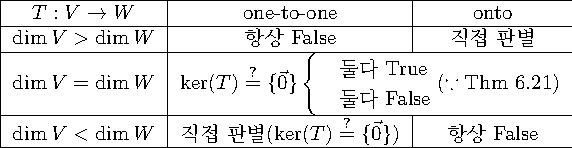
\includegraphics[scale = 1.0]{one-to-one+onto.pdf}
	\end{center}
\end{figure}

\section{The Matrix of a Linear Transformation + 3.6 Part II}

\textit{Definition.} Let $V$ and $W$ be vector spaces with $\dim V = n$ and $\dim W = m$. Let $\mathcal{B}$ and $\mathcal{C}$ be bases for $V$ and $W$, respectively, where $\mathcal{B} = \{ \textbf{v}_1, \cdots, \textbf{v}_n \}$. The \textbf{matrix of $T$ with respect to the bases $\mathcal{B}$ and $\mathcal{C}$}, denoted by $[T]_{ \mathcal{C} \leftarrow \mathcal{B} }$, is the $m \times n$ matrix defined by \begin{equation*}
	[T]_{ \mathcal{C} \leftarrow \mathcal{B} } = \begin{bmatrix}
	\left[ T(\textbf{v}_1) \right]_\mathcal{C} & \cdots & \left[ T(\textbf{v}_n) \right]_\mathcal{C}
	\end{bmatrix}
\end{equation*}
If $V = W$ and $\mathcal{B} = \mathcal{C}$, we write $[T]_{ \mathcal{B} \leftarrow \mathcal{B} }$ as $[T]_\mathcal{B}$ for short.

\begin{theorem}
	Let $V$ and $W$ be two finite-dimensional vector spaces with bases $\mathcal{B}$ and $\mathcal{C}$, respectively. If $T: V \rightarrow W$ is a linear transformation, \begin{equation*}
		[T]_{\mathcal{C} \leftarrow \mathcal{B}}[\textbf{v}]_\mathcal{B} = [T(\textbf{v})]_\mathcal{C}
	\end{equation*} for every vector $\textbf{v}$ in $V$. {\color{blue}Moreover, $[T]_{ \mathcal{C} \leftarrow \mathcal{B} }$ is the unique matrix with such property.}
\end{theorem}

\textbf{Theorem 3.30 \& Theorem 3.31} \\
The transformation $T: \mathbb{R}^n \rightarrow \mathbb{R}^m$ is a linear transformation if and only if $T$ is a matrix transformation: that is, $T$ is defined by \begin{equation*}
	T(\textbf{x}) = A\textbf{x}
\end{equation*} where $A$ is an $m \times n$ matrix.

\begin{proof}
	Let $\textbf{v}$ be a vector in $V$, then there exist scalars $c_1, \cdots, c_n$ such that \begin{equation*}
		\textbf{v} = c_1\textbf{v}_1 + \cdots + c_n\textbf{v}_n
	\end{equation*} since $\mathcal{B}$ is a basis for $V$. Thus, \begin{align*}
		[T(\textbf{v})]_\mathcal{C} &= [T(c_1\textbf{v}_1 + \cdots + c_n\textbf{v}_n)]_\mathcal{C} \\
		&= [c_1T(\textbf{v}_1) + \cdots + c_nT(\textbf{v}_n)]_\mathcal{C} \\
		&= c_1[T(\textbf{v}_1)]_\mathcal{C} + \cdots + c_n[T(\textbf{v}_n)]_\mathcal{C} \\
		&= \begin{bmatrix}
			\left[T(\textbf{v}_1)\right]_\mathcal{C} & \cdots & \left[T(\textbf{v}_n)\right]_\mathcal{C}
		\end{bmatrix}\begin{bmatrix}
			c_1 \\ \vdots \\ c_n
		\end{bmatrix} = [T]_\mathcal{ \mathcal{C} \leftarrow \mathcal{B} }[\textbf{v}]_\mathcal{B}
	\end{align*}
	\textbf{(Exercise 6.6 39)} Let $A$ be an $m \times n$ matrix such that \begin{equation*}
		A[\textbf{v}]_\mathcal{B} = [T(\textbf{v})]_\mathcal{C}
	\end{equation*} for all $\textbf{v} \in V$. For $i = 1, 2, \cdots, n$, \begin{equation*}
		A[\textbf{v}_i]_\mathcal{B} = A\textbf{e}_i = [T(\textbf{v}_i)]_\mathcal{C}
	\end{equation*} where $A\textbf{e}_i$ is the $i$th column of $A$. Therefore, $A$ is given as \begin{equation*}
		A = \begin{bmatrix}
			\left[T(\textbf{v}_1)\right]_\mathcal{C} & \cdots & [T(\textbf{v}_n)]_\mathcal{C}
		\end{bmatrix} = P_{ \mathcal{C} \leftarrow \mathcal{B} }
	\end{equation*} hence $P_{ \mathcal{C} \leftarrow \mathcal{B} }$ is the unique matrix with the given property.
\end{proof}

\begin{plaintheorem}
	Let $T: V \rightarrow W$ be a linear transformation between finite-dimensional vector spaces $V$ and $W$. Let $\mathcal{B}$ and $\mathcal{C}$ be bases for $V$ and $W$, respectively.
	\begin{enumerate}
		\item nullity($T$) = nullity($[T]_{ \mathcal{C} \leftarrow \mathcal{B}}$)
		\item rank($T$) = rank($[T]_{ \mathcal{C} \leftarrow \mathcal{B} }$)
	\end{enumerate}
\end{plaintheorem}

\begin{proof}
	Let $T: V \rightarrow W$ be a linear transformation between finite-dimensional vector spaces $V$ and $W$. Let $\mathcal{B}$ and $\mathcal{C}$ be bases for $V$ and $W$, respectively.
	\begin{enumerate}
		\item \textbf{(Exercise 6.6 40)} \\
		\begin{table}[H]
			\begin{center}
				\begin{tabular}{c}
					$\textbf{v} \in V$ is in ker($T$). \\
					\\
					$\Updownarrow$ \\
					\\
					$[T(\textbf{v})]_\mathcal{C} = [\textbf{0}]_\mathcal{C} = \textbf{0} = [T]_{ \mathcal{C} \leftarrow \mathcal{B} }[\textbf{v}]_\mathcal{B}$ (Theorem 6.26) \\
					\\
					$\Updownarrow$ \\
					\\
					$[\textbf{v}]_\mathcal{B}$ is in null($[T]_{ \mathcal{C} \leftarrow \mathcal{B} }$).
				\end{tabular}
			\end{center}
		\end{table}
		Since the coordinate vectors of distinct vectors in $V$ are distinct, nullity($T$) = dim(ker($T$)) = dim(null($[T]_{ \mathcal{C} \leftarrow \mathcal{B}} $)) = nullity($[T]_{ \mathcal{C} \leftarrow \mathcal{B}}$).
		\item \textbf{(Exercise 6.6 41)} Let $n = \dim V$. By the Rank Theorem for matrices and linear transformations, \begin{equation*}
			\textnormal{rank}(T) = n - \textnormal{nullity}(T) = n - \textnormal{nullity}([T]_{ \mathcal{C} \leftarrow \mathcal{B} }) = \textnormal{rank}([T]_{ \mathcal{C} \leftarrow \mathcal{B}} )
		\end{equation*}
	\end{enumerate}
\end{proof}

\begin{theorem}
	Let $U$, $V$, and $W$ be finite-dimensional vector spaces with bases $\mathcal{B}$, $\mathcal{C}$, and $\mathcal{D}$, respectively. Let $T: U \rightarrow V$ and $S: V \rightarrow W$ be linear transformations. Then \begin{equation*}
		[S \circ T]_{\mathcal{D} \leftarrow \mathcal{B} } = [S]_{ \mathcal{D} \leftarrow \mathcal{C} }[T]_{ \mathcal{C} \leftarrow \mathcal{B} }
	\end{equation*}
\end{theorem}

\textbf{Theorem 3.32 : Part 2} \\

 Let $T: \mathbb{R}^m \rightarrow \mathbb{R}^n$ and $S: \mathbb{R}^n \rightarrow \mathbb{R}^p$ be linear transformations. Then \begin{equation*}
	[S \circ T] = [S][T]
\end{equation*}

\begin{proof}
	Let $\mathcal{B} = \{\textbf{v}_1, \cdots, \textbf{v}_n\}$, then the $i$th column of $[S \circ T]_{ \mathcal{D} \leftarrow \mathcal{B} }$ is $[(S \circ T)(\textbf{v}_i)]_\mathcal{D}$, which is given as \begin{align*}
		[(S \circ T)(\textbf{v}_i)]_\mathcal{D} &= [S(T(\textbf{v}_i))]_\mathcal{D} \\
		&= [S]_{\mathcal{D} \leftarrow \mathcal{C}}[T(\textbf{v}_i)]_\mathcal{C} \\
		&= [S]_{\mathcal{D} \leftarrow \mathcal{C}}[T]_{\mathcal{C} \leftarrow \mathcal{B}}[\textbf{v}_i]_\mathcal{B} = [S]_{\mathcal{D} \leftarrow \mathcal{C}}[T]_{\mathcal{C} \leftarrow \mathcal{B}}\textbf{e}_i
	\end{align*} which is the $i$th column of $[S]_{\mathcal{D} \leftarrow \mathcal{C}}[T]_{\mathcal{C} \leftarrow \mathcal{B}}$. Therefore, $[S]_{\mathcal{D} \leftarrow \mathcal{C}}[T]_{\mathcal{C} \leftarrow \mathcal{B}} = [S \circ T]_{\mathcal{D} \leftarrow \mathcal{B}}$.
\end{proof}

\begin{theorem}
	Let $T: V \rightarrow W$ be a linear transformation between $n$-dimensional vector spaces $V$ and $W$, and let $\mathcal{B}$ and $\mathcal{C}$ be bases for $V$ and $W$, respectively. Then $T$ is invertible if and only if the matrix $[T]_{ \mathcal{C} \leftarrow \mathcal{B} }$ is invertible. Also, \begin{equation*}
		\inv{([T]_{ \mathcal{C} \leftarrow \mathcal{B} })} = [\inv{T}]_{ \mathcal{B} \leftarrow \mathcal{C} }
	\end{equation*}
\end{theorem}

\begin{proof}
	($\Rightarrow$) If $T$ is invertible, then there exists a linear transformation $\inv{T}$ such that $\inv{T} \circ T = I_V$. Then \begin{equation*}
		I = [I_V]_{ \mathcal{B} \leftarrow \mathcal{B} } = [\inv{T} \circ T]_{ \mathcal{B} \leftarrow \mathcal{B} } = [\inv{T}]_{ \mathcal{B} \leftarrow \mathcal{C} }[T]_{ \mathcal{C} \leftarrow \mathcal{B} }
	\end{equation*} Thus $\inv{([T]_{ \mathcal{C} \leftarrow \mathcal{B} })} = [\inv{T}]_{ \mathcal{B} \leftarrow \mathcal{C} }$. \\
	
	($\Leftarrow$) Suppose that $[T]_{ \mathcal{C} \leftarrow \mathcal{B} }$ is invertible. Let $\textbf{v}$ be a vector in ker($T$), then \begin{equation*}
		[T]_{ \mathcal{C} \leftarrow \mathcal{B} }[\textbf{v}]_\mathcal{B} = [T(\textbf{v})]_\mathcal{C} = [\textbf{0}]_\mathcal{C} = \textbf{0}
	\end{equation*} Thus, $[\textbf{v}]_\mathcal{B} = \textbf{0}$ by F.T.I.M, $\textbf{v} = \textbf{0}$ and  ker($T$) = $\{\textbf{0}\}$. Therefore, $T$ is one-to-one (Theorem 6.20) and since $\dim V = \dim W = n$, $T$ is onto (Theorem 6.21), hence $T$ is invertible (Theorem 6.24).
\end{proof}

\begin{theorem}
	Let $V$ be a finite-dimensional vector space with bases $\mathcal{B}$ and $\mathcal{C}$ and let $T: V \rightarrow V$ be a linear transformation. Then \begin{equation*}
		[T]_{ \mathcal{C} } = \inv{(P_{ \mathcal{B} \leftarrow \mathcal{C}})} [T]_{ \mathcal{B} } P_{ \mathcal{B} \leftarrow \mathcal{C} } = P_{ \mathcal{C} \leftarrow \mathcal{B} } [T]_{ \mathcal{B}  } P_{ \mathcal{B} \leftarrow \mathcal{C} }
	\end{equation*}
\end{theorem}

\textbf{Theorem 3.33} \\
The linear transformation $T: \mathbb{R}^n \rightarrow \mathbb{R}^n$ is invertible if and only if $[T]$ is an invertible matrix. If $T$ is invertible linear transformation, then \begin{equation*}
	[\inv{T}] = \inv{[T]}
\end{equation*}

\begin{proof}
	Note that $P_{ \mathcal{C} \leftarrow \mathcal{B} }$ is the matrix of $I_V$ with respect to the bases $\mathcal{B}$ and $\mathcal{C}$, since if $\mathcal{B} = \{\textbf{u}_1, \cdots, \textbf{u}_n\}$, \begin{equation*}
		P_{ \mathcal{C} \leftarrow \mathcal{B} } = \begin{bmatrix}
			\left[\textbf{u}_1\right]_\mathcal{C} & \cdots & \left[\textbf{u}_n\right]_\mathcal{C}
		\end{bmatrix} = \begin{bmatrix}
			\left[I_V(\textbf{u}_1)\right]_\mathcal{C} & \cdots & \left[I_V(\textbf{u}_n)\right]_\mathcal{C}
		\end{bmatrix} = [I_V]_{\mathcal{C} \leftarrow \mathcal{B}}
	\end{equation*} Similarly, $P_{ \mathcal{B} \leftarrow \mathcal{C} }$ is the matrix of $I_V$ with respect to the bases $\mathcal{C}$ and $\mathcal{B}$. Therefore, by Theorem 6.27, \begin{align*}
		[T]_{ \mathcal{C} \leftarrow \mathcal{C} } &= [I_V \circ T \circ I_V]_{ \mathcal{C} \leftarrow \mathcal{C} } \\
		&= [I_V]_{\mathcal{C} \leftarrow \mathcal{B}} [T]_{\mathcal{B} \leftarrow \mathcal{B}} [I_V]_{ \mathcal{B} \leftarrow \mathcal{C}} = P_{ \mathcal{C} \leftarrow \mathcal{B} }[T]_{ \mathcal{B} \leftarrow \mathcal{B} }P_{ \mathcal{B} \leftarrow \mathcal{C} }
	\end{align*}
\end{proof}

\textit{Note.} 교과서의 Theorem 3.33을 동치인 명제로 확장하였다. 그리고 $P_{ \mathcal{C} \leftarrow \mathcal{B} }$를 identity transformation의 행렬로 나타내는 것은 유용하니 알아 두자. \\
 
\textit{Definition.} Let $V$ be a finite-dimensional vector space and let $T: V \rightarrow V$ be a linear transformation. Then $T$ is called \textbf{diagonalizable} if there is a basis $\mathcal{C}$ for $V$ such that $[T]_\mathcal{C}$ is a diagonal matrix.

\begin{theorem} [The Fundamental Theorem of Invertible Matrices: Version 4]
	Let $A$ be an $n \times n$ matrix, and let $T: V \rightarrow W$ be a linear transformation such that its matrix $[T]_{ \mathcal{C} \leftarrow \mathcal{B} }$ with respect to the bases $\mathcal{B}$ and $\mathcal{C}$ of $V$ and $W$, respectively, is equal to $A$. The following propositions are equivalent:
	\begin{enumerate}
		\item $A$ is invertible.
		\item $A\textbf{x} = \textbf{b}$ has a unique solution for every $\textbf{b} \in$ \Rn.
		\item $A\textbf{x} = \textbf{0}$ has only the trivial solution.
		\item The RREF of $A$ is $I_n$.
		\item $A$ is a product of elementary matrices.
		\item rank($A$) = $n$
		\item nullity($A$) = $0$
		\item The columns of $A$ are linearly independent.
		\item The columns of $A$ span \Rn.
		\item The columns of $A$ form a basis for \Rn.
		\item The rows of $A$ are linearly independent.
		\item The rows of $A$ span \Rn.
		\item The rows of $A$ form a basis for \Rn.
		\item $ \det A \neq 0 $
		\item 0 is not an eigenvalue of $ A $.
		\item $T$ is invertible.
		\item $T$ is one-to-one.
		\item $T$ is onto.
		\item $\ker{T} = \{ \textbf{0} \}$
		\item range($T$) = $W$
	\end{enumerate}
\end{theorem}

\begin{proof}
	Since $A$ is $n \times n$ matrix, $\dim V = \dim W = n$, so Theorem 6.21 gives (q) $\Leftrightarrow$ (r). Theorem 6.24 gives (q) and (r) $\Leftrightarrow$ (p), and Theorem 6.20 gives (q) $\Leftrightarrow$ (s). (r) $\Leftrightarrow$ (t) holds since it is the definition of onto. Finally, Theorem 6.28 gives (a) $\Leftrightarrow$ (p).
\end{proof}
\iffalse
\section{Solutions for Exercises from Chapter 6}
\textbf{(6.1 1 to 11)} \\
True : \textbf{7} \\
Let $x, y, z \in \mathbb{R}^+$ and $c, d$ be scalars.
\begin{enumerate}
	\item (Axiom 1) \begin{equation*}
		x \oplus y = xy \in \mathbb{R}^+
	\end{equation*}
	\item (Axiom 2)\begin{equation*}
		x \oplus y = xy = yx = y \oplus x
	\end{equation*}
	\item (Axiom 3)\begin{equation*}
		(x \oplus y) \oplus z = xy \oplus z = xyz = x \oplus yz = x \oplus (y \oplus z)
	\end{equation*}
	\item (Axiom 4)\begin{equation*}
		\forall x \in \mathbb{R}^+, x \oplus 1 = x
	\end{equation*}
	which implies that $\textbf{0} = 1$.
	\item (Axiom 5)\begin{equation*}
		\forall x \in \mathbb{R}^+, x \oplus \frac{1}{x} = 1 = \textbf{0}
	\end{equation*}
	which implies that $-x = \frac{1}{x}$.
	\item (Axiom 6)\begin{equation*}
		c \odot x = x ^ c \in \mathbb{R}^+
	\end{equation*}
	\item (Axiom 7)\begin{equation*}
		c \odot (x \oplus y) = c \odot xy = (xy) ^ c = x^cy^c = x^c \oplus y^c = (c \odot x) \oplus (c \odot y)
	\end{equation*}
	\item (Axiom 8)\begin{equation*}
		(c + d) \odot x = x ^ {c + d} = x^cx^d = x^c \oplus x^d = (c \odot x) \oplus (d \odot x)
	\end{equation*}
	\item (Axiom 9)\begin{equation*}
		c \odot (d \odot x) = c \odot x^d = (x^d)^c = x^{cd} = (cd) \odot x
	\end{equation*}
	\item (Axiom 10)\begin{equation*}
		1 \odot x = x ^ 1 = x
	\end{equation*}
\end{enumerate}
Therefore, the given set is a vector space. \\

False : \textbf{6} \\
Let $\textbf{u} = \textbf{v} = \begin{bmatrix}
	1 \\ 1
\end{bmatrix} \in \mathbb{R}^2$. Then \begin{equation*}
	2(\textbf{u} \oplus \textbf{v}) = 2(\begin{bmatrix}
	 1 \\ 1
	\end{bmatrix} \oplus \begin{bmatrix}
	 1 \\ 1
	\end{bmatrix}) = 2\begin{bmatrix}
	 3 \\ 3
	\end{bmatrix} = \begin{bmatrix}
	 6 \\ 6
	\end{bmatrix} \neq \begin{bmatrix}
	 5 \\ 5
	\end{bmatrix} = \begin{bmatrix}
	 2 \\ 2
	\end{bmatrix} \oplus \begin{bmatrix}
	 2 \\ 2
	\end{bmatrix} = 2\begin{bmatrix}
	 1 \\ 1
	\end{bmatrix} \oplus 2\begin{bmatrix}
	 1 \\ 1
	\end{bmatrix} = 2\textbf{u} \oplus 2\textbf{v}
\end{equation*}
Therefore Axiom 7 fails to hold, hence the given set is not a vector space. \\

\textbf{(6.1 24 to 45)} \\
True : \textbf{26} \\
Since $\begin{bmatrix}
	0 \\ 0 \\ 0
\end{bmatrix} \in W$, $W$ is a nonempty subset of $V$. Let $\textbf{u} = \begin{bmatrix}
	u \\ 0 \\ u
\end{bmatrix}, \textbf{v} = \begin{bmatrix}
	v \\ 0 \\ v
\end{bmatrix}$ be vectors in $W$ where $u, v \in \mathbb{R}$, and $c$ a scalar. Then \begin{align*}
	\textbf{u} + \textbf{v} &= \begin{bmatrix}
	u \\ 0 \\ u
	\end{bmatrix} + \begin{bmatrix}
	v \\ 0 \\ v
	\end{bmatrix} = \begin{bmatrix}
	u + v \\ 0 \\ u + v
	\end{bmatrix} \in W \\
	c\textbf{u} &= c\begin{bmatrix}
	u \\ 0 \\ u
	\end{bmatrix} = \begin{bmatrix}
	cu \\ 0 \\ cu
	\end{bmatrix} \in W
\end{align*}
Therefore, by Theorem 6.2, $W$ is a subspace of $V$. \\

False : \textbf{27} \\
Let $\textbf{w} = \begin{bmatrix}
	-1 \\ 0 \\ 1
\end{bmatrix} \in W$. However, \begin{equation*}
	(-1)\textbf{w} = \begin{bmatrix}
		1 \\ 0 \\ -1
	\end{bmatrix} \notin W
\end{equation*} so $W$ is not a subspace of $V$. \\

\textbf{(6.1 46)} \\
Since $U$ and $W$ are subspaces of $V$, $\textbf{0} \in U$ and $\textbf{0} \in W$, so $\textbf{0} \in U \cap W$. Thus, $U \cap W$ is a nonempty subset of $V$. \\

Let $\textbf{v}_1, \textbf{v}_2$ be vectors in $U \cap W$ and $c$ be a scalar. Since $U, W$ are subspaces of $V$  and $\textbf{v}_1, \textbf{v}_2 \in U$ and $\textbf{v}_1, \textbf{v}_2 \in W$, \begin{align*}
	\textbf{v}_1 + \textbf{v}_2 \in U \mbox{ and } \textbf{v}_1 + \textbf{v}_2 \in W &\Rightarrow \textbf{v}_1 + \textbf{v}_2 \in U \cap W \\
	c\textbf{v}_1 \in U \mbox{ and } c\textbf{v}_1 \in W &\Rightarrow c\textbf{v}_1 \in U \cap W
\end{align*} Therefore, by Theorem 6.2, $U \cap W$ is a subspace of $V$. \\

\textbf{(6.1 47)} \\
Let $V = \mathbb{R}^2$ and let $U$ = span$\left(\begin{bmatrix}
	1 \\ 0
\end{bmatrix}\right)$, $W$ = span$\left(\begin{bmatrix}
	0 \\ 1
\end{bmatrix}\right)$ then $U$ and $W$ are subspaces of $V$. Then $\begin{bmatrix}
	1 \\ 0
\end{bmatrix}, \begin{bmatrix}
	0 \\ 1
\end{bmatrix} \in U \cup W$, but $\begin{bmatrix}
	1 \\ 0
\end{bmatrix} + \begin{bmatrix}
	0 \\ 1
\end{bmatrix} = \begin{bmatrix}
	1 \\ 1
\end{bmatrix} \notin U \cup W$. Therefore, $U \cup W$ is not a subspace of $V$. \\

\textbf{(6.1 63) : Uniqueness of the Identity Element} \\
Let $V$ be a vector space. Suppose that there are more than two zero vectors in $V$, and let $\textbf{0}$ and $\textbf{0}'$ be any two of them. By Axiom 2 and Axiom 4, \begin{equation*}
	\textbf{0} = \textbf{0} + \textbf{0}' = \textbf{0}' + \textbf{0} = \textbf{0}'
\end{equation*} Therefore, $V$ has a unique zero vector. \\

\textbf{(6.1 64) : Uniqueness of the Inverse Element} \\
Let $V$ be a vector space, and let $\textbf{0}$ be a zero vector of $V$. Suppose that for $\textbf{v} \in V$, there exist two vectors $\textbf{v}_1$ and $\textbf{v}_2$ such that $\textbf{v} + \textbf{v}_1 = \textbf{v} + \textbf{v}_2 = \textbf{0}$. Then \begin{align*}
	\textbf{v}_1 &= \textbf{v}_1 + \textbf{0} \mbox{ (Axiom 4) } \\
	&= \textbf{v}_1 + (\textbf{v} + \textbf{v}_2) \\
	&= (\textbf{v} + \textbf{v}_1) + \textbf{v}_2 \mbox{ (Axiom 2 and Axiom 3) } \\
	&= \textbf{0} + \textbf{v}_2 = \textbf{v}_2 \mbox{ (Axiom 4) }
\end{align*}
Therefore, there is a unique $\textbf{v}'$ such that $\textbf{v} + \textbf{v}' = \textbf{0}$. \\

\textbf{(6.2 15)} \\
Suppose that $f$ and $g$ are linearly dependent, then one of $f$ and $g$ is a scalar multiple of the other, by Theorem 6.4. Without loss of generality, we may assume that \begin{equation*}
	^\forall x, f(x) = cg(x) \mbox{ for some } c \in \mathbb{R}
\end{equation*} Then \begin{equation*}
	^\forall x, f'(x) = cg'(x)
\end{equation*} So the Wronskian of $f$ and $g$ are given by \begin{equation*}
	W(x) = \begin{vmatrix}
		f(x) & g(x) \\ f'(x) & g'(x)
	\end{vmatrix} = f(x)g'(x) - g(x)f'(x) = cg(x)g'(x) - cg(x)g'(x) = 0
\end{equation*} Therefore, the contraposition - if $^\exists x$ such that $W(x) \neq 0$, then $f$ and $g$ are linearly independent - is also true. \\

\textbf{(6.2 17)} \\
(a) Suppose that $\textbf{u} + \textbf{v}, \textbf{v} + \textbf{w}, \textbf{w} + \textbf{u}$ are linearly dependent, then there exist scalars $c_1, c_2, c_3$, at least one of which is nonzero, such that \begin{equation*}
	c_1(\textbf{u} + \textbf{v}) + c_2(\textbf{v} + \textbf{w}) + c_2(\textbf{w} + \textbf{u}) = \textbf{0}
\end{equation*} Then \begin{equation*}
	(c_1 + c_3)\textbf{u} + (c_1 + c_2)\textbf{v} + (c_2 + c_3)\textbf{w} = \textbf{0}
\end{equation*} Since $\textbf{u}, \textbf{v}, \textbf{w}$ are linearly independent, $c_1 + c_3 = c_1 + c_2 = c_2 + c_3 = 0$. This implies that $c_1 = c_2 = c_3 = 0$, which is a contradiction. Therefore, $\{\textbf{u} + \textbf{v}, \textbf{v} + \textbf{w}, \textbf{w} + \textbf{u}\}$ is linearly independent. \\

(b) The given set $\{\textbf{u} - \textbf{v}, \textbf{v} - \textbf{w}, \textbf{u} - \textbf{w}\}$ is linearly dependent since \begin{equation*}
	(\textbf{u} - \textbf{v}) + (\textbf{v} - \textbf{w}) - (\textbf{u} - \textbf{w}) = \textbf{0}
\end{equation*}

\textbf{(6.1 48 + 6.2 42) : Subspace $U + W$} \\
Let $V$ be a vector space, and let $U, W$ be subspaces of $V$. Then the \textbf{sum of $U$ and $W$}, denoted by $U + W$, is defined by \begin{equation*}
	U + W = \{\textbf{u} + \textbf{w} \vert \textbf{u} \in U \mbox{ and } \textbf{w} \in W\}
\end{equation*}

\textbf{6.1 48a} \\
(i) Let $\begin{bmatrix}
	x \\ y \\ 0
\end{bmatrix}$ be a vector in $\left\lbrace\left.\begin{bmatrix}
	t_1 \\ t_2 \\ 0
\end{bmatrix} \right\vert t_1, t_2 \in \mathbb{R} \right\rbrace$. Since $
	\begin{bmatrix}
		x \\ y \\ 0
	\end{bmatrix} = \begin{bmatrix}
		x \\ 0 \\ 0
	\end{bmatrix} + \begin{bmatrix}
		0 \\ y \\ 0
	\end{bmatrix}$ and $\begin{bmatrix}
	x \\ 0 \\ 0
\end{bmatrix} \in U$, $\begin{bmatrix}
	0 \\ y \\ 0
\end{bmatrix} \in W$, $\begin{bmatrix}
	x \\ y \\ 0
\end{bmatrix} \in U + W$. \\

(ii) Let $\textbf{x} \in U + W$, then there exist $\textbf{u} = \begin{bmatrix}
	u \\ 0 \\ 0
\end{bmatrix} \in U$ and $\textbf{w} = \begin{bmatrix}
	0 \\ w \\ 0
\end{bmatrix} \in W$ such that $\textbf{x} = \textbf{u} + \textbf{w}$, where $u, w \in \mathbb{R}$. Then $\textbf{x} = \begin{bmatrix}
	u \\ 0 \\ 0
\end{bmatrix} + \begin{bmatrix}
	0 \\ w \\ 0
\end{bmatrix} = \begin{bmatrix}
	u \\ w \\ 0
\end{bmatrix} \in \left\lbrace\left.\begin{bmatrix}
	t_1 \\ t_2 \\ 0
\end{bmatrix} \right\vert t_1, t_2 \in \mathbb{R} \right\rbrace$. \\

By (i) and (ii), $U + W = \left\lbrace\left.\begin{bmatrix}
	t_1 \\ t_2 \\ 0
\end{bmatrix} \right\vert t_1, t_2 \in \mathbb{R} \right\rbrace$.

\textbf{6.1 48b} \\
Since $\textbf{0} \in U$ and $\textbf{0} \in  W$, $\textbf{0} = \textbf{0} + \textbf{0} \in U + W$ so $U + W$ is a nonempty subset of $V$. \\

Let $\textbf{x}_1, \textbf{x}_2$ be vectors in $U + W$, then there exist vectors $\textbf{u}_1, \textbf{u}_2 \in U$ and $\textbf{w}_1, \textbf{w}_2 \in W$ such that $\textbf{x}_1 = \textbf{u}_1 + \textbf{w}_1$ and $\textbf{x}_2 = \textbf{u}_2 + \textbf{w}_2$. Let $c$ be a scalar, then \begin{align*}
	\textbf{x}_1 + \textbf{x}_2 &= (\textbf{u}_1 + \textbf{w}_1) + (\textbf{u}_2 + \textbf{w}_2) = (\textbf{u}_1 + \textbf{u}_2) + (\textbf{w}_1 + \textbf{w}_2) \\
	c\textbf{x}_1 &= c(\textbf{u}_1 + \textbf{w}_1) = c\textbf{u}_1 + c\textbf{w}_1
\end{align*} Since $U$ and $W$ are subspaces of $V$, $\textbf{u}_1 + \textbf{u}_2, c\textbf{u}_1 \in U$ and $\textbf{w}_1 + \textbf{w}_2, c\textbf{w}_1 \in W$. Therefore, $\textbf{x}_1 + \textbf{x}_2 \in U + W$ and $c\textbf{x}_1 \in U + W$, hence $U + W$ is a subspace of $V$. \\

\textbf{6.2 42} \\
Since $U \cap W$ is a vector space (Exercise 6.1 46), let $\mathcal{B} = \{\textbf{v}_1, \cdots, \textbf{v}_k\}$ be a basis for $U \cap W$. Since $\mathcal{B}$ is a linearly independent set in $U$ and $W$, by Theorem 6.10(e), let $\mathcal{C} = \{\textbf{v}_1, \cdots, \textbf{v}_k, \textbf{u}_1, \cdots, \textbf{u}_m\}$ be a basis for $U$ extended from $\mathcal{B}$, and let $\mathcal{D} = \{\textbf{v}_1, \cdots, \textbf{v}_k, \textbf{w}_1, \cdots, \textbf{w}_n\}$ be a basis for $W$ extended from $\mathcal{B}$. \\

Let $\textbf{x}$ be a vector in $U + W$, then there exist vectors $\textbf{u} \in U$ and $\textbf{w} \in W$ such that $\textbf{x} = \textbf{u} + \textbf{w}$. Then $\textbf{u}$ is expressed as a linear combination of the vectors in $\mathcal{C}$ and $\textbf{w}$ is expressed as a linear combination of the vectors in $\mathcal{D}$. Thus, $\textbf{x}$ is a linear combination of the vectors in $\mathcal{C} \cup \mathcal{D} = \{\textbf{v}_1, \cdots, \textbf{v}_k, \textbf{u}_1, \cdots, \textbf{u}_m, \textbf{w}_1, \cdots, \textbf{w}_n\}$. This implies that $\mathcal{C} \cup \mathcal{D}$ spans $U + W$. \\

Now, suppose that $\mathcal{C} \cup \mathcal{D}$ is linearly dependent. Then there exist scalars $c_1, \cdots, c_k, d_1, \cdots, d_m, e_1, \cdots, e_n$, at least one of which is nonzero, such that \begin{equation*}
	c_1\textbf{v}_1 + \cdots + c_k\textbf{v}_k + d_1\textbf{u}_1 + \cdots + d_m\textbf{u}_m + e_1\textbf{w}_1 + \cdots + e_n\textbf{w}_n = \textbf{0}
\end{equation*} Let $\textbf{v} = c_1\textbf{v}_1 + \cdots + c_k\textbf{v}_k, \textbf{u} = d_1\textbf{u}_1 + \cdots + d_m\textbf{u}_m, \textbf{w} = e_1\textbf{w}_1 + \cdots + e_n\textbf{w}_n$, then $\textbf{v} + \textbf{u} + \textbf{w} = \textbf{0}$. If $\textbf{u} = \textbf{0}$, then $\textbf{v} + \textbf{w} = \textbf{0}$, which is a contradiction since $\mathcal{D}$ is a linearly independent set in $V$. Thus, $\textbf{u} \neq \textbf{0}$, and by similar procedure, $\textbf{w} \neq \textbf{0}$. \\

Since $\textbf{w} = -\textbf{u} - \textbf{v}$, $\textbf{w}$ is in both  span($\mathcal{D}$) = $W$ and span($\mathcal{C}$) = $U$, so $\textbf{w}$ is in $U \cap W$. However, $\textbf{w}$ is not a linear combination of vectors in $\mathcal{B}$, since it is already a linear combination of $\textbf{w}_1, \cdots, \textbf{w}_n$. Therefore, $\mathcal{C} \cup \mathcal{D}$ should be linearly independent. \\

Therefore, $\mathcal{C} \cup \mathcal{D}$ is a basis for $U + W$. So \begin{equation*}
	\dim(U + W) = k + m + n = (k + m) + (k + n) - k = \dim U + \dim W - \dim(U \cap V)
\end{equation*}

\textbf{(6.1 49 + 6.1 50 + 6.2 43) : Vector Space $U \times W$} \\
문제의 조건이 불완전하다. $U \times W$가 vector space임을 보이기 위해서는 상위의 vector space가 주어졌거나, vector addition과 scalar multiplication이 정의되어야 하는데 둘 다 없으므로 원래 증명을 할 수 없네요 ㅠㅠ \\

If $U$ and $V$ are vector spaces, the \textbf{Cartesian Product} of $U$ and $V$, denoted by $U \times V$, is defined by \begin{equation*}
	U \times V = \{ (\textbf{u}, \textbf{v}) \mid \textbf{u} \in U \mbox{ and } \textbf{v} \in V \}
\end{equation*}
The addition between two vectors $(\textbf{u}_1, \textbf{v}_1)$ and $(\textbf{u}_2, \textbf{v}_2)$ in $U \times V$ is defined by \begin{equation*}
	(\textbf{u}_1, \textbf{v}_1) + (\textbf{u}_2, \textbf{v}_2) = (\textbf{u}_1 + \textbf{u}_2, \textbf{v}_1 + \textbf{v}_2)
\end{equation*}
The scalar multiplication between a vector $(\textbf{u}, \textbf{v})$ in $U \times V$ and a scalar $c$ is defined by \begin{equation*}
	c(\textbf{u}, \textbf{v}) = (c\textbf{u}, c\textbf{v})
\end{equation*}

\textbf{6.1 49} \\
Let $(\textbf{u}_1, \textbf{v}_1), (\textbf{u}_2, \textbf{v}_2), (\textbf{u}_3, \textbf{v}_3)$ be vectors of $U \times V$ and let $c, d$ be scalars.
\begin{enumerate}
	\item (Axiom 1) Since $U$ and $V$ are vector spaces, $\textbf{u}_1 + \textbf{u}_2 \in U$ and $\textbf{v}_1 + \textbf{v}_2 \in V$. So \begin{equation*}
		(\textbf{u}_1, \textbf{v}_1) + (\textbf{u}_2 , \textbf{v}_2) = (\textbf{u}_1 + \textbf{u}_2, \textbf{v}_1 + \textbf{v}_2) \in U \times V
	\end{equation*} 
	\item (Axiom 2) \begin{equation*}
		(\textbf{u}_1, \textbf{v}_1) + (\textbf{u}_2, \textbf{v}_2) = (\textbf{u}_1 + \textbf{u}_2, \textbf{v}_1 + \textbf{v}_2) = (\textbf{u}_2 + \textbf{u}_1 , \textbf{v}_2 + \textbf{v}_1) = (\textbf{u}_2, \textbf{v}_2) + (\textbf{u}_1, \textbf{v}_1)
	\end{equation*}
	\item (Axiom 3) \begin{align*}
	((\textbf{u}_1, \textbf{v}_1) + (\textbf{u}_2, \textbf{v}_2)) + (\textbf{u}_3, \textbf{v}_3) &= (\textbf{u}_1 + \textbf{u}_2, \textbf{v}_1 + \textbf{v}_2) + (\textbf{u}_3, \textbf{v}_3) \\
	&= (\textbf{u}_1 + \textbf{u}_2 + \textbf{u}_3, \textbf{v}_1 + \textbf{v}_2 + \textbf{v}_3) \\
	&= (\textbf{u}_1, \textbf{v}_1) + (\textbf{u}_2 + \textbf{u}_3, \textbf{v}_2 + \textbf{v}_3) \\
	&= (\textbf{u}_1 ,\textbf{v}_1) + ((\textbf{u}_2, \textbf{v}_2) + (\textbf{u}_3, \textbf{v}_3))
	\end{align*}
	\item (Axiom 4) For any vector $(\textbf{u}, \textbf{v}) \in U \times V$, \begin{equation*}
		(\textbf{u}, \textbf{v}) + (\textbf{0}, \textbf{0}) = (\textbf{u} + \textbf{0}, \textbf{v} + \textbf{0}) = (\textbf{u} + \textbf{v})
	\end{equation*} So the zero vector of $U \times V$ is given by $\textbf{0} = (\textbf{0}, \textbf{0})$.
	\item (Axiom 5) For any vector $(\textbf{u}, \textbf{v}) \in U \times V$, \begin{equation*}
		(\textbf{u}, \textbf{v}) + (-\textbf{u}, -\textbf{v}) = (\textbf{u} - \textbf{u}, \textbf{v} - \textbf{v}) = (\textbf{0}, \textbf{0}) = \textbf{0}
	\end{equation*} So the inverse element of $(\textbf{u}, \textbf{v})$ is given by $-(\textbf{u}, \textbf{v}) = (-\textbf{u}, -\textbf{v})$.
	\item (Axiom 6) Since $U$ and $V$ are vector spaces, $c\textbf{u}_1 \in U$ and $c\textbf{v}_1 \in V$. So \begin{equation*}
		c(\textbf{u}_1, \textbf{v}_1) = (c\textbf{u}_1, c\textbf{v}_1) \in U \times V
	\end{equation*}
	\item (Axiom 7) \begin{align*}
		c((\textbf{u}_1, \textbf{v}_1) + (\textbf{u}_2, \textbf{v}_2)) &= c(\textbf{u}_1 + \textbf{u}_2, \textbf{v}_1 + \textbf{v}_2) \\
		&= (c\textbf{u}_1 + c\textbf{u}_2, c\textbf{v}_1 + c\textbf{v}_2) \\
		&= (c\textbf{u}_1, c\textbf{v}_1) + (c\textbf{u}_2, c\textbf{v}_2) = c(\textbf{u}_1, \textbf{v}_1) + c(\textbf{u}_2, \textbf{v}_2)
	\end{align*}
	\item (Axiom 8) \begin{align*}
		(c + d)(\textbf{u}_1, \textbf{v}_1) &= ((c+d)\textbf{u}_1, (c+d)\textbf{v}_1) \\
		&= (c\textbf{u}_1 + d\textbf{u}_1, c\textbf{v}_1 + d\textbf{v}_1) = (c\textbf{u}_1, c\textbf{v}_1) + (d\textbf{u}_1, d\textbf{v}_1) = c(\textbf{u}_1, \textbf{v}_1) + d(\textbf{u}_1, \textbf{v}_1)
	\end{align*}
	\item (Axiom 9) \begin{align*}
		c(d(\textbf{u}, \textbf{v})) = c(d\textbf{u}, d\textbf{v}) = (cd\textbf{u}, cd\textbf{v}) = (cd)(\textbf{u}, \textbf{v})
	\end{align*}
	\item (Axiom 10) \begin{align*}
		1(\textbf{u}, \textbf{v}) = (1\textbf{u}, 1\textbf{v}) = (\textbf{u}, \textbf{v})
	\end{align*}
\end{enumerate}
Therefore, $U \times V$ is a vector space. \\

\textbf{6.1 50} \\
Since $\textbf{0} \in W$, $(\textbf{0}, \textbf{0}) \in \Delta$ so $\Delta$ is a nonempty subset of $V \times V$. \\

Let $(\textbf{w}_1, \textbf{w}_1), (\textbf{w}_2, \textbf{w}_2)$ be vectors in $\Delta$ and $c$ be a scalar. Since $W$ is a subspace of $V$, $\textbf{w}_1 + \textbf{w}_2 \in W$ and $c\textbf{w}_1 \in W$. Then \begin{align*}
	(\textbf{w}_1, \textbf{w}_1) + (\textbf{w}_2, \textbf{w}_2) &= (\textbf{w}_1 + \textbf{w}_2, \textbf{w}_1 + \textbf{w}_2) \in \Delta \\
	c(\textbf{w}_1, \textbf{w}_1) &= (c\textbf{w}_1, c\textbf{w}_1) \in \Delta
\end{align*} Therefore, $\Delta$ is a subspace of $V \times V$ by Theorem 6.2. \\

\textbf{6.2 43a} \\
Let $\mathcal{B} = \{\textbf{u}_1, \cdots, \textbf{u}_m\}$ be a basis for $U$ and let $\mathcal{C} = \{\textbf{v}_1, \cdots, \textbf{v}_n\}$ be a basis for $V$. Let $\mathcal{D} = \{(\textbf{u}_1, \textbf{0}), \cdots, (\textbf{u}_m, \textbf{0}), (\textbf{0}, \textbf{v}_1), \cdots, (\textbf{0}, \textbf{v}_n)\}$, then $\mathcal{D}$ is a subset of $U \times V$. \\

Let $(\textbf{u}, \textbf{v})$ be a vector in $U \times V$. Then there exist scalars $c_1, \cdots, c_m, d_1, \cdots, d_n$ such that \begin{equation*}
	\textbf{u} = c_1\textbf{u}_1 + \cdots + c_m\textbf{u}_m \mbox{ and } \textbf{v} = d_1\textbf{v}_1 + \cdots + d_n\textbf{v}_n
\end{equation*} Then \begin{align*}
	(\textbf{u}, \textbf{v}) &= (c_1\textbf{u}_1 + \cdots + c_m\textbf{u}_m, d_1\textbf{v}_1 + \cdots + d_n\textbf{v}_n) \\
	&= c_1(\textbf{u}_1, \textbf{0}) + \cdots + c_m(\textbf{u}_m, \textbf{0}) + d_1(\textbf{0}, \textbf{v}_1) + \cdots + d_n(\textbf{0}, \textbf{v}_n)
\end{align*} so $\textbf{u} \in$ span($\mathcal{D}$), hence $\mathcal{D}$ spans $U \times V$. \\

Consider the scalars $c_1, \cdots, c_m, d_1, \cdots, d_n$ such that \begin{equation*}
	c_1(\textbf{u}_1, \textbf{0}) + \cdots + c_m(\textbf{u}_m, \textbf{0}) + d_1(\textbf{0}, \textbf{v}_1) + \cdots + d_n(\textbf{0}, \textbf{v}_n) = \textbf{0} = (\textbf{0}, \textbf{0})
\end{equation*} Since \begin{align*}
	c_1(\textbf{u}_1, \textbf{0}) + \cdots + c_m(\textbf{u}_m, \textbf{0}) + d_1(\textbf{0}, \textbf{v}_1) + \cdots + d_n(\textbf{0}, \textbf{v}_n) = (c_1\textbf{u}_1 + \cdots + c_m\textbf{u}_m, d_1\textbf{v}_1 + \cdots + d_1\textbf{v}_n)
\end{align*} $c_1\textbf{u}_1 + \cdots + c_m\textbf{u}_m = \textbf{0}$ and $d_1\textbf{v}_1 + \cdots + d_1\textbf{v}_n = \textbf{0}$. Since $\mathcal{B}$ and $\mathcal{C}$ are linearly independent, this implies that $c_1 = \cdots = c_m = d_1 = \cdots = d_n = 0$. Thus, $\mathcal{D}$ is linearly independent. \\

Therefore, $\mathcal{D}$ is a basis for $U \times V$, hence $\dim(U \times V) = m + n = \dim U + \dim V$. \\

\textbf{6.2 43b} \\
Let $\mathcal{B} = \textbf{w}_1, \cdots, \textbf{w}_k$ be a basis for $W$, and let $\mathcal{C} = \{(\textbf{w}_1, \textbf{w}_1), \cdots, (\textbf{w}_k, \textbf{w}_k)\}$, then $\mathcal{C}$ is a subset for $\Delta$. \\

Let $(\textbf{w}, \textbf{w})$ be vector in $\Delta$, then since $\textbf{w} \in W$, there exist scalars $c_1, \cdots, c_k$ such that \begin{equation*}
	\textbf{w} = c_1\textbf{w}_1 + \cdots + c_k\textbf{w}_k
\end{equation*} Then \begin{equation*}
	(\textbf{w}, \textbf{w}) = (c_1\textbf{w}_1 + \cdots + c_k\textbf{w}_k, c_1\textbf{w}_1 + \cdots + c_k\textbf{w}_k) = c_1(\textbf{w}_1, \textbf{w}_1) + \cdots + c_k(\textbf{w}_k, \textbf{w}_k)
\end{equation*} so $(\textbf{w}, \textbf{w}) \in$ span($\mathcal{C}$), hence $\mathcal{C}$ spans $\Delta$. \\

Consider the scalars $c_1, \cdots, c_k$ such that \begin{equation*}
	c_1(\textbf{w}_1, \textbf{w}_1) + \cdots + c_k(\textbf{w}_k, \textbf{w}_k) = \textbf{0} = (\textbf{0}, \textbf{0})
\end{equation*} Then \begin{equation*}
	c_1(\textbf{w}_1, \textbf{w}_1) + \cdots + c_k(\textbf{w}_k, \textbf{w}_k) = (c_1\textbf{w}_1 + \cdots + c_k\textbf{w}_k, c_1\textbf{w}_1 + \cdots + c_k\textbf{w}_k)
\end{equation*} so $c_1\textbf{w}_1 + \cdots + c_k\textbf{w}_k = \textbf{0}$. Since $\mathcal{B}$ is linearly independent, this implies that $c_1 = \cdots = c_k = 0$. Thus, $\mathcal{C}$ is linearly independent. \\

Therefore, $\mathcal{C}$ is a basis for $\Delta$, hence $\dim \Delta = k = \dim W$. \\

\textbf{(6.2 44)} \\
Let $\mathcal{B}$ be a finite set of polynomials. Suppose that $\mathcal{B}$ is a basis for $\mathscr{P}$, and let $n$ be the highest degree of the polynomials in $\mathcal{B}$. Then $x^{n+1}$ cannot be represented as linear combination of polynomials in $\mathcal{B}$, so $\mathcal{B}$ cannot span $\mathscr{P}$, which is a contradiction. Therefore, $\mathscr{P}$ cannot have finite basis, hence $\mathscr{P}$ is infinite-dimensional. \\

\textbf{(6.2 57)} \\
Suppose that $c_1\textbf{v}_1, \cdots, c_n\textbf{v}_n$ are linearly dependent. Then there exist scalars $d_1, \cdots, d_n$, at least one of which is nonzero, such that \begin{align*}
	d_1(c_1\textbf{v}_1) + \cdots + d_n(c_n\textbf{v}_n) = c_1d_1\textbf{v}_1 + \cdots + c_nd_n\textbf{v}_n = \textbf{0}
\end{align*} Since $\textbf{v}_1, \cdots, \textbf{v}_n$ are linearly independent, this implies that $c_1d_1 = c_2d_2 = \cdots = c_nd_n = 0$. Since $c_1, \cdots, c_n$ are nonzero scalars, $d_1 = \cdots = d_n = 0$, which is a contradiction. Thus, $\{c_1\textbf{v}_1, \cdots, c_n\textbf{v}_n\}$ is linearly independent. Since $\dim V = n$ and $\{c_1\textbf{v}_1, \cdots, c_n\textbf{v}_n\}$ is a linearly independent set in $V$ with $n$ vectors, $\{c_1\textbf{v}_1, \cdots, c_n\textbf{v}_n\}$ is a basis for $V$ by Theorem 6.10(c). \\

\textbf{(6.2 58)} \\
Consider the scalars $c_1, \cdots, c_n$ such that \begin{equation*}
	c_1\textbf{v}_1 + c_2(\textbf{v}_1 + \textbf{v}_2) + \cdots + c_n(\textbf{v}_1 + \cdots + \textbf{v}_n) = \textbf{0}
\end{equation*} Then \begin{align*}
	&c_1\textbf{v}_1 + c_2(\textbf{v}_1 + \textbf{v}_2) + \cdots + c_n(\textbf{v}_1 + \cdots + \textbf{v}_n) \\
	&= (c_1 + \cdots + c_n)\textbf{v}_1 + (c_2 + \cdots + c_n)\textbf{v}_2 + \cdots + c_n\textbf{v}_n = \textbf{0}
\end{align*} Since $\textbf{v}_1, \cdots, \textbf{v}_n$ are linearly independent, this implies that \begin{equation*}
	c_1 + \cdots + c_n = c_2 + \cdots + c_n = \cdots = c_n = 0
\end{equation*} Thus $c_1 = c_2 = \cdots = c_n = 0$, hence $\{\textbf{v}_1, \textbf{v}_1 + \textbf{v}_2, \cdots, \textbf{v}_1 + \cdots + \textbf{v}_n\}$ is linearly independent. Since $\dim V = n$ and $\{\textbf{v}_1, \textbf{v}_1 + \textbf{v}_2, \cdots, \textbf{v}_1 + \cdots + \textbf{v}_n\}$ is a linearly independent set in $V$ with $n$ vectors, $\{\textbf{v}_1, \textbf{v}_1 + \textbf{v}_2, \cdots, \textbf{v}_1 + \cdots + \textbf{v}_n\}$ is a basis for $V$ by Theorem 6.10(c). \\

\textit{Note.} Theorem 6.10을 이용해서 주어진 집합이 일차독립 / spanning set 중 하나만 보여도 basis임을 증명할 수 있다. 57번에서는 귀류법을 사용해서 일차독립임을 보였고, 58번에서는 직접 증명했는데 서술 방식이 다르니 참고. \\

\textbf{(6.2 59 + 6.2 60 + 6.2 61 + 6.2 62) : Lagrange Polynomials} \\
Let $a_0, \cdots, a_n$ be distinct real numbers. The \textbf{Lagrange Polynomials} associated with $a_i$, denoted by $p_i(x)$, is defined by \begin{equation*}
	p_i(x) = \frac{(x - a_0) \cdots (x - a_{i-1})(x - a_{i+1}) \cdots (x - a_n)}{(a_i - a_0) \cdots (a_i - a_{i-1})(a_i - a_{i+1}) \cdots (a_i - a_n)}
\end{equation*}

\textbf{59a} \\
\begin{align*}
	p_0(x) &= \frac{(x - 2)(x - 3)}{(1 - 2)(1 - 3)} = \frac{1}{2}x^2 - \frac{5}{2}x + 3 \\
	p_1(x) &= \frac{(x - 1)(x - 3)}{(2 - 1)(2 - 3)} = -x^2 + 4x - 3 \\
	p_2(x) &= \frac{(x - 1)(x - 2)}{(3 - 1)(3 - 2)} = \frac{1}{2}x^2 - \frac{3}{2}x + 1
\end{align*}

\textbf{59b} \\
If $i \neq j$, $(x - a_j)$ is a factor of $p_i(x)$, so $p_i(a_j) = 0$. If $i = j$, \begin{equation*}
	p_i(a_i) = \frac{(a_i - a_0) \cdots (a_i - a_{i-1})(a_i - a_{i+1}) \cdots (a_i - a_n)}{(a_i - a_0) \cdots (a_i - a_{i-1})(a_i - a_{i+1}) \cdots (a_i - a_n)} = 1
\end{equation*}

\textbf{60a} \\
Let $\mathcal{B} = \{p_0(x), \cdots, p_n(x)\}$. Consider the scalars $c_0, \cdots, c_n$ such that \begin{equation*}
	c_0p_0(x) + \cdots + c_np_n(x) = \textbf{0} = 0
\end{equation*} Then for $i = 0, 1, \cdots, n$, \begin{equation*}
	c_0p_0(a_i) + \cdots + c_np_n(a_i) = c_i = 0
\end{equation*} since $p_j(a_i) = 0$ if $i \neq j$, and $p_i(a_i) = 1$. Thus, $c_0 = \cdots = c_n = 0$, which implies that $\mathcal{B}$ is linearly independent. \\

\textbf{60b} \\
Since $\mathscr{P}_n$ is an $(n+1)$-dimensional vector space and $\mathcal{B}$ is a linearly independent set in $\mathscr{P}_n$ with $n + 1$ vectors, $\mathcal{B}$ is a basis for $\mathscr{P}_n$ by Theorem 6.10(c). \\

\textbf{61a} \\
Let $q(x) = c_0p_0(x) + c_1p_1(x) + \cdots + c_np_n(x)$. For $i = 0, 1, \cdots, n$, \begin{equation*}
	q(a_i) = c_0p_0(a_i) + c_1p_1(a_i) + \cdots + c_np_n(a_i) = c_i
\end{equation*} since $p_j(a_i) = 0$ if $i \neq j$, and $p_i(a_i) = 1$. Also, $\mathcal{B}$ is a basis for $\mathscr{P}_n$, so $q(x) = c_0p_0(x) + c_1p_1(x) + \cdots + c_np_n(x)$ is the only way to represent $q(x)$ as the linear combination of the polynomials in $\mathcal{B}$ by Theorem 6.5. \\

\textbf{61b} \\
Let $q_1(x)$ be the polynomial with degree less or equal than $n$ which passes through points $(a_0, c_0), \cdots, (a_n, c_n)$. Let $r(x) = q(x) - q_1(x)$, then for $i = 0, 1, \cdots, n$, $r(a_i) = q(a_i) - q_1(a_i) = c_i - c_i = 0$. Thus, the equation $r(x) = 0$ has at least $n + 1$ zeros. Since the degree of $r(x)$ is at most $n$, this implies that $r(x)$ is a zero polynomial, so $q(x) = q_1(x)$. Therefore, $q(x)$ is the unique polynomial with degree less or equal than $n$ which passes through given points. \\

\textbf{61c} \\
(i) The Lagrange Polynomials are given by \begin{align*}
	p_0(x) &= \frac{(x - 2)(x - 3)}{(1 - 2)(1 - 3)} = \frac{1}{2}x^2 - \frac{5}{2}x + 3 \\
	p_1(x) &= \frac{(x - 1)(x - 3)}{(2 - 1)(2 - 3)} = -x^2 + 4x - 3 \\
	p_2(x) &= \frac{(x - 1)(x - 2)}{(3 - 1)(3 - 2)} = \frac{1}{2}x^2 - \frac{3}{2}x + 1
\end{align*} so \begin{align*}
	q(x) &= c_0p_0(x) + c_1p_1(x) + c_2p_2(x) \\
	&= 6(\frac{1}{2}x^2 - \frac{5}{2}x + 3) - (-x^2 + 4x - 3) - 2(\frac{1}{2}x^2 - \frac{3}{2}x + 1) = 3x^2 - 16x + 19
\end{align*}
(ii) The Lagrange Polynomials are given by \begin{align*}
p_0(x) &= \frac{(x - 0)(x - 3)}{(-1 - 0)(-1 - 3)} = \frac{1}{4}x^2 - \frac{3}{4}x \\
p_1(x) &= \frac{(x + 1)(x - 3)}{(0 + 1)(0 - 3)} = -\frac{1}{3}x^2 + \frac{2}{3}x + 1 \\
p_2(x) &= \frac{(x + 1)(x - 0)}{(3 + 1)(3 - 0)} = \frac{1}{12}x^2 + \frac{1}{12}x
\end{align*} so \begin{align*}
q(x) &= c_0p_0(x) + c_1p_1(x) + c_2p_2(x) \\
&= 10(\frac{1}{4}x^2 - \frac{3}{4}x) + 5(-\frac{1}{3}x^2 + \frac{2}{3}x + 1) + 2(\frac{1}{12}x^2 + \frac{1}{12}x) = x^2 - 4x + 5
\end{align*}

\textbf{62} \\
Let $q(x) \in \mathscr{P}_n$. If $a_0, \cdots, a_n$ are zeros of $q(x) = 0$, $q(x)$ passes through $(a_0, 0), \cdots, (a_n, 0)$. So the Lagrange interpolation formula is given as \begin{equation*}
	q(x) = 0p_0(x) + \cdots + 0p_n(x) = 0
\end{equation*} Therefore, $q(x)$ is a zero polynomial. \\

\textbf{(6.2 63)} \\
F.T.I.M에 의해 역행렬이 존재하는 행렬인 것과 열들이 일차독립인 것이 동치이므로, 일차독립인 열을 $n$개 선택하는 가짓수를 구하는 것으로 답을 구할 수 있다. 첫 번째 열부터 $i-1$번째 열까지 이미 선택했다고 가정하고, $i$번째 열을 선택하는 가짓수를 생각해 보자. $i$번째 열은 나머지 열들과 일차독립이어야 하므로, 가능한 전체 가짓수에서 1열 ~ $(i-1)$열의 spanning set의 원소의 갯수를 빼면 된다. 이 spanning set의 원소는 각 열에 곱해주는 scalar가 정해지면 유일하게 결정되므로, 원소의 갯수는 $p^{i-1}$. 전체 가짓수는 $p^n$이므로 $i$번째 열을 선택하는 가짓수는 $p^n - p^{i-1}$이다. 이 과정을 모든 열에 대해 적용하면, 답은 \begin{equation*}
	(p^n - p^0)(p^n - p^1)(p^n - p^2)\cdots(p^n - p^{n-1})
\end{equation*}

\textbf{(6.3 21)} \\
For every vector $\textbf{x}$ in $V$, \begin{align*}
	P_{ \mathcal{D} \leftarrow \mathcal{B} }[\textbf{x}]_\mathcal{B} = [\textbf{x}]_\mathcal{D}
\end{align*} and \begin{align*}
	P_{ \mathcal{D} \leftarrow \mathcal{C} }P_{ \mathcal{C} \leftarrow \mathcal{B} }[\textbf{x}]_\mathcal{B} = P_{ \mathcal{D} \leftarrow \mathcal{C} }[\textbf{x}]_\mathcal{C} = [\textbf{x}]_\mathcal{D}
\end{align*} by Theorem 6.12(a). Note that $P_{ \mathcal{D} \leftarrow \mathcal{B} }$ is the unique matrix satisfying such property by Theorem 6.12(b). Therefore, $P_{ \mathcal{D} \leftarrow \mathcal{C} }P_{ \mathcal{C} \leftarrow \mathcal{B} }$ should be equal to $P_{ \mathcal{D} \leftarrow \mathcal{B} }$. \\

\textbf{(6.3 22)} \\
For $i = 1, 2, \cdots, n$, $\textbf{u}_i = p_{1i}\textbf{v}_1 + \cdots + p_{ni}\textbf{v}_n$, so \begin{equation*}
	P = \begin{bmatrix}
		\left[\textbf{u}_1\right]_\mathcal{B} & \cdots & \left[\textbf{u}_n\right]_\mathcal{B}
	\end{bmatrix}
\end{equation*} Since $P$ is invertible, the columns of $P$ are linearly independent by F.T.I.M, that is $\left[\textbf{u}_1\right]_\mathcal{B}, \cdots, \left[\textbf{u}_n\right]_\mathcal{B}$ are linearly independent. Thus, by Theorem 6.7, $\textbf{u}_1, \cdots, \textbf{u}_n$ are also linearly independent. Since $\mathcal{C}$ is a linearly independent set in $V$ with $n$ vectors, $\mathcal{C}$ forms a basis for $V$ by Theorem 6.10(c). Also, since $\mathcal{C}$ is a basis for $V$, $P = P_{ \mathcal{C} \leftarrow \mathcal{B} }$ by its definition. \\

\textbf{(6.4 1 to 12)} \\
True : \textbf{1} \\
Let $\textbf{u} = \begin{bmatrix}
	u_1 & u_2 \\ u_3 & u_4
\end{bmatrix}, \textbf{v} = \begin{bmatrix}
	v_1 & v_2 \\ v_3 & v_4
\end{bmatrix} \in M_{22}$, and $c$ a scalar. Then \begin{align*}
	T(\textbf{u}_1 + \textbf{u}_2) &= T\begin{bmatrix}
		u_1 + v_1 & u_2 + v_2 \\ u_3 + v_3 & u_4 + v_4
	\end{bmatrix} = \begin{bmatrix}
		u_1 + u_2 + v_1 + v_2 & 0 \\ 0 & u_3 + u_4 + v_3 + v_4
	\end{bmatrix} \\
	&= \begin{bmatrix}
		u_1 + u_2 & 0 \\ 0 & u_3 + u_4
	\end{bmatrix} + \begin{bmatrix}
		v_1 + v_2 & 0 \\ 0 & v_3 + v_4
	\end{bmatrix} = T(\textbf{u}) + T(\textbf{v}) \\
	T(c\textbf{u}) &= T\begin{bmatrix}
		cu_1 & cu_2 \\ cu_3 & cu_4
	\end{bmatrix} = \begin{bmatrix}
		cu_1 + cu_2 & 0 \\ 0 & cu_3 + cu_4
	\end{bmatrix} \\
	&= c\begin{bmatrix}
		u_1 + u_2 & 0 \\ 0 & u_3 + u_4
	\end{bmatrix} = cT(\textbf{u})
\end{align*} Therefore, $T: M_{22} \rightarrow M_{22}$ is a linear transformation.

False : \textbf{2} \\
\begin{equation*}
	T(\textbf{0}) = T\begin{bmatrix}
		0 & 0 \\ 0 & 0
	\end{bmatrix} = \begin{bmatrix}
		0 & 1 \\ 0 & 0
	\end{bmatrix} \neq \begin{bmatrix}
		0 & 0 \\ 0 & 0
	\end{bmatrix} = \textbf{0}
\end{equation*} Therefore, $T$ is not a linear transformation by Theorem 6.14(a). \\

\textbf{(6.4 19)} \\
Let $a = T(E_{11})$, $b = T(E_{12})$, $c = T(E_{21})$, and $d = T(E_{22})$, then $a, b, c, d \in \mathbb{R}$. For any vector $\textbf{v} = \begin{bmatrix}
	w & x \\ y & z
\end{bmatrix} \in M_{22}$, \begin{align*}
	\textbf{v} = wE_{11} + xE_{12} + yE_{21} + zE_{22}
\end{align*} so \begin{align*}
	T(\textbf{v}) &= T(wE_{11} + xE_{12} + yE_{21} + zE_{22}) \\
	&= wT(E_{11}) + xT(E_{12}) + yT(E_{21}) + zT(E_{22}) = aw + bx + cy + dz
\end{align*}

\textbf{(6.4 22)} \\
For any vector $\textbf{v} \in V$, there exist scalars $c_1, \cdots, c_n$ such that \begin{equation*}
	\textbf{v} = c_1\textbf{v}_1 + \cdots + c_n\textbf{v}_n
\end{equation*} then \begin{align*}
	T(\textbf{v}) &= T(c_1\textbf{v}_1 + \cdots + c_n\textbf{v}_n) \\
	&= c_1T(\textbf{v}_1) + \cdots + c_nT(\textbf{v}_n) \\
	&= c_1\textbf{v}_1 + \cdots + c_n\textbf{v}_n = \textbf{v}
\end{align*} so $T$ is the identity transformation on $V$. \\

\textbf{(6.4 24)} \\
(a) Consider the scalars $c_1, \cdots, c_n$ such that \begin{equation*}
	c_1\textbf{v}_1 + \cdots + c_n\textbf{v}_n = \textbf{0}
\end{equation*} Then \begin{align*}
	\textbf{0} = T(\textbf{0}) &= T(c_1\textbf{v}_1 + \cdots + c_n\textbf{v}_n)\\
	&= c_1T(\textbf{v}_1) + \cdots + c_nT(\textbf{v}_n)
\end{align*} Since $T(\textbf{v}_1), \cdots, T(\textbf{v}_n)$ are linearly independent, $c_1 = \cdots = c_n = 0$. Therefore, $\textbf{v}_1, \cdots, \textbf{v}_n$ are also linearly independent. \\

(b) Let $T: \mathbb{R}^2 \rightarrow \mathbb{R}^2$ be a transformation defined by \begin{equation*}
	T\begin{bmatrix}
		x \\ y
	\end{bmatrix} = \begin{bmatrix}
		x \\ 0
	\end{bmatrix}
\end{equation*}

Let $\textbf{u} = \begin{bmatrix}
	x_1 \\ y_1
\end{bmatrix}, \textbf{v} = \begin{bmatrix}
	x_2 \\ y_2
\end{bmatrix}$ be vectors in $\mathbb{R}^2$, and $c$ a scalar. Then \begin{align*}
	T(\textbf{u} + \textbf{v}) &= T\begin{bmatrix}
		x_1 + x_2 \\ y_1 + y_2
	\end{bmatrix} = \begin{bmatrix}
		x_1 + x_2 \\ 0
	\end{bmatrix} = \begin{bmatrix}
		x_1 \\ 0
	\end{bmatrix} + \begin{bmatrix}
		x_2 \\ 0
	\end{bmatrix} = T(\textbf{u}) + T(\textbf{v}) \\
	T(c\textbf{u}) &= T\begin{bmatrix}
		cx_1 \\ cy_1
	\end{bmatrix} = \begin{bmatrix}
		cx_1 \\ 0
	\end{bmatrix} = c\begin{bmatrix}
		x_1 \\ 0
	\end{bmatrix} = cT(\textbf{u})
\end{align*} So $T$ is a linear transformation. \\

Now, $\left\{ \begin{bmatrix}
	1 \\ 0
\end{bmatrix}, \begin{bmatrix}
	1 \\ 1
\end{bmatrix} \right\}$ is a linearly independent set in $\mathbb{R}^2$. However, $\left\{ T\begin{bmatrix}
	1 \\ 0
\end{bmatrix}, T\begin{bmatrix}
	1 \\ 1
\end{bmatrix} \right\} = \left\{\begin{bmatrix}
	1 \\ 0
\end{bmatrix}, \begin{bmatrix}
	1 \\ 0
\end{bmatrix}\right\}$ is linearly dependent in $\mathbb{R}^2$. Therefore, the converse of (a) is false. \\

\textbf{(6.4 32a)} \\
($\Rightarrow$) Let $\textbf{v}$ be a vector in $V$. Since $\textbf{v}$ and $T(\textbf{v})$ are linearly dependent, there exist scalars $c_1, c_2$, at least one of which is nonzero, such that \begin{equation*}
	c_1\textbf{v} + c_2T(\textbf{v}) = \textbf{0}
\end{equation*} Then \begin{equation*}
	T(c_1\textbf{v} + c_2T(\textbf{v})) = c_1T(\textbf{v}) + c_2T(T(\textbf{v})) = c_1T(\textbf{v}) + c_2\textbf{v} = T(\textbf{0}) = \textbf{0}
\end{equation*} So we have \begin{align*}
	(c_1\textbf{v} + c_2T(\textbf{v})) - (c_1T(\textbf{v}) + c_2\textbf{v}) = (c_1 - c_2)(\textbf{v} - T(\textbf{v})) =\textbf{0}
\end{align*} thus $c_1 = c_2$ or $\textbf{v} = T(\textbf{v})$. If $c_1 = c_2$, $c_1 = c_2 \neq 0$ so $\textbf{v} + T(\textbf{v}) = \textbf{0}$, which gives that $T(\textbf{v}) = -\textbf{v}$. Therefore, $T(\textbf{v}) = \textbf{v}$ or $T(\textbf{v}) = -\textbf{v}$. \\

($\Leftarrow$) If $T(\textbf{v}) = \textbf{v}$, $\textbf{v} - T(\textbf{v}) = \textbf{0}$ so $\textbf{v}$ and $T(\textbf{v})$ are linearly dependent. \\

If $T(\textbf{v}) = -\textbf{v}$, $\textbf{v} + T(\textbf{v}) = \textbf{0}$ so $\textbf{v}$ and $T(\textbf{v})$ are linearly dependent. \\

\textbf{(6.4 33)} \\
($\Rightarrow$) Let $\textbf{v}$ be a vector in $V$. Since $\textbf{v}$ and $T(\textbf{v})$ are linearly dependent, there exist scalars $c_1, c_2$, at least one of which is nonzero, such that \begin{equation*}
	c_1\textbf{v} + c_2T(\textbf{v}) = \textbf{0}
\end{equation*} Then \begin{equation*}
	T(c_1\textbf{v} + c_2T(\textbf{v})) = c_1T(\textbf{v}) + c_2T(T(\textbf{v})) = c_1T(\textbf{v}) + c_2T(\textbf{v}) = T(\textbf{0}) = \textbf{0}
\end{equation*} So we have \begin{equation*}
	(c_1\textbf{v} + c_2T(\textbf{v})) - (c_1T(\textbf{v}) + c_2T(\textbf{v}) = c_1(\textbf{v} - T(\textbf{v})) = \textbf{0}
\end{equation*} thus $c_1 = 0$ or $\textbf{v} = T(\textbf{v})$. If $c_1 = 0$, $c_2T(\textbf{v}) = \textbf{0}$ and $c_2 \neq 0$, so $T(\textbf{v}) = \textbf{0}$. Therefore, $T(\textbf{v}) = \textbf{0}$ or $T(\textbf{v}) = \textbf{v}$. \\

($\Leftarrow$) If $T(\textbf{v}) = \textbf{v}$, $\textbf{v} - T(\textbf{v}) = \textbf{0}$ so $\textbf{v}$ and $T(\textbf{v})$ are linearly dependent. \\

If $T(\textbf{v}) = \textbf{0}$, $0\textbf{v} + 1T(\textbf{v}) = \textbf{0} + \textbf{0} = \textbf{0}$ so $\textbf{v}$ and $T(\textbf{v})$ are linearly dependent. \\

\textbf{(6.4 34 + 6.4 35 + 6.4 36) : Sum and Scalar Multiples of Linear Transformation} \\
For vector spaces $V$ and $W$, $\mathscr{L}(V, W)$ is the set of all linear transformations from $V$ to $W$. If $S, T \in \mathscr{L}(V, W)$, the \textbf{sum} of $S$ and $T$, denoted by $S + T$, is defined by \begin{equation*}
	(S + T)(\textbf{v}) = S(\textbf{v}) + T(\textbf{v})
\end{equation*} for any $\textbf{v} \in V$. If $c$ is a scalar, then the \textbf{scalar multiple}, denoted by $cT$, is defined by \begin{equation*}
	(cT)(\textbf{v}) = cT(\textbf{v})
\end{equation*} for any $\textbf{v} \in V$. \\

\textbf{34} \\
Let $\textbf{u}, \textbf{v} \in V$, and $d$ a scalar. Then \begin{align*}
(S + T)(\textbf{u} + \textbf{v}) &= S(\textbf{u} + \textbf{v}) + T(\textbf{u} + \textbf{v}) \\
&= S(\textbf{u}) + S(\textbf{v}) + T(\textbf{u}) + T(\textbf{v}) = (S + T)(\textbf{u}) + (S + T)(\textbf{v}) \\
(cT)(\textbf{u} + \textbf{v}) &= cT(\textbf{u} + \textbf{v}) = cT(\textbf{u}) + cT(\textbf{v}) = (cT)(\textbf{u}) + (cT)(\textbf{v})
\end{align*} \begin{align*}
(S + T)(d\textbf{u}) &= S(d\textbf{u}) + T(d\textbf{u}) = dS(\textbf{u}) + dT(\textbf{u}) = d(S(\textbf{u}) + T(\textbf{u})) = c(S + T)(\textbf{u}) \\
(cT)(d\textbf{u}) &= cT(d\textbf{u}) = cdT(\textbf{u}) = d(cT)(\textbf{u})
\end{align*}
So $S + T$ and $cT$ are linear transformations from $V$ to $W$, hence $S + T, cT \in \mathscr{L}(V, W)$. \\

\textbf{35} \\
Let $R, S, T$ be linear transformations from $V$ to $W$.
\begin{enumerate}
	\item (Axiom 1) Since $S + T$ is also a linear transformation from $V$ to $W$, $S + T \in \mathscr{L}(V, W)$.
	\item (Axiom 2) For every vector $\textbf{v} \in V$, \begin{align*}
		(R + S)(\textbf{v}) = R(\textbf{v}) + S(\textbf{v}) = S(\textbf{v}) + R(\textbf{v}) = (S + R)(\textbf{v})
	\end{align*} thus $R + S = S + R$.
	\item (Axiom 3) For every vector $\textbf{v} \in V$, \begin{align*}
	((R + S) + T)(\textbf{v}) &= (R + S)(\textbf{v}) + T(\textbf{v}) \\
	&= (R(\textbf{v}) + S(\textbf{v})) + T(\textbf{v}) = R(\textbf{v}) + (S(\textbf{v}) + T(\textbf{v})) \\
	&= R(\textbf{v}) + (S + T)(\textbf{v}) = (R + (S + T))(\textbf{v})
	\end{align*} thus $(R + S) + T = R + (S + T)$.
	\item (Axiom 4) Let $O : V \rightarrow W$ be a transformation  defined by \begin{equation*}
		O(\textbf{v}) = \textbf{0}
	\end{equation*} for every vector $\textbf{v} \in V$. Let $\textbf{u}, \textbf{v}$ be vectors in $V$, and $c$ a scalar. Then \begin{align*}
		O(\textbf{u} + \textbf{v}) &= \textbf{0} = \textbf{0} + \textbf{0} = O(\textbf{u}) + O(\textbf{v}) \\
		O(c\textbf{u}) &= \textbf{0} = c\textbf{0} = cO(\textbf{u})
	\end{align*} so $O$ is a linear transformation, hence $O \in \mathscr{L}(V,W)$. Then for any $\textbf{v} \in V$, \begin{equation*}
		(T + O)(\textbf{v}) = T(\textbf{v}) + O(\textbf{v}) = T(\textbf{v}) + \textbf{0} = T(\textbf{v})
	\end{equation*} thus $T + O = T$.
	\item (Axiom 5) For a linear transformation $T: V \rightarrow W$, let $T': V \rightarrow W$ be a transformation defined by \begin{equation*}
		T'(\textbf{v}) = -T(\textbf{v})
	\end{equation*} for every vector $\textbf{v} \in V$. Let $\textbf{u}, \textbf{v}$ be vectors in $V$, and $c$ a scalar. Then \begin{align*}
		T'(\textbf{u} + \textbf{v}) &= -T(\textbf{u} + \textbf{v}) = -(T(\textbf{u}) + T(\textbf{v})) = -T(\textbf{u}) - T(\textbf{v}) = T'(\textbf{u}) + T'(\textbf{v}) \\
		T'(c\textbf{u}) &= -T(c\textbf{u}) = -cT(\textbf{u}) = c(-T(\textbf{u})) = cT'(\textbf{u})
	\end{align*} so $T'$ is a linear transformation, hence $T' \in \mathscr{L}(V,W)$. Then for any $\textbf{v} \in V$, \begin{equation*}
		(T + T')(\textbf{v}) = T(\textbf{v}) + T'(\textbf{v}) = T(\textbf{v}) + (-T(\textbf{v})) = \textbf{0} = O(\textbf{v})
	\end{equation*} thus $T + T' = O$.
	\item (Axiom 6) Since $cT$ is also a linear transformation from $V$ to $W$, $cT \in \mathscr{L}(V, W)$.
	\item (Axiom 7) For every vector $\textbf{v} \in V$ and any scalar $c$, \begin{align*}
		(c(S + T))(\textbf{v}) &= c(S + T)(\textbf{v}) = c(S(\textbf{v}) + T(\textbf{v})) \\
		&= cS(\textbf{v}) + cT(\textbf{v}) = (cS)(\textbf{v}) + (cT)(\textbf{v}) = (cS + cT)(\textbf{v})
	\end{align*} thus $c(S + T) = cS + cT$.
	\item (Axiom 8) For every vector $\textbf{v} \in V$ and any scalars $c, d$, \begin{align*}
		((c + d)T)(\textbf{v}) = (c + d)T(\textbf{v}) = cT(\textbf{v}) + dT(\textbf{v}) = (cT)(\textbf{v}) + (dT)(\textbf{v}) = (cT + dT)(\textbf{v})
	\end{align*} thus $(c + d)T = cT + dT$.
	\item (Axiom 9) For every vector $\textbf{v} \in V$ and any scalars $c, d$, \begin{align*}
		(c(dT))(\textbf{v}) = c(dT)(\textbf{v}) = cdT(\textbf{v}) = ((cd)T)(\textbf{v})
	\end{align*} thus $c(dT) = (cd)T$.
	\item (Axiom 10) For every vector $\textbf{v} \in V$, \begin{equation*}
		(1T)(\textbf{v}) = 1T(\textbf{v}) = T(\textbf{v})
	\end{equation*} thus $1T = T$.
\end{enumerate}
Therefore, $\mathscr{L}(V, W)$ is a vector space with given addition and scalar multiplication. \\

\textbf{36} \\
Let $U$, $V$, and $W$ be vector spaces, let $S, T$ be linear transformations in $\mathscr{L}(U, V)$, and $R$ be a linear transformation in $\mathscr{L}(V, W)$. \\

(a) For every vector $\textbf{v} \in U$, \begin{align*}
	(R \circ (S + T))(\textbf{v}) &= R((S + T)(\textbf{v})) = R(S(\textbf{v}) + T(\textbf{v})) \\
	&= R(S(\textbf{v})) + R(T(\textbf{v})) = (R \circ S)(\textbf{v}) + (R \circ T)(\textbf{v}) = (R \circ S + R \circ T)(\textbf{v})
\end{align*} thus $R \circ (S + T) = R \circ S + R \circ T$. \\

(b) For every vector $\textbf{v} \in U$ and any scalar $c$, \begin{align*}
	(c(R \circ S))(\textbf{v}) = c(R \circ S)(\textbf{v}) &= cR(S(\textbf{v})) \\
	&= (cR)(S(\textbf{v})) = ((cR) \circ S)(\textbf{v})
\end{align*} and since $R$ is a linear transformation, $cR(S(\textbf{v})) = R(cS(\textbf{v}))$. Then \begin{equation*}
	(c(R \circ S))(\textbf{v}) = cR(S(\textbf{v})) = R(cS(\textbf{v})) = R((cS)(\textbf{v}) = (R \circ (cS))(\textbf{v})
\end{equation*} thus $c(R \circ S) = (cR) \circ S = R \circ (cS)$. \\

\textbf{(6.5 5)} \\
Let $\textbf{v} = \begin{bmatrix}
	a & b \\ c & d
\end{bmatrix} \in M_{22}$ be a vector in ker($T$), where $a, b, c, d \in \mathbb{R}$. Then \begin{equation*}
	T\begin{bmatrix}
		a & b \\ c & d
	\end{bmatrix} = \begin{bmatrix}
		a & 0 \\ 0 & d
	\end{bmatrix} = \begin{bmatrix}
		0 & 0 \\ 0 & 0
	\end{bmatrix}
\end{equation*} so $a = d = 0$, hence $\textbf{v}$ is in $\left\lbrace\left.\begin{bmatrix}
	0 & b \\ c & 0
\end{bmatrix} \right\vert b, c \in \mathbb{R} \right\rbrace$. \\

Let $\textbf{v} = \begin{bmatrix}
	0 & x \\ y & 0
\end{bmatrix} \in \left\lbrace\left.\begin{bmatrix}
0 & b \\ c & 0
\end{bmatrix} \right\vert b, c \in \mathbb{R} \right\rbrace$ where $x, y \in \mathbb{R}$, then \begin{equation*}
	T\begin{bmatrix}
	0 & x \\ y & 0
	\end{bmatrix} = \begin{bmatrix}
		0 & 0 \\ 0 & 0
	\end{bmatrix} = \textbf{0}
\end{equation*} so $\textbf{v}$ is in ker($T$). Therefore, ker($T$) = $\left\lbrace\left.\begin{bmatrix}
0 & b \\ c & 0
\end{bmatrix} \right\vert b, c \in \mathbb{R} \right\rbrace$. \\

Let $\textbf{w} = \begin{bmatrix}
	a & b \\ c & d
\end{bmatrix} \in M_{22}$ be a vector in range($T$), where $a, b, c, d \in \mathbb{R}$. Then there exists $\textbf{v} = \begin{bmatrix}
	v_1 & v_2 \\ v_3 & v_4
\end{bmatrix} \in M_{22}$, where $v_1, v_2, v_3, v_4 \in \mathbb{R}$, such that $T(\textbf{v}) = \textbf{w}$. Then \begin{equation*}
	T(\textbf{v}) = T\begin{bmatrix}
	v_1 & v_2 \\ v_3 & v_4
	\end{bmatrix} = \begin{bmatrix}
	v_1 & 0 \\ 0 & v_4
	\end{bmatrix} = \begin{bmatrix}
	a & b \\ c & d
	\end{bmatrix}
\end{equation*} so $b = c = 0$, hence $\textbf{w}$ is in $\left\lbrace\left.\begin{bmatrix}
a & 0 \\ 0 & d
\end{bmatrix} \right\vert a, d \in \mathbb{R} \right\rbrace$. \\

Let $\textbf{w} = \begin{bmatrix}
	x & 0 \\ 0 & y
\end{bmatrix} \in \left\lbrace\left.\begin{bmatrix}
	a & 0 \\ 0 & d
\end{bmatrix} \right\vert a, d \in \mathbb{R} \right\rbrace$, where $x, y \in \mathbb{R}$. then \begin{equation*}
	T\begin{bmatrix}
		x & 0 \\ 0 & y
	\end{bmatrix} = \begin{bmatrix}
		x & 0 \\ 0 & y
	\end{bmatrix}
\end{equation*} so $\textbf{w}$ is in range($T$). Therefore, range($T$) = $\left\lbrace\left.\begin{bmatrix}
a & 0 \\ 0 & d
\end{bmatrix} \right\vert a, d \in \mathbb{R} \right\rbrace$. \\


Since $\{E_{12}, E_{21}\}$ forms basis for ker($T$) = $\left\lbrace\left.\begin{bmatrix}
0 & b \\ c & 0
\end{bmatrix} \right\vert b, c \in \mathbb{R} \right\rbrace$ and $\{E_{11}, E_{22}\}$ forms basis for range($T$) = $\left\lbrace\left.\begin{bmatrix}
a & 0 \\ 0 & d
\end{bmatrix} \right\vert a, d \in \mathbb{R} \right\rbrace$, rank($T$) = nullity($T$) = 2. Therefore, rank($T$) + nullity($T$) = 4, which is equal to the dimension of $M_{22}$. \\

\textbf{(6.5 28)} \\
Let $p_1(x)$ and $p_2(x)$ be polynomials in $\mathscr{P}_n$, and $c$ a scalar. Then \begin{align*}
	T(p_1(x) + p_2(x)) &= p_1(x - 2) + p_2(x - 2) = T(p_1(x)) + T(p_2(x)) \\
	T(cp_1(x)) &= cp_1(x - 2) = cT(p_1(x))
\end{align*} thus $T$ is a linear transformation. \\

(i) Suppose that $T(p_1(x)) = T(p_2(x)) = q(x)$. Then $T(p_1(x)) = p_1(x - 2) = q(x)$ and $T(p_2(x)) = p_2(x - 2) = q(x)$, so $p_1(x - 2) = p_2(x - 2)$ for all $x$. Thus, substituting $x + 2$ to $x$ gives $p_1(x) = p_2(x)$, which implies that $T$ is one-to-one. \\

(ii) Let $p(x)$ be a polynomial in $\mathscr{P}_n$, then since $T(p(x + 2)) = p(x)$, $p(x)$ is in range($T$). Therefore, range($T$) = $\mathscr{P}_n$, hence $T$ is onto. \\

By (i) and (ii), $T$ is an isomorphism. \\

\textbf{(6.5 32)} \\
Let $T: \mathscr{C}[a, b] \rightarrow \mathscr{C}[c, d]$ be a transformation defined by \begin{equation*}
	(T(f))(x) = f\left(\frac{d - c}{b - a}(x - a) + c\right)
\end{equation*}
Let $f, g \in \mathscr{C}[a, b]$ and $c$ a scalar. Then \begin{align*}
	(T(f + g))(x) &= (f + g)\left(\frac{d - c}{b - a}(x - a) + c\right) \\
	&= f\left(\frac{d - c}{b - a}(x - a) + c\right) + g\left(\frac{d - c}{b - a}(x - a) + c\right) \end{align*}
	\begin{align*}
	&= (T(f))(x) + (T(g))(x) = (T(f) + T(g))(x) \\
	(T(cf))(x) &= (cf)\left(\frac{d - c}{b - a}(x - a) + c\right) \\
	&= cf\left(\frac{d - c}{b - a}(x - a) + c\right) = c(T(f))(x) = (cT(f))(x)
\end{align*} thus $T(f + g) = T(f) + T(g)$ and $T(cf) = cT(f)$. Therefore, $T$ is a linear transformation. \\

Let $T': \mathscr{C}[c, d] \rightarrow \mathscr{C}[a, b]$ be a transformation defined by \begin{equation*}
	(T'(f))(x) = f\left(\frac{b - a}{d - c}(x - c) + a\right)
\end{equation*}
With similar procedure, $T'$ is shown to be a linear transformation. \\

Let $f \in \mathscr{C}[a,b]$ and $g \in \mathscr{C}[c, d]$, then \begin{align*}
	((T' \circ T)(f))(x) &= (T'(T(f)))(x) = (T(f))\left(\frac{b - a}{d - c}(x - c) + a\right) \\
	&= f\left(\frac{b - a}{d - c}\left(\frac{d - c}{b - a}(x - a) + c - c\right) + a\right) = f(x) \\
	((T \circ T')(g))(x) &= (T(T'(g)))(x) = (T'(g))\left(\frac{d - c}{b - a}(x - a) + c\right) \\
	&= g\left(\frac{d - c}{b - a}\left(\frac{b - a}{d - c}(x - c) + a - a\right) + c\right) = g(x)
\end{align*}
Thus $T' \circ T = I_{ \mathscr{C}[a,b] }$ and $T \circ T' = I_{ \mathscr{C}[c, d] }$, so $T'$ is an inverse of $T$. Therefore, $T$ is both one-to-one and onto, hence $\mathscr{C}[a,b] \cong \mathscr{C}[c,d]$. \\

\textbf{(6.5 33)} \\
(a) Suppose that $(S \circ T)(\textbf{u}_1) = (S \circ T)(\textbf{u}_2)$ for some $\textbf{u}_1, \textbf{u}_2 \in U$, then $S(T(\textbf{u}_1)) = S(T(\textbf{u}_2))$. Since $S$ is one-to-one, this implies that $T(\textbf{u}_1) = T(\textbf{u}_2)$. Since $T$ is also one-to-one, $\textbf{u}_1 = \textbf{u}_2$. Therefore, $S \circ T$ is also one-to-one. \\

(b) Let $\textbf{w}$ be a vector in $W$. Since $S$ is onto, there exists $\textbf{v} \in V$ such that $S(\textbf{v}) = \textbf{w}$. Also, since $T$ is onto, there exists $\textbf{u} \in U$ such that $T(\textbf{u}) = \textbf{v}$. Then \begin{equation*}
\textbf{w} = S(\textbf{v}) = S(T(\textbf{u})) = (S \circ T)(\textbf{u})
\end{equation*} so $\textbf{w} \in $ range($S \circ T$). Therefore, range($S \circ T$) = $W$ and $S \circ T$ is onto. \\


\textbf{(6.5 34)} \\
(a) Let $\textbf{u}_1, \textbf{u}_2 \in U$ such that $T(\textbf{u}_1) = T(\textbf{u}_2)$, then $(S \circ T)(\textbf{u}_1) = S(T(\textbf{u}_1)) = S(T(\textbf{u}_2)) = (S \circ T)(\textbf{u}_2)$. Since $S \circ T$ is one-to-one, this implies that $\textbf{u}_1 = \textbf{u}_2$. Therefore, $T$ is one-to-one. \\

(b) Let $\textbf{w}$ be a vector in $W$. Since $S \circ T$ is onto, there exists $\textbf{u} \in U$ such that $\textbf{w} = (S \circ T)(\textbf{u})$. Then $\textbf{w} = S(T(\textbf{u}))$, so $\textbf{w} \in$ range($S$). Therefore, range($S$) = $W$ and $S$ is onto. \\

\textbf{(6.5 35)} \\
(a) Let $\mathcal{C} = \{\textbf{w}_1, \cdots, \textbf{w}_n\}$ be a basis for $W$. Suppose that $T$ is onto, then there exist vectors $\textbf{v}_1, \cdots, \textbf{v}_n$ such that $T(\textbf{v}_i) = \textbf{w}_i$ for each $i = 1, 2, \cdots, n$. Since $\mathcal{C}$ is a linearly independent set in $W$, $\mathcal{B} = \{\textbf{v}_1, \cdots, \textbf{v}_n\}$ is linearly independent in $V$. (Exercise 6.4 24(a)) However, since $\mathcal{B}$ contains $n =\dim W > \dim V$ vectors, it should be linearly dependent by Theorem 6.10(a). It is a contradiction, so $T$ cannot be onto. \\

(b) 
Let $\mathcal{B} = \{\textbf{v}_1, \cdots, \textbf{v}_m\}$ be a basis for $V$. Suppose that $T$ is one-to-one. Since $\mathcal{B}$ is a linearly independent set in $V$, $\mathcal{C} = \{T(\textbf{v}_1), \cdots, T(\textbf{v}_m)\}$ is linearly independent in $W$ by Theorem 6.22. However, since $\mathcal{C}$ contains $m = \dim V > \dim W$ vectors, it should be linearly dependent by Theorem 6.10(a). It is a contradiction, so $T$ cannot be one-to-one. \\

\textbf{(6.5 36)} \\
Let $p(x), q(x) \in \mathscr{P}_n$ and $c$ a scalar. Then \begin{align*}
	T((p + q)(x)) &= \begin{bmatrix}
		(p + q)(a_0) \\ \vdots \\ (p + q)(a_n)
	\end{bmatrix} = \begin{bmatrix}
		p(a_0) \\ \vdots \\ p(a_n)
	\end{bmatrix} + \begin{bmatrix}
		q(a_0) \\ \vdots \\ q(a_n)
	\end{bmatrix} = T(p(x)) + T(q(x)) \\
	T((cp)(x)) &= \begin{bmatrix}
		(cp)(a_0) \\ \vdots \\ (cp)(a_n)
	\end{bmatrix} = \begin{bmatrix}
		cp(a_0) \\ \vdots \\ cp(a_n)
	\end{bmatrix} = c\begin{bmatrix}
		p(a_0) \\ \vdots \\ p(a_n)
	\end{bmatrix} = cT(p(x))
\end{align*} thus $T$ is a linear transformation. \\

Let $\textbf{v} = \begin{bmatrix}
	a_0 \\ \vdots \\ a_n
\end{bmatrix}$ be a vector in $\mathbb{R}^{n+1}$, and let $p(x) = a_0 + a_1x + \cdots + a_nx^n$, then $p(x) \in \mathscr{P}_n$. Since $T(p(x)) = \textbf{v}$, $\textbf{v} \in $ range($T$). Therefore, range($T$) = $\mathbb{R}^{n+1}$, hence $T$ is onto. \\

Since $\dim \mathscr{P}_n = \dim \mathbb{R}^{n+1} = n+1$ and $T$ is onto, $T$ is one-to-one by Theorem 6.24. Therefore, $T$ is an isomorphism. \\

\textbf{(6.5 37)} \\
Let $\textbf{v}$ be a vector in ker($T$). Then \begin{equation*}
	(T \circ T)(\textbf{v}) = T(T(\textbf{v})) = T(\textbf{0}) = \textbf{0}
\end{equation*} so $\textbf{v}$ is also in ker($T \circ T$). Thus ker($T$) $\subset$ ker($T \circ T$). Since nullity($T$) = nullity($T \circ T$) by the Rank Theorem, ker($T$) = ker($T \circ T$) by Theorem 6.11(b). \\

Let $\textbf{v}$ be a vector in ker($T$) $\cap$ range($T$). Then there exists $\textbf{u} \in V$ such that $T(\textbf{u}) = \textbf{v}$. Then \begin{align*}
	(T \circ T)(\textbf{u})  = T(T(\textbf{u})) = T(\textbf{v}) = \textbf{0}
\end{align*} so $\textbf{u}$ is in ker($T \circ T$) = ker($T$), which implies that $T(\textbf{u}) = \textbf{v} = \textbf{0}$. Therefore, ker($T$) $\cap$ range($T$) = $\{\textbf{0}\}$. \\

\textbf{(6.5 38)} \\
(a) Let $(\textbf{u}_1, \textbf{w}_1), (\textbf{u}_2, \textbf{w}_2)$ be vectors in vector space $U \times W$, and $c$ be a scalar. Note that $U \times W$ is a vector space. (Exercise 6.1 49) Then \begin{align*}
	T((\textbf{u}_1, \textbf{w}_1) + (\textbf{u}_2, \textbf{w}_2)) &= T(\textbf{u}_1 + \textbf{u}_2, \textbf{w}_1 + \textbf{w}_2) \\
	&= \textbf{u}_1 + \textbf{u}_2 - \textbf{w}_1 - \textbf{w}_2 \\
	&= (\textbf{u}_1 - \textbf{w}_1) + (\textbf{u}_2 - \textbf{w}_2) = T(\textbf{u}_1, \textbf{w}_1) + T(\textbf{u}_2, \textbf{w}_2) \\
	T(c(\textbf{u}_1, \textbf{w}_1)) &= T(c\textbf{u}_1, c\textbf{w}_1) = c\textbf{u}_1 - c\textbf{w}_1 = c(\textbf{u}_1 - \textbf{w}_1) = cT(\textbf{u}_1, \textbf{w}_1)
\end{align*} Therefore, $T$ is a linear transformation. \\

(b) Let $\textbf{v} \in V$ be a vector in range($T$), then there exist $\textbf{u} \in U$ and $\textbf{w} \in W$ such that \begin{equation*}
	T(\textbf{u}, \textbf{w}) = \textbf{u} - \textbf{w} = \textbf{u} + (-\textbf{w}) = \textbf{v}
\end{equation*} Thus, $\textbf{v} \in U + W$, hence range($T$) $\subset$ $U + W$. \\

Let $\textbf{v} \in V$ be a vector in $U + W$, then there exist $\textbf{u} \in U$ and $\textbf{w} \in W$ such that $\textbf{v} = \textbf{u} + \textbf{w}$. Then \begin{equation*}
	\textbf{v} = \textbf{u} + \textbf{w} = \textbf{u} - (-\textbf{w}) = T(\textbf{u}, -\textbf{w})
\end{equation*} Thus, $\textbf{v} \in$ range($T$), hence $U + W \subset$ range($T$). \\

Therefore, range($T$) = $U + W$. \\

(c) Let $\Delta = \{(\textbf{w}, \textbf{w}) \vert \textbf{w} \in U \cap W\}$ be a subspace of $U \times W$. Let $(\textbf{w}, \textbf{w}) \in \Delta$, then \begin{equation*}
	T(\textbf{w}, \textbf{w}) = \textbf{w} - \textbf{w} = \textbf{0}
\end{equation*} so $(\textbf{w}, \textbf{w}) \in$ ker($T$), hence $\Delta \subset$ ker($T$). Also, for any $(\textbf{u}, \textbf{w}) \in$ ker($T$) where $\textbf{u} \in U$ and $\textbf{w} \in W$, \begin{equation*}
	T(\textbf{u}, \textbf{w}) = \textbf{u} - \textbf{w} = \textbf{0}
\end{equation*} so $\textbf{u} = \textbf{w}$, hence $\textbf{u}$ and $\textbf{w}$ are both in $U \cap W$. Thus, $(\textbf{u}, \textbf{w}) \in \Delta$ and ker($T$) $\subset \Delta$. Therefore, $\Delta$ = ker($T$). Since $\dim(U \cap W) = \dim \Delta = \dim(\textnormal{ker}(T))$ (Exercise 6.2 43(b)), ker($T$) $\cong U \cap W$. \\

(d) Note that for vector spaces $U$ and $V$, $\dim(U \times V) = \dim U + \dim V$. (Exercise 6.2 43(a)) By the Rank Theorem, \begin{equation*}
	\textnormal{rank}(T) + \textnormal{nullity}(T) = \dim(U + W) + \dim(U \cap W) = \dim(U \times W) = \dim U + \dim W
\end{equation*} Therefore, dim($U + W$) = dim($U$) + dim($W$) - dim($U \cap W$). \\

\textbf{(6.6 37)} \\
Let $\textbf{d}' = \begin{bmatrix}
	-d_2 \\ d_1
\end{bmatrix}$ be a vector in $\mathbb{R}^2$. Since $\textbf{d}$ and $\textbf{d}'$ are orthogonal and nonzero, they are linearly independent and hence, $\mathcal{D} = \{\textbf{d}, \textbf{d}'\}$ forms a basis for $\mathbb{R}^2$. \\

Let $T$ be a linear transformation of reflection in $\ell$. Since $T(\textbf{d}) = \textbf{d}$ and $T(\textbf{d}') = -\textbf{d}'$, \begin{equation*}
	[T(\textbf{d})]_\mathcal{D} = \begin{bmatrix}
		1 \\ 0
	\end{bmatrix}, [T(\textbf{d}')]_\mathcal{D} = \begin{bmatrix}
		0 \\ -1
	\end{bmatrix}, [T]_\mathcal{D} = \begin{bmatrix}
		\left[T(\textbf{d})\right]_\mathcal{D} & [T(\textbf{d}')]_\mathcal{D}
	\end{bmatrix}  = \begin{bmatrix}
	1 & 0 \\ 0 & -1
	\end{bmatrix}
\end{equation*} And the change-of-basis matrix from $\mathcal{D}$ to the standard basis $\mathcal{E}$ is given by \begin{equation*}
	P_{ \mathcal{E} \leftarrow \mathcal{D} } = \begin{bmatrix}
		d_1 & -d_2 \\ d_2 & d_1
	\end{bmatrix}
\end{equation*} Therefore, by Theorem 6.29, the standard matrix $[T]_\mathcal{E}$ of $T$ is given by \begin{align*}
	[T]_\mathcal{E} &= P_{ \mathcal{E} \leftarrow \mathcal{D} }[T]_\mathcal{D}\inv{(P_{ \mathcal{E} \leftarrow \mathcal{D} })} \\
	&= \begin{bmatrix}
		d_1 & -d_2 \\ d_2 & d_1
	\end{bmatrix}\begin{bmatrix}
		1 & 0 \\ 0 & -1
	\end{bmatrix}\left(\frac{1}{d_1^2 + d_2^2}\begin{bmatrix}
		d_1 & d_2 \\ -d_2 & d_1
	\end{bmatrix}\right) \\
	&= \frac{1}{d_1^2 + d_2^2}\begin{bmatrix}
		d_1^2 - d_2^2 & 2d_1d_2 \\ 2d_1d_2 & d_2^2 - d_1^2
	\end{bmatrix}
\end{align*}

\textbf{(6.6 44)} \\
직관적 이해 : $[T]_{ \mathcal{C}' \leftarrow \mathcal{B}' } = P_{ \mathcal{C}' \leftarrow \mathcal{C} }[T]_{ \mathcal{C} \leftarrow \mathcal{B} }P_{ \mathcal{B} \leftarrow \mathcal{B}' } = [T]_{ \mathcal{C}' \leftarrow \mathcal{B}' } = P_{ \mathcal{C}' \leftarrow \mathcal{C} }[T]_{ \mathcal{C} \leftarrow \mathcal{B} }\inv{(P_{ \mathcal{B}' \leftarrow \mathcal{B}}) }$
\begin{figure}[H]
	\begin{center}
		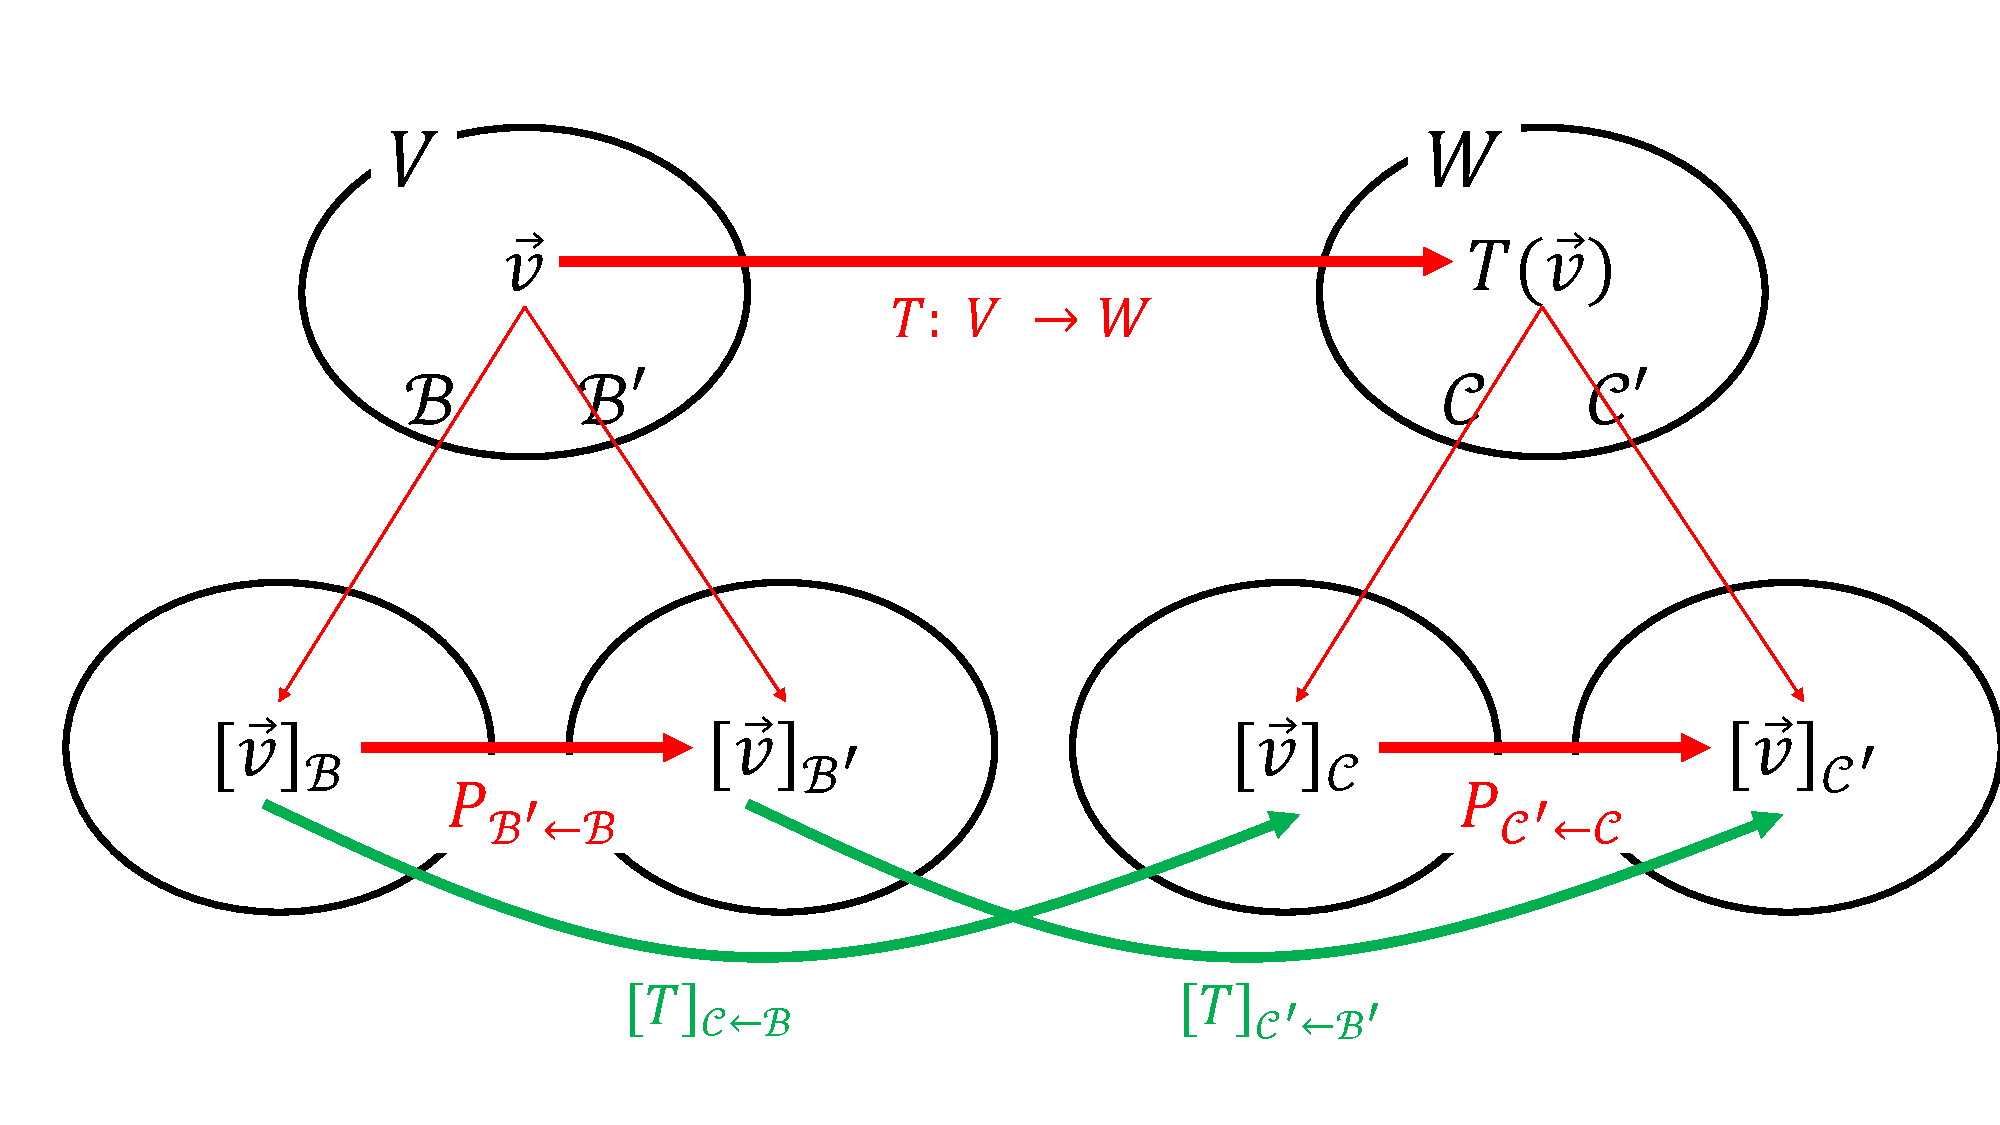
\includegraphics[scale = 0.4]{Figure3.pdf}
	\end{center}
\end{figure} By Theorem 6.12(a) and Theorem 6.12(c), for any vector $\textbf{v} \in V$ and $\textbf{w} \in W$, \begin{align*}
	[\textbf{v}]_{\mathcal{B}} = P_{\mathcal{B} \leftarrow \mathcal{B}'}[\textbf{v}]_{\mathcal{B}'} = \inv{( P_{\mathcal{B}' \leftarrow \mathcal{B}} )}[\textbf{v}]_{\mathcal{B}'}  \mbox{ and } [\textbf{w}]_{\mathcal{C}'} = P_{\mathcal{C}' \leftarrow \mathcal{C}}[\textbf{w}]_\mathcal{C}
\end{align*}
By Theorem 6.26, for every vector $\textbf{v} \in V$, \begin{equation*}
	[T]_{ \mathcal{C} \leftarrow \mathcal{B} }[\textbf{v}]_\mathcal{B} = [T(\textbf{v})]_\mathcal{C} \mbox{ and } [T]_{ \mathcal{C}' \leftarrow \mathcal{B}' }[\textbf{v}]_{\mathcal{B}'} = [T(\textbf{v})]_{\mathcal{C}'}
\end{equation*}
Therefore, for every vector $\textbf{v} \in V$, \begin{align*}
	P_{ \mathcal{C}' \leftarrow \mathcal{C} }[T]_{ \mathcal{C} \leftarrow \mathcal{B} }\inv{(P_{ \mathcal{B}' \leftarrow \mathcal{B}}) }[\textbf{v}]_{\mathcal{B}'} = P_{ \mathcal{C}' \leftarrow \mathcal{C} }[T]_{ \mathcal{C} \leftarrow \mathcal{B} }[\textbf{v}]_\mathcal{B} = P_{ \mathcal{C}' \leftarrow \mathcal{C} }[T(\textbf{v})]_\mathcal{C} = [T(\textbf{v})]_{\mathcal{C}'}
\end{align*}
Since $[T]_{ \mathcal{C}' \leftarrow \mathcal{B}' }$ is the unique matrix satisfying such property (Exercise 6.6 39), this implies that $[T]_{ \mathcal{C}' \leftarrow \mathcal{B}' } = P_{ \mathcal{C}' \leftarrow \mathcal{C} }[T]_{ \mathcal{C} \leftarrow \mathcal{B} }\inv{(P_{ \mathcal{B}' \leftarrow \mathcal{B}}) }$. \\

\textbf{(6.6 45)} \\
Let $\mathcal{B} = \{\textbf{v}_1, \cdots, \textbf{v}_n\}$ be a basis for $V$, and $\mathcal{C} = \{\textbf{w}_1, \cdots, \textbf{w}_m\}$ be a basis for $W$. Let $\Phi: \mathscr{L}(V, W) \rightarrow M_{mn}$ be a transformation defined by \begin{equation*}
	\Phi(T) = [T]_{ \mathcal{C} \leftarrow \mathcal{B} }
\end{equation*} for any linear transformation $T: V \rightarrow W$. \\

(i) For any $S, T \in \mathscr{L}(V, W)$ and any scalar $c$, \begin{align*}
	\Phi(S + T) &= [S + T]_{ \mathcal{C} \leftarrow \mathcal{B} } \\
	&= \begin{bmatrix}
		\left[(S + T)(\textbf{v}_1)\right]_\mathcal{C} & \cdots & \left[(S + T)(\textbf{v}_n)\right]_\mathcal{C}
	\end{bmatrix} \\
	&= \begin{bmatrix}
	\left[S(\textbf{v}_1) + T(\textbf{v}_1)\right]_\mathcal{C} & \cdots & \left[S(\textbf{v}_n) + T(\textbf{v}_n)\right]_\mathcal{C}
	\end{bmatrix} \\
	&= \begin{bmatrix}
	\left[S(\textbf{v}_1)\right]_\mathcal{C} & \cdots & \left[S(\textbf{v}_n)\right]_\mathcal{C}
	\end{bmatrix} + \begin{bmatrix}
	\left[T(\textbf{v}_1)\right]_\mathcal{C} & \cdots & \left[T(\textbf{v}_n)\right]_\mathcal{C}
	\end{bmatrix} \\
	&= [S]_{ \mathcal{C} \leftarrow \mathcal{B} } +  [T]_{ \mathcal{C} \leftarrow \mathcal{B} } = \Phi(S) + \Phi(T) \\
	\Phi(cT) &= [cT]_{ \mathcal{C} \leftarrow \mathcal{B} } \\
	&= \begin{bmatrix}
	\left[(cT)(\textbf{v}_1)\right]_\mathcal{C} & \cdots & \left[(cT)(\textbf{v}_n)\right]_\mathcal{C}
	\end{bmatrix} \\
	&= \begin{bmatrix}
	\left[cT(\textbf{v}_1)\right]_\mathcal{C} & \cdots & \left[cT(\textbf{v}_n)\right]_\mathcal{C}
	\end{bmatrix} \\
	&= c\begin{bmatrix}
	\left[T(\textbf{v}_1)\right]_\mathcal{C} & \cdots & \left[T(\textbf{v}_n)\right]_\mathcal{C}
	\end{bmatrix} = c[T]_{ \mathcal{C} \leftarrow \mathcal{B} } = c\Phi(T)
\end{align*} thus $\Phi$ is a linear transformation. \\

(ii) Let $T_1, T_2 \in \mathscr{L}(V, W)$ such that $\Phi(T_1) = \Phi(T_2)$, then $[T_1]_{ \mathcal{C} \leftarrow \mathcal{B} } = [T_2]_{ \mathcal{C} \leftarrow \mathcal{B} }$. Then for each $i = 1, 2, \cdots, n$, $[T_1(\textbf{v}_i)]_\mathcal{C}$ and $[T_2(\textbf{v}_i)]_\mathcal{C}$ are the same, so $T_1(\textbf{v}_i) = T_2(\textbf{v}_i)$. Let $\textbf{v} \in V$, then there exist scalars $c_1, \cdots, c_n$ such that $\textbf{v} = c_1\textbf{v}_1 + \cdots + c_n\textbf{v}_n$. Then \begin{align*}
	T_1(\textbf{v}) &= T_1(c_1\textbf{v}_1 + \cdots + c_n\textbf{v}_n) \\
	&= c_1T_1(\textbf{v}_1) + \cdots + c_nT_1(\textbf{v}_n) = c_1T_2(\textbf{v}_1) + \cdots + c_nT_2(\textbf{v}_n) \\
	&= T_2(c_1\textbf{v}_1 + \cdots + c_n\textbf{v}_n) = T_2(\textbf{v})
\end{align*} Therefore, $T_1 = T_2$, hence $\Phi$ is one-to-one. \\

(iii) Let $A$ be a $m \times n$ matrix. Let $T: V \rightarrow W$ be a transformation, which is defined by mapping \begin{equation*}
	T(\textbf{v}_i) = A_{1i}\textbf{w}_1 + \cdots + A_{mi}\textbf{w}_m
\end{equation*} for each $i = 1, 2, \cdots, n$, and for any vector $\textbf{v} \in V$, there exist scalars $c_1, \cdots, c_n$ such that $\textbf{v} = c_1\textbf{v}_1 + \cdots + c_n\textbf{v}_n$, then $T(\textbf{v})$ is defined as \begin{equation*}
	T(\textbf{v}) = c_1T(\textbf{v}_1) _+ \cdots + c_nT(\textbf{v}_n)
\end{equation*}
It is trivial from the definition that $T$ is a linear transformation. Also, the definition of $T$ also gives that $[T]_{ \mathcal{C} \leftarrow \mathcal{B} } = A$,  so $\Phi(T) = A$. Therefore, $\Phi$ is onto. \\

By (i), (ii), and (iii), $\Phi$ is an isomorphism, thus $\mathscr{L}(V, W) \cong M_{mn}$. \\

\textbf{(6.6 46)}
Let $n = \dim V$, then $V^\star = \mathscr{L}(V, W) \cong M_{n1}$ by Exercise 6.6 45. Therefore, $\dim V^\star = \dim M_{n1} = n = \dim V$, hence $V^\star \cong V$.
\fi